\documentclass[11pt,twoside,a4paper]{report}

\usepackage{fullpage}
\usepackage{amssymb}
\usepackage{pifont}
\usepackage{hyperref}
\usepackage{forest}
\usepackage{listings}
\usepackage{color}
\usepackage[round]{natbib}

\newcommand{\cmark}{\ding{51}}
\newcommand{\xmark}{\ding{55}}

\hypersetup{
    colorlinks=true, %set true if you want colored links
    linktoc=all,     %set to all if you want both sections and subsections linked
    linkcolor=blue,  %choose some color if you want links to stand out
}
\hypersetup{linktocpage} %in order to make only the numbers in the table of contents clickable

\forestset{
forestyle/.style={
	for tree={
		edge={<-,>=latex},
		l sep=1cm,
		circle,
		minimum size=12pt,
		anchor=west,
		where={iseven(level)}
			{edge={green!80},
			draw=green!80,
			fill=green!20
		}
			{edge={red!80},
			draw=red!80,
			fill=red!20
		},
		if={level>1}
		{s sep=1.3cm}
		{s sep=2cm}
	}
},
every node/.style={anchor=west,right,font=\sffamily,xshift=7pt,yshift=1pt}
}

\definecolor{dkgreen}{rgb}{0,0.6,0}
\definecolor{gray}{rgb}{0.5,0.5,0.5}
\definecolor{mauve}{rgb}{0.58,0,0.82}

\lstset{frame=tb,
  language=Prolog,
  aboveskip=3mm,
  belowskip=3mm,
  showstringspaces=false,
  columns=flexible,
  basicstyle={\small\ttfamily},
  numbers=left,
  numberstyle=\tiny\color{gray},
  keywordstyle=\color{blue},
  commentstyle=\color{dkgreen},
  stringstyle=\color{mauve},
  identifierstyle=\color{blue},
  breaklines=true,
  breakatwhitespace=true
  tabsize=3,
  captionpos=b
}

\author{Giorgos Flourentzos}
\title{Argumentation Logic Visualizer}
\begin{document}
\maketitle
\tableofcontents

\chapter{Introduction}

Formal logic is a standard method of giving validity to arguments. However, formal logic trivializes in the presence of inconsistencies, thus becoming inflexible when reasoning about inconsistent theories. Additionally, the Reductio ad Absurdum rule is used freely; under this rule the derived inconsistency can be reached without necessarily using the hypothesis assumed at the beginning of the rule's application. In argumentation, this translates to reaching a conclusion with an argument that has nothing to do with the topic of the conversation.

Argumentation Logic is a new argumentation framework proposed by Professor Antonis Kakas (University of Cyprus, Cyprus), Professor Paolo Mancarella (Universit\'a di Pisa, Italy) and Dr Francesca Toni (Imperial College London, United Kingdom). It is a framework based on propositional logic that allows reasoning closer to the way humans do. Argumentation Logic does not trivialize in the presence of inconsistencies.

Argumentation Logic is largely based on the already established natural deduction system. The major difference however lies in the fact that it restricts the use of the Reductio ad Absurdum (known as "not introduction") rule in a way that the assumed hypothesis must be critical to the application of that rule. Argumentation Logic can be seen from an argumentative point of view, as a debate between a proponent who puts forth arguments and defends them against an opponent, who in turn tried to attack those arguments. The arguments are sets of propositional sentences. The argument of the proponent is successful and a conclusion is therefore drawn if it can be successfully defended against the attacks made by the opponent. Argumentation Logic is a recent addition to the field of logic and remains partly unexplored.

The idea is to implement a simple and flexible GUI that will allow for the construction of valid propositional Argumentation Logic natural deduction proofs. In addition, the implemented software will be able to visualize the proofs as exchanges of arguments between proponent and opponent. This is an attempt to enable further research and study of Argumentation Logic as an established method for reasoning about potentially inconsistent environments in a human-like way, with potential applications in artificial intelligence.
The project is split into seven steps which build on top of each other.

\section{Step 1: Basic Natural Deduction Proof System}
The first step requires a natural deduction proof system that can find the steps required to reach a goal, given the theory and the goal that must be met. The aim of this step is to provide the basis on which to build the Argumentation Logic framework.

\section{Step 2: Improving the Proof System}
The second step requires the natural deduction proof system to be able to produce proofs with natural deduction rules applied with variable and configurable priorities and have the ability to look for proofs of a particular maximum length. This step might not be required depending on the implementation of the proof system in the previous step. Therefore the aim of this stage is to only facilitate the implementation of the proof system and has no bearing on the exploration of Argumentation logic.

\section{Step 3: Genuine Absurdity Property}
The third step involves the processing of produced natural deduction proofs in order to check the presence of the Genuine Absurdity Property. This property is closely tied to the identification of natural deduction proofs that are compatible with (that is, supported by) Argumentation Logic. Compatible proofs can be visualized as arguments between two debaters as in the following step.

\section{Step 4: Argumentation Logic Visualization}
The fourth step requires the construction of a GUI that allows the visualization of Argumentation Logic proofs as sets of arguments. The GUI can feature several extensions such as step-by-step building of an Argumentation Logic proof, saving and loading generated proofs, conversion between natural deduction and argumentation and so on.

\section{Step 5: Converting Natural Deduction Proofs to Argumentation Logic Proofs}
The fifth step revolves around the conversion of natural deduction proofs that are unsupported by Argumentation Logic (proofs that do not follow the Genuine Absurdity Property) to compatible ones. It can be shown in the technical report on Argumentation Logic that any proof not following the Genuine Absurdity Property can be converted to one that does. The aim of this step is to allow the possibility of virtually any natural deduction proof to be visualized from an argumentative view.

\section{Step 6: Re-Introduction of Disjunction and Implication Connectives}
The sixth step involves the introduction of the disjunction and implication connectives. It is shown in the technical report on Argumentation Logic that for consistent theories using only conjunction and negation, Propositional Logic is equivalent to Argumentation Logic. The use of disjunction and implication remain partly subject for future work. The aim of this step is to explore further this area.

\section{Step 7: Paraconsistency}
The seventh and final step ventures into how Argumentation Logic can allow for reasoning within an inconsistent environment. The aim of this step is to probe the notion of para-consistency of Argumentation Logic.

In conclusion, this project explores the premise of Argumentation Logic, a recent framework based on natural deduction of propositional logic that allows proofs to be visualized as an exchange of arguments. To aid the understanding of Argumentation Logic, a software will be created that enables the construction and visualization of proofs that adhere to this logic. At the time of writing, there is no published work in this area, and the nature of this project is investigative.

\chapter{Background}

\section{Argumentation Theory}
\label{sec:argtheory}
Recommended Reading: \citep*{argumentationinai}

\subsection{What is Argumentation Theory}
Exactly what defines an argument varies between different sources in argumentation theory. Douglas Walton defines an argument as being made of three parts: a conclusion, the premises based on which the conclusion is derived and an inference, which links the premises to the conclusion. Arguments are sets of propositions of some format and they tend to attack or defend other arguments in a conversation. They can be used in order to choose a course of action, decide for or against a decision, or find common ground between two (or more) parties. There are several packages that draw arguments as chains of attacks and defenses which will be discussed briefly in \autoref{sec:vizargtools}.

Argumentation differs from the traditional approaches of inference based on deductive logic. The difference lies in that traditional approaches (such as propositional calculus) prove that the conclusion sought after does indeed derive from the given premises. The conclusion and theory are both known in advance, and a single inference is made to link the two. This is called a monological approach. On the contrary, argumentation involves a process that looks more like a dialogue (hence it is a dialogical approach) which tries to look at the pros and cons of an argument. The process involves analyzing the arguments set forth for and against the initial argument, and finding strengths and weaknesses. The final outcome is then based on the strongest argument.

\subsection{Attacking Arguments}
There are different ways to attack an argument. Asking a critical question that raises doubt about a previous argument leads to that argument being refuted unless the other party can respond with a satisfactory answer. Questioning an argument's premises or inference is another way of attack. Putting forward a counter-argument (an argument that reaches the opposite conclusion of the first argument) or arguing that the premises are irrelevant to the conclusion (this problem, introduced by the Reductio ad Absurdum rule concerns Argumentation Logic) are also valid attacks. Different views exist about what constitutes an attack and what not; for example, Krabbe suggests his own seven ways to react to an argument \citep*{reasonreclaimed}.

\subsection{Types of Arguments}
Generally, arguments belong to three different categories, based on how the inference that links the conclusion to the evidence was made: deductive, inductive and defeasible. Defeasible arguments are different from inductive in that they cannot be anticipated statistically. For example, "Adults can drive. I am an adult. Therefore, I can drive." is an example of deductive reasoning, but in a defeasible environment it could be the case that I still cannot drive because of a broken leg. Argumentation Logic, as it is based on natural deduction, involves arguments of the deductive kind.

\subsection{Argumentation Example}
An example of an argument between two parties is given below:

\begin{enumerate}
\item
Student: Higher grades mean higher employability. Decreasing the volume of the curriculum will increase student performance and allow them to get higher marks. Therefore, we should decrease the volume of taught material.
\item
Director of Studies: How do you know that decreasing the volume of the material taught will improve students' marks?
\item
Student: Students will have more time to digest the curriculum and revise for the exams. In that way, they will achieve higher marks in the exams and overall grades.
\item
Director of Studies: Weakening the curriculum will make your degree less desirable at the same time, thus reducing your employability.
\item
Student: How do you know that our degree will become less important?
\item
Director of Studies: Reports we have gathered from the industry indicate that students from this university are of high demand because of their vast knowledge of material not covered in most other universities.
\end{enumerate}

The student sets the premise by stating that higher grades imply higher employability and smaller curriculum implies higher grades. His conclusion is that the taught material should be decreased. The director of studies attacks the student's argument by challenging the second premise. The student tries to defend himself by providing a concrete argument as to how a smaller curriculum can lead to better grades. The director of studies cannot attack that argument, and thus poses a different (yet relevant) argument: reducing the material offered will make the degree less attractive.  The student then attacks this argument by questioning it (the same way the director of studies questioned the student's initial argument). In the end, the director supplies facts that support his argument, leading to a counter-example that suggests that cutting down the curriculum will actually result in lower employability. The debate ends, as the student can no longer support his argument.

\subsection{Relevance}
\label{subsec:relevance}
As briefly mentioned before, irrelevance is one type of fallacy concerning argumentation theory. Under this fallacy, a debater can put forth an argument with premises that are of no relevance to the conversation at hand, perhaps stray away into a different matter and reach a conclusion that otherwise could not be met. Alternatively, this issue could cause the conversation to lead to nowhere. This will be discussed further when explaining how Argumentation Logic restricts the use of the Reductio ad Absurdum rule in order to establish a form of relevance (as seen in \autoref{subsec:gap}).

\subsection{Abstract Argumentation Framework}
\label{subsec:abrstrargframework}
An argumentation framework is a framework that is established in order to allow for formal study of argumentation theory. Perhaps the most basic argumentation framework is the widely known abstract argumentation framework \citep*{dung95}. This is a very simple framework that is defined by a set containing the arguments set forth by a party and the attack relation, a binary relation that defines which argument in the set attacks which.

In formal notation, an abstract argumentation framework is usually given by the tuple
\[\langle Args, Att\rangle\]
where:
\begin{itemize}
\item
Args is the set of all possible arguments that are relevant to the subject modeled by the argumentation framework
\item
Att is the binary relation $Args\times Args$ where a $(a, b)\in Att$ means that argument $a$ attacks argument $b$.
\end{itemize}

For example consider the small abstract argumentation framework that models the possibility of going hiking if it is raining. Assume for this example that going hiking is not possible if it is raining, unless a raincoat is at hand. Additionally, not going hiking on a beautiful sunny day is out of the question, unless of course it happens to be very muddy (from the rain the night before).

Our arguments can be $c$ for having a raincoat, $r$ to indicate that it is raining, $h$ for deciding to go on a hike, $h'$ for deciding against hiking, $s$ for being sunny and finally $m$ for being muddy. Thus $Args = \{c, r, h, h', s, m\}$.

In this framework, argument $r$ attacks argument $h$ (rain does not allow hiking), and argument $c$ attacks argument $r$ (having a raincoat guards against the rain). Also, $s$ attacks $h'$ (as it would be a shame to not go hiking on a sunny day) and $m$ attacks $s$ (since a lot of mud will incur a lot of hand-washing later on). Arguably, $h$ attacks $h'$ and vice-versa, as the two arguments are mutually exclusive. Thus $Att = \{(r, h), (c, r), (s, h'), (m, s), (h, h'), (h', h)\}$.

The abstract argumentation framework resulting from this example will then be of the form $\langle Args, Att\rangle$.

There are very many extensions to Dung's abstract argumentation framework for different reasons, such as aiming to cover limitations of this framework or tailoring it to better fit particular domains. Examples of extensions of this framework are the abstract bipolar argumentation framework \citep*{bipolarAA}, assumption-based argumentation \citep*{aba}, logic-based argumentation frameworks \citep*{logicAA} and value-based argumentation frameworks \citep*{valueAA}.

It will be seen later on in \autoref{subsec:alfdef} that Argumentation Logic establishes its own framework by building directly on top of an abstract argumentation framework.

\subsection{Visualization of Abstract Argumentation Framework}
\label{subsec:aafviz}
An abstract argumentation framework can be seen from a graphical point of view. The arguments $Args$ form nodes in a graph, and the attack relation $Att$ forms the edges. The above example, with $\langle Args, Att\rangle$ (where $Args = \{c, r, h, h', s, m\}$ and $Att = \{(r, h), (c, r), (s, h'), (m, s), (h, h'), (h', h)\}$), can be visualized in \autoref{fig:aafviz}.

\begin{figure}
\centerline{\begin{forest}
forestyle
[,tikz={\node[pos=0,font=\sffamily,anchor=west,xshift=12pt,yshift=1pt]{h};}
	[,edge label={node[font=\sffamily,anchor=west,xshift=8pt,yshift=1pt]{\color{black}r}}
		[,edge label={node[font=\sffamily,anchor=west,xshift=12pt,yshift=1pt]{\color{black}c}}]
	]
    [,edge={<->}, edge label={node[font=\sffamily,anchor=west,xshift=8pt,yshift=1pt]{\color{black}h'}}
    	[,edge label={node[font=\sffamily,anchor=west,xshift=12pt,yshift=1pt]{\color{black}s}}
    		[,edge label={node[font=\sffamily,anchor=west,xshift=12pt,yshift=1pt]{\color{black}m}}]
    	]
	]
]
\end{forest}}
\caption{Visualization of abstract argumentation example in \autoref{subsec:abrstrargframework}\label{fig:aafviz}}
\end{figure}

\section{Natural Deduction}
\label{sec:nd}
Recommended Reading: \citep*[pp. 17-225]{languageproofandlogic}

\subsection{Rules for Propositional Logic}
\label{subsec:logicrules}
The rules for propositional logic used throughout this paper are as follows:

\begin{tabular}{|c|c|c|c|c|c|}
\hline
$\wedge I:\frac{\phi, \psi}{\phi\wedge\psi}$ &
$\wedge E:\frac{\phi\wedge\psi}{\psi}$ &
$\wedge E:\frac{\phi\wedge\psi}{\phi}$ &
$\vee I:\frac{\psi}{\phi\wedge\psi}$ & 
$\vee I:\frac{\phi}{\phi\wedge\psi}$ &
$\vee E:\frac{\phi\vee\psi, [\phi...\chi], [\psi...\chi]}{\chi}$ \\
\hline
$\rightarrow I:\frac{[\phi...\psi]}{\phi\rightarrow\psi}$ & 
$\rightarrow E:\frac{\phi, \phi\rightarrow\psi}{\psi}$ &
$\neg I:\frac{[\phi...\bot]}{\neg\phi}$ &
$\neg E:\frac{\neg\neg\phi}{\phi}$ &
$\bot I:\frac{\phi, \neg\phi}{\bot}$ &
$\bot E:\frac{\bot}{\phi}$ \\
\hline
\end{tabular}

Note: the notation $[\phi...\psi]$ means a derivation of $\psi$ with hypothesis $\phi$.

\subsection{Example of Natural Deduction Proof}
An example of a natural deduction proof can be shown below. The format of natural deduction proofs will follow the format of this example:

Assume theory $T = \{\alpha\rightarrow\beta\rightarrow\neg\gamma, \neg\gamma\wedge\beta\}$ and prove $\neg\alpha$.

\[\vbox{\offinterlineskip\halign{
&\tabskip=1.5em#\strut&$#$\hfil\tabskip=1em&\hfil$#$\tabskip=0em\cr
%
1&\alpha\rightarrow\beta\rightarrow\gamma&\mbox{given}\cr
2&\neg\gamma\wedge\beta&\mbox{given}\cr
%
\multispan3\vbox{\halign{
\vrule#&&\hskip.1em\tabskip=1em#\strut&$#$\hfil\tabskip=1em&\hfil$#$\hskip0.1em\tabskip=0em&\vrule#\cr
\noalign{\hrule}
%
&3&\alpha&\mbox{hypothesis}&\cr
&4&\beta\rightarrow\neg\gamma&\rightarrow E(1,3)&\cr
&5&\beta&\wedge E(2)&\cr
&6&\gamma&\rightarrow E(1,5)&\cr
&7&\neg\gamma&\wedge E(2)&\cr
&8&\bot&\bot I(6,7)&\cr
%
\noalign{\hrule}}}\,\cr
%
9&\neg\alpha&\neg I(3,8)\cr
}}\]

A box is used to contain the hypotheses, derivations inside which cannot be used outside. Each derivation is numbered on the left, and reasons (i.e. rules used) for each derivation are given on the right, following the rules defined in the previous section. Theory is indicated as "given", and assumptions (hypotheses) are indicated as "hypothesis" at the beginning of a sub-derivation (inner box). Sub-derivations can also be indicated as $[\phi ... \bot]$ in the text, where $\phi$ is the hypothesis.

\subsection{Automated Theorem Proving and Proof Search}
\label{subsec:nnd}
Despite what the name implies, proof theory in general does not work with natural deduction calculi as the expressiveness of natural deduction comes at a price in terms of its unrestricted search space \citep*[pp. 140-141]{siegfried}. Hilbert systems and natural deduction are said to be inappropriate for automated theorem proving since they both exhibit the modus ponens rule \citep*[p. 95]{autobots}. Natural deduction calculi that are indeed used in theorem proving or proof search have special properties and restrictions in their search space in order to provide a good strategic method of achieving their goals \citep*[pp. 140-141]{siegfried}.

\subsection{Example of a Proof Search Implementation}
\label{subsec:carnage}
The \href{http://www.cs.cmu.edu/~cogito/cptproject.html}{Carnegie Mellon Proof Tutor}\footnote{http://www.cs.cmu.edu/~cogito/cptproject.html} is an example of an automated proof search program that can formulate proofs in natural deduction by employing a wide range of natural deduction proofs. A summary of its ruleset (with a slight adjustment to the notation) is given below:

Using the notation in Sieg and Scheine's article \citep{siegfried}, $\alpha;\beta?G$ is a triplet describing the following:
\begin{itemize}
\item
available assumptions as the set of formulas $\alpha$
\item
set of formulas obtained by using the $\wedge E$ and $\rightarrow E$ rules on the available assumptions $\beta$
\item
current goal $G$
\end{itemize}

The following conventions are used in the article: the concatenation of sequences $\alpha$ and $\beta$ is indicated by their juxtaposition; if $\phi$ is a formula and $\alpha$ is a sequence, then the extension of $\alpha$ by $\phi$ is given by $\alpha,\phi$; lastly, a formula $\phi$ that is a member of the sequence $\alpha$ can be denoted by $\phi \in \alpha$.

The rules used by this proof search program are split into three categories, namely the elimination rules ($\downarrow$-rules), the introduction rules ($\uparrow$-rules) and the negation rules. 

The elimination rules are listed here:
\begin{itemize}
\item
$r\downarrow\wedge_i:\alpha,\beta?G, \phi_1\wedge\phi_2 \in \alpha\beta, \phi_i \notin \alpha\beta \Rightarrow \alpha;\beta,\phi_i?G, i = 1\, or\, 2$

(if there is a conjunction in the set $\alpha\beta$, add its components if not already present)
\item
$r\downarrow\vee:\alpha,\beta?G, \phi_1\vee\phi_2 \in \alpha\beta, \phi_1 \notin \alpha\beta, \phi_2 \notin \alpha\beta \Rightarrow \alpha,\phi_1?G\, AND\, \alpha,\phi_2?G$

(if there is a disjunction in the set $\alpha\beta$, and neither of the components have been proven, do a case by case analysis on the goal)
\item
$r\downarrow\rightarrow\alpha,\beta?G, \phi_1\rightarrow\phi_2 \in \alpha\beta, \phi_1 \in \alpha\beta, \phi_2 \notin \alpha\beta \Rightarrow \alpha;\beta,\phi_2?G$

(if there is an implication in the set $\alpha\beta$ and the first component has been proven, add the second component to the set $\beta$ if not already present)
\end{itemize}

Note that the restricted versions of the elimination rules are to be used in the proof search implementation (hence the "r" in front of the rules' names) so that redundancy is avoided. The restricted rules only add elements if they are absent from the set $\alpha\beta$. Otherwise, the system could hang by adding infinite copies of the same formulas by repeatedly applying the unrestricted rules. The restrictions in the above rules are the $\phi_i \notin \alpha\beta$ conditions not present in the unrestricted versions.

Consider for example the query $\alpha,\beta?G$ where $\alpha = \{\gamma\wedge\delta\}, \beta = \{\gamma\}$ and $G = \delta$. If the restriction $\gamma \notin \{\gamma\wedge\delta\}$ was not present, then the first elimination rule would be applicable all the time, and the program could keep adding $\gamma$ to the set $\beta$ forever, making no real progress.

The introduction rules are listed here:
\begin{itemize}
\item
$\uparrow\wedge: \alpha;\beta?\phi_1\wedge\phi_2 \Rightarrow \alpha;\beta?\phi_1\, AND\, \alpha;\beta?\phi_2$

(if the goal is a conjunction, prove its constituent parts)
\item
$\uparrow\vee: \alpha;\beta?\phi_1\vee\phi_2 \Rightarrow \alpha;\beta?\phi_1\, OR\, \alpha;\beta?\phi_2$

(if the goal is a disjunction, prove either of its constituent parts)
\item
$\uparrow\rightarrow: \alpha;\beta?\phi_1\rightarrow\phi_2 \Rightarrow \alpha,\phi_1;?\phi2$

(if the goal is an implication, assume the first part and prove the second)
\end{itemize}

The negation rules are listed here:
\begin{itemize}
\item
$\bot_c: \alpha;\beta?\phi, \phi\neq\bot \Rightarrow \alpha,\neg\phi;?\bot$

(proof by contradiction: if the goal is a positive formula other than contradiction, prove that its negation leads to a contradiction)
\item
$\bot_i: \alpha;\beta?\neg\phi \Rightarrow \alpha,\phi;?\bot$

(if the goal is a negated formula, prove that the positive subformula leads to a contradiction)
\item
$\bot_F: \alpha;\beta?\bot, \phi\in F \Rightarrow \alpha;\beta?\phi\, AND\, \alpha;\beta?\neg\phi$

(if the goal is a contradiction, prove it by taking any subformula in the set $\alpha\beta$ and prove both that subformula and its negation)
\end{itemize}

The last rule mentions $F$; this is the finite class of formulas that consist of all subformulas of elements in the subsequence $\alpha\beta$. The theorem prover built for this project (\autoref{chap:prover}) will base some of its rules on the Carnegie Mellon Proof Tutor.

\section{Argumentation Logic}
Recommended Reading: \citep*{alpaper}

\subsection{Introduction}
This section gives a brief introduction of the concepts behind Argumentation Logic, as found in the technical report. Section Exploring Argumentation Logic shows how these concepts are used to build the visualization tool.

Argumentation Logic builds a bridge between argumentation theory and propositional logic. This duality is formed by combining notions from both argumentation theory and natural deduction. For consistent theories, Argumentation Logic is equivalent to propositional logic, but it also extends into a para-consistent logic for inconsistent theories. From the argumentation point of view, Argumentation Logic can be seen as arguments that are sets of propositional formulas that attack and defend against other arguments. From the propositional logic point of view, Argumentation Logic can be seen as a natural deduction system that restricts the use of the Reductio ad Absurdum rule in order to allow for relevant arguments to be used only. The rest of this section is devoted to explaining the concepts behind this new logic.

\subsection{Argumentation Logic Framework}
In order to establish the Argumentation Logic framework, the notions of "direct derivation" and "direct consistency" must first be defined:

\subsubsection{Direct Derivation}
A direct derivation for a sentence from a theory is a natural deduction derivation of that sentence from the given theory that does not contain any application of the Reductio ad Absurdum rule. If such a derivation exists, then we say that this sentence is directly derived (derived modulo RA) from the theory. For a sentence $\phi$ directly derived from theory $T$, we denote $T\vdash_{MRA} \phi$.
For example, assume theory $T = \{\alpha\rightarrow\beta, \beta\rightarrow\delta\}$, and derive $\alpha\rightarrow\delta$:

\[\vbox{\offinterlineskip\halign{
&\tabskip=1.5em#\strut&$#$\hfil\tabskip=1em&\hfil$#$\tabskip=0em\cr
%
1&\alpha\rightarrow\beta&\mbox{given}\cr
2&\beta\rightarrow\delta&\mbox{given}\cr
%
\multispan3\vbox{\halign{
\vrule#&&\hskip.1em\tabskip=1em#\strut&$#$\hfil\tabskip=1em&\hfil$#$\hskip0.1em\tabskip=0em&\vrule#\cr
\noalign{\hrule}
%
&3&\alpha&\mbox{hypothesis}&\cr
&4&\beta&\rightarrow E(1,3)&\cr
&5&\delta&\rightarrow E(2,4)&\cr
%
\noalign{\hrule}}}\,\cr
%
9&\alpha\rightarrow\delta&\neg I(3,5)\cr
}}\]

This is a direct derivation as the Reductio ad Absurdum rule was not used.

As another example, assume theory $T = \{\alpha\rightarrow\bot\}$ and derive $\neg\alpha$:

\[\vbox{\offinterlineskip\halign{
&\tabskip=1.5em#\strut&$#$\hfil\tabskip=1em&\hfil$#$\tabskip=0em\cr
%
1&\alpha\rightarrow\bot&\mbox{given}\cr
%
\multispan3\vbox{\halign{
\vrule#&&\hskip.1em\tabskip=1em#\strut&$#$\hfil\tabskip=1em&\hfil$#$\hskip0.1em\tabskip=0em&\vrule#\cr
\noalign{\hrule}
%
&3&\alpha&\mbox{hypothesis}&\cr
&4&\bot&\rightarrow E(1,2)&\cr
%
\noalign{\hrule}}}\,\cr
%
9&\neg\alpha&\neg I(2,3)\cr
}}\]

This is not a direct derivation as the Reductio ad Absurdum rule had to be used.

\subsubsection{Classical and Direct Consistency/Inconsistency}
The word "classical" is used to denote the original natural deduction entailment. The word "direct" uses the notion above. A theory is classically inconsistent if a contradiction can be derived from it in the "classical" sense. A theory is directly inconsistent if a contradiction can be derived through a direct derivation. A theory is classically or directly consistent if it is not classically or directly inconsistent, respectively.

In notation, a theory $T$ is
\begin{itemize}
\item
classically inconsistent if $T\vdash\bot$
\item
directly inconsistent if $T\vdash_{MRA}\bot$
\item
classically consistent if $T\nvdash\bot$
\item
directly consistent if $T\nvdash_{MRA}\bot$
\end{itemize}

In a sense, direct derivation capabilities form a subset of those of the classical derivation. Hence, if a theory is classically consistent then it is directly consistent too. A directly consistent theory can be classically inconsistent however, since classical derivation has one more rule for proving contradiction (namely, the Reductio ad Absurdum rule) that direct derivation does not have.

As an example, consider theory $T = \{\alpha\rightarrow\beta, \neg\alpha\rightarrow\gamma, \neg\beta\wedge\neg\gamma\}$ and prove contradiction:

\[\vbox{\offinterlineskip\halign{
&\tabskip=1.5em#\strut&$#$\hfil\tabskip=1em&\hfil$#$\tabskip=0em\cr
%
1&\alpha\rightarrow\beta&\mbox{given}\cr
2&\neg\alpha\rightarrow\gamma&\mbox{given}\cr
3&\neg\beta\wedge\neg\gamma&\mbox{given}\cr
%
\multispan3\vbox{\halign{
\vrule#&&\hskip.1em\tabskip=1em#\strut&$#$\hfil\tabskip=1em&\hfil$#$\hskip0.1em\tabskip=0em&\vrule#\cr
\noalign{\hrule}
%
&4&\alpha&\mbox{hypothesis}&\cr
&5&\beta&\rightarrow E(1,4)&\cr
&6&\neg\beta&\wedge E(3)&\cr
&7&\bot&\bot I(5,6)&\cr
%
\noalign{\hrule}}}\,\cr
%
8&\neg\alpha&\neg I(4,7)\cr
9&\gamma&\rightarrow E(2,8)\cr
10&\neg\gamma&\wedge E(3)\cr
11&\bot&\bot I(9,10)\cr
}}\]

This proof requires the use of the Reductio ad Absurdum rule, without which a contradiction cannot be derived. Thus, this theory is classically inconsistent, but directly consistent.

\subsubsection{Argumentation Logic Framework Definition}
\label{subsec:alfdef}
The Argumentation Logic framework relies on Dung's abstract argumentation framework as defined in \autoref{subsec:abrstrargframework}. It involves a set of arguments (where each argument is a set of propositional sentences) and the attack relation between the arguments. Thus for a given theory $T$, the Argumentation Logic framework becomes
\[\langle Args^T, Att^T\rangle\]
where:
\begin{itemize}
\item
$Args^T = \{T\cup\Sigma\}$ where $\Sigma$ is a set of propositional formulas. Hence all arguments include the starting theory $T$ and potentially more propositional formulas $\Sigma$
\item
$Att^T = \{(b,a) | a,b \in Args^T, a = T\cup\Delta, \Delta\neq\{\}, b = T\cup\Gamma, T\cup\Delta\cup\Gamma\vdash_{MRA}\bot\}$, that is, a set of pairs of arguments, the union of which provides ground for the direct derivation of a contradiction. In other words, $Att^T$ contains all pairs of arguments that don't agree with each other!
\end{itemize}

Since the theory is fixed for the argumentation framework, any argument $a = T\cup\Sigma$  will be referred to only by $\Sigma$. The argument $T\cup\{\}$ will thus be referred to as the empty argument. Note that in the attack relation, the attacked argument cannot be empty and apart from this exception, all attacks are reflexive.
As an example, consider $T = \{\alpha\rightarrow\beta, \alpha\rightarrow\gamma\}$. Here, $\{a\}$ attacks (and is attacked by) $\{\neg\beta\}$ or $\{\neg\gamma\}$. For a directly inconsistent theory, all arguments are hostile to each other since a contradiction can be derived from any possible pair of arguments (the empty argument can still not be attacked).

\subsubsection{Defense Against an Attack}
\label{subsec:alfdef2}
Using the Argumentation Logic framework described above, and taking any argument $a = T\cup\Delta$, an argument $d$ can be described as a defense against $a$ if any of the following is true:
\begin{itemize}
\item
$d = T\cup\{\neg\phi\}$ or $d = T\cup\{\phi\}$ for some sentence $\phi\in\Delta$ or $\neg\phi\in\Delta$ respectively
\item
$d = T\cup\{\}$ and $a\vdash_{MRA}\bot$
\end{itemize}

What this means is that argument $d$ can take an opposing view on one of the sentences in argument $a$ (this can be interpreted as questioning one of the premises or the conclusion of an argument in argumentation theory) or if argument $a$ is self-contradicting, then saying nothing (empty argument) still counts as a defense against that argument.

\subsection{Acceptability Semantics}
This section defines what it means for an argument to be acceptable in Argumentation Logic, as discussed in the technical report.

\subsubsection{Acceptability of Arguments}
Given an argumentation framework $\langle Args^T, Att^T\rangle$ as discussed in the previous section fixed for a consistent theory $T$, with $a,b\in Args^T$, then $a$ is acceptable with respect to $b$, denoted by $ACC^T(a,b)$, if and only if either of the following conditions is met:
\begin{itemize}
\item
$a\subseteq b$
\item
for all $c\in Args^T$ such that $(c,a)\in Att^T$ both of the following are true:
\begin{itemize}
\item
$c\nsubseteq a\cup b$
\item
there is an argument $d\in Args^T$ which defends against $c$ and $ACC^T(d,a\cup b)$
\end{itemize}
\end{itemize}

Intuitively, an argument is acceptable with respect to one other one if it is a subset of it (they share the same ideas), or all of its attacking arguments are not based on the same ideas (are not subsets of the two arguments whose acceptability is under examination) and they can be successfully blocked by other acceptable arguments.

\subsubsection{Non-Acceptability of Arguments}
\label{subsec:nacc}
Similarly to the acceptability of arguments, for argumentation framework $\langle Args^T, Att^T\rangle$ fixed for a consistent theory $T$, with $a,b\in Args^T$, then $a$ is not acceptable with respect to $b$, denoted by $NACC^T(a,b)$, if and only if both of the following conditions are met:
\begin{itemize}
\item
$a\nsubseteq b$
\item
there is an argument $c\in Args^T$ such that $(c,a)\in Att^T$ and either of the following is true:
\begin{itemize}
\item
$c\subseteq a\cup b$
\item
for all arguments $d\in Args^T$ which defend against $c$ it is true that $NACC^T(d,a\cup b)$
\end{itemize}
\end{itemize}

Intuitively, an argument is unacceptable with respect to another if they are different and there is an attacking argument that comes from the same ideas as the arguments under examination and it cannot be defended against (by an acceptable argument). Note that non-acceptability is the exact opposite of acceptability, and so it holds that $NACC^T(a,b) = \neg ACC^T(a,b)$.

\subsubsection{Example of Non-Acceptability}
Consider theory $T = \{\alpha\wedge\beta\rightarrow\bot, \neg\beta\wedge\gamma\rightarrow\bot, \neg\gamma\wedge\delta\rightarrow\bot\}$. $NACC^T(\{a\},\{\})$ holds, because:
\begin{itemize}
\item
$\{a\}\nsubseteq\{\}$, $\{\beta\}$ attacks $\{\alpha\}$ and $\{\neg\beta\}$ is the only defense against $\{\beta\}$, and so it suffices to show that $NACC^T(\{\neg\beta\}, \{\alpha\})$
\item
$\{\neg\beta\}\nsubseteq\{\alpha\}$, $\{\gamma\}$ attacks $\{\neg\beta\}$ and $\{\neg\gamma\}$ is the only defense against $\{\gamma\}$, and so it suffices to show that $NACC^T(\{\neg\gamma\}, \{\alpha\, \neg\beta\})$
\item
$\{\neg\gamma\}\nsubseteq\{\alpha, \neg\beta\}$, $\{\delta\}$ attacks $\{\neg\gamma\}$ and there is unfortunately no defense against it, thus $NACC^T(\{\neg\gamma\}, \{\alpha,\neg\beta\})$, $NACC^T(\{\neg\beta\}, \{\alpha\})$ and in turn $NACC^T(\{\alpha\}, \{\})$ all hold
\end{itemize}

\subsection{Reductio ad Absurdum, Genuine Absurdity Property and Acceptability Semantics}
This section introduces the Genuine Absurdity Property, and relates it to the use of the Reductio ad Absurdum rule and the acceptability semantics.

\subsubsection{RAND Derivations}
\label{subsec:rand}
Reductio ad Absurdum derivations (RAND for short) are natural deduction derivations that are enclosed by a Reductio ad Absurdum rule application. 

Thus a RAND derivation of a propositional formula $\neg\phi$ is a natural deduction derivation of $\neg\phi$ which starts with a hypothesis $\phi$ and reaches a contradiction, allowing for the Reductio ad Absurdum rule to be applied in order to deduce $\neg\phi$.

A sub-derivation (of a certain derivation) is a RAND sub-derivation (of that derivation) if the sub-derivation itself is a RAND derivation. Hence a tree can be formed with the RAND derivation as the root, its RAND sub-derivations as its immediate children, the RAND sub-sub-derivations as the next node level, and so on.

Consider as an example, theory $T = \{\alpha\rightarrow\bot, \beta\rightarrow\bot, \neg\alpha\wedge\neg\beta\wedge\gamma\rightarrow\bot\}$ and prove $\neg\gamma$.

\[\vbox{\offinterlineskip\halign{
&\tabskip=1.5em#\strut&$#$\hfil\tabskip=1em&\hfil$#$\tabskip=0em\cr
%
1&\alpha\rightarrow\bot&\mbox{given}\cr
2&\beta\rightarrow\bot&\mbox{given}\cr
3&\neg\alpha\wedge\neg\beta\wedge\gamma\rightarrow\bot&\mbox{given}\cr
%
\multispan3\vbox{\halign{
\vrule#&&\hskip.1em\tabskip=1em#\strut&$#$\hfil\tabskip=1em&\hfil$#$\hskip0.1em\tabskip=0em&\vrule#\cr
\noalign{\hrule}
%
&4&\gamma&\mbox{hypothesis}&\cr
%
&\multispan3\,\vbox{\halign{
\vrule#&&\hskip.1em\tabskip=1em#\strut&$#$\hfil\tabskip=1em&\hfil$#$\hskip0.1em\tabskip=0em&\vrule#\cr
\noalign{\hrule}
%
&5&\alpha&\mbox{hypothesis}&\cr
&6&\bot&\rightarrow E(1,5)&\cr
%
\noalign{\hrule}}}\,&\cr
%
&7&\neg\alpha&\neg I(5,6)&\cr
%
&\multispan3\,\vbox{\halign{
\vrule#&&\hskip.1em\tabskip=1em#\strut&$#$\hfil\tabskip=1em&\hfil$#$\hskip0.1em\tabskip=0em&\vrule#\cr
\noalign{\hrule}
%
&8&\beta&\mbox{hypothesis}&\cr
&9&\bot&\rightarrow E(2,8)&\cr
%
\noalign{\hrule}}}\,&\cr
%
&10&\neg\beta&\neg I(8,9)&\cr
&11&\neg\alpha\wedge\neg\beta&\wedge I(7,10)&\cr
&12&\neg\alpha\wedge\neg\beta\wedge\gamma&\wedge I(4,11)&\cr
&13&\bot&\bot I(4,12)&\cr
%
\noalign{\hrule}}}\,\cr
%
14&\neg\gamma&\neg I(4,13)\cr
}}\]

This proof can be visualized as a tree with the root being the outer derivation of $\neg\gamma$ and with children the (sub-)derivations of $\neg\alpha$ and $\neg\beta$, as shown in \autoref{fig:randviz}. The exact algorithm for visualizing a proof will be given in \autoref{chap:viz}.

\begin{figure}[thp]
\centerline{\begin{forest}
forestyle
[,tikz={\node[pos=0,font=\sffamily,anchor=west,xshift=12pt,yshift=1pt]{$\{\gamma\}$};}
	[,edge label={node[font=\sffamily,anchor=west,xshift=8pt,yshift=1pt]{\color{black}$\{\neg\alpha, \neg\beta\}$}}
		[,edge label={node[font=\sffamily,anchor=west,xshift=12pt,yshift=1pt]{\color{black}$\alpha$}}
			[,edge label={node[font=\sffamily,anchor=west,xshift=12pt,yshift=1pt]{\color{black}$\{\}$}}]
		]
		[,edge label={node[font=\sffamily,anchor=west,xshift=12pt,yshift=1pt]{\color{black}$\beta$}}
			[,edge label={node[font=\sffamily,anchor=west,xshift=12pt,yshift=1pt]{\color{black}$\{\}$}}]
		]
	]
]
\end{forest}}
\caption{Visualization of the proof of example in \autoref{subsec:rand}\label{fig:randviz}}
\end{figure}

For a directly consistent theory, if $NACC^T(\{\phi\},\{\})$ holds for some $\phi$, then there is a RAND derivation of $\neg\phi$ from that theory \citep*[p. 18]{alpaper}.

\subsubsection{Genuine Absurdity Property}
\label{subsec:gap}
For the rest of this section, theories are assumed to be expressed using conjunction and negation only. This gives rise to the following property: all sub-derivations of any derivation of a theory are RAND sub-derivations. The following notation (adapted from the technical report) can be used to represent RAND derivations:

\[[\phi:c(\phi_1), ..., c(\phi_k); \neg\psi_1, ..., \neg\psi_l: \bot]\]
where $k, l \geq 0$ and
\begin{itemize}
\item
$\phi$ is the hypothesis of this derivation
\item
$\phi_i$ are the hypothesis of parent derivations that this derivation has access to and can make use of
\item
$\psi_i$ are the hypotheses of the children derivations, the negations of which can be used by this derivation
\end{itemize}

A very important thing to note is that such derivation contains copies of ancestor hypotheses that were explicitly copied into the sub-derivation. It does not necessarily hold all of its ancestor hypotheses. This is indicated by $c(\phi_i)$ instead of just $\phi_i$ in the notation above. In the Argumentation Logic paper, there is an explicit copy rule that copies a hypothesis from an ancestor in order to be used inside the sub-derivation. Copying in the natural deduction style used in this paper will be explained later.

This notation can also nest derivations inside one another. From the last example with theory $T = \{\alpha\rightarrow\bot, \beta\rightarrow\bot, \neg\alpha\wedge\neg\beta\wedge\gamma\rightarrow\bot\}$ and proof of $\neg\gamma$, the RAND derivations that took place can be described as follows, using this notation:
\[[\gamma:-;[\alpha:c(\gamma);-:\bot],[\beta:c(\gamma);-:\bot]:\bot]\]

Note that the outer derivation has no inherited ancestral hypotheses, and the inner derivations (which correspond to the leaves in the tree) have no child hypotheses; therefore "-" is used to represent empty sequences in the notation. Note the copies of the hypothesis $\gamma$ of the ancestor derivation $[\gamma ... \bot]$ in the sub-derivations $[\alpha ... \bot]$ and $[\beta ... \bot]$.

As a consequence of a RAND derivation, $T\cup\{\phi\}\cup\{\phi_1, ..., \phi_k\}\cup\{\neg\psi_1, ..., \neg\psi_l\}\vdash_{MRA}\bot$. That is to say, the theory along with the hypothesis of that derivation and the assistance of parent and child hypotheses can be used to derive a contradiction (which gives ground for the deduction of $\neg\phi$ using the Reductio ad Absurdum rule).

The Genuine Absurdity Property then states that a RAND derivation satisfies this property if the hypothesis of the derivation must be used in order to derive a contradiction. In other words, the hypothesis must be relevant and without it a contradiction cannot be established in any way. In formal notation this means that $T\cup\{\phi_1, ..., \phi_k\}\cup\{\neg\psi_1, ..., \neg\psi_l\}\nvdash_{MRA}\bot$ (note the absence of $\phi$). In addition, all RAND sub-derivations must also follow this property, making it a recursive property. Note that the set $\{\phi_1, ..., \phi_k\}$ contains only the ancestor hypotheses copied into the sub-derivation, not necessarily all of them.

In terms of argumentation, the violation of the genuine absurdity property can be thought of an argument with premises irrelevant to the conversation at hand (as was discussed in \autoref{subsec:relevance}). RAND derivations satisfying the genuine absurdity property are not guaranteed to exist, except for classically consistent theories \citep*[p. 9]{alpaper}. It can be shown that for a directly consistent theory, if there is a RAND derivation of $\neg\phi$ that fully satisfies the genuine absurdity property then $NACC^T(\{\phi\},\{\})$ holds \citep*[p. 19]{alpaper}.

\subsubsection{Genuine Absurdity Property and Substitution Shortcut}
A very important thing to note is that the Genuine Absurdity Property is defined only in natural deduction that does not make use of the substitution shortcut (which can be thought of as similar to a cut in sequent calculus). This shortcut is useful in avoiding to re-prove parts of the derivation by proving them once in a more general context and then using them repeatedly in (possibly) more specific contexts. To illustrate the use of the shortcut, consider the two proofs shown in \autoref{fig:shortcut}.

\begin{figure}[htp]
\begin{minipage}[c]{.5\linewidth}
\[\vbox{\offinterlineskip\halign{
&\tabskip=1.5em#\strut&$#$\hfil\tabskip=1em&\hfil$#$\tabskip=0em\cr
%
1&\neg(\alpha\wedge\beta)&\mbox{given}\cr
2&\neg(\alpha\wedge\gamma\wedge\neg\beta)&\mbox{given}\cr
3&\neg(\alpha\wedge\neg\gamma\wedge\neg\beta)&\mbox{given}\cr
%
\multispan3\vbox{\halign{
\vrule#&&\hskip.1em\tabskip=1em#\strut&$#$\hfil\tabskip=1em&\hfil$#$\hskip0.1em\tabskip=0em&\vrule#\cr
\noalign{\hrule}
%
&4&\alpha&\mbox{hypothesis}&\cr
%
&\multispan3\,\vbox{\halign{
\vrule#&&\hskip.1em\tabskip=1em#\strut&$#$\hfil\tabskip=1em&\hfil$#$\hskip0.1em\tabskip=0em&\vrule#\cr
\noalign{\hrule}
%
&5&\beta&\mbox{hypothesis}&\cr
&6&\alpha\wedge\beta&\wedge I(4,5)&\cr
&7&\bot&\bot I(1,6)&\cr
%
\noalign{\hrule}}}\,&\cr
%
&8&\neg\beta&\neg I(5,7)&\cr
%
&\multispan3\,\vbox{\halign{
\vrule#&&\hskip.1em\tabskip=1em#\strut&$#$\hfil\tabskip=1em&\hfil$#$\hskip0.1em\tabskip=0em&\vrule#\cr
\noalign{\hrule}
%
&9&\gamma&\mbox{hypothesis}&\cr
&10&\alpha\wedge\gamma&\wedge I(4,9)&\cr
&11&\alpha\wedge\gamma\wedge\neg\beta&\wedge I(10,8)&\cr
&12&\bot&\bot I(2,11)&\cr
%
\noalign{\hrule}}}\,&\cr
%
&13&\neg\gamma&\neg I(9,12)&\cr
&14&\alpha\wedge\neg\gamma&\wedge I(4,13)&\cr
&15&\alpha\wedge\neg\gamma\wedge\neg\beta&\wedge I(14,8)&\cr
&16&\bot&\bot I(3,15)&\cr
%
\noalign{\hrule}}}\,\cr
%
17&\neg\alpha&\neg I(4,16)\cr
}}\]
\end{minipage}%
\begin{minipage}[c]{.5\linewidth}
\[\vbox{\offinterlineskip\halign{
&\tabskip=1.5em#\strut&$#$\hfil\tabskip=1em&\hfil$#$\tabskip=0em\cr
%
1&\neg(\alpha\wedge\beta)&\mbox{given}\cr
2&\neg(\alpha\wedge\gamma\wedge\neg\beta)&\mbox{given}\cr
3&\neg(\alpha\wedge\neg\gamma\wedge\neg\beta)&\mbox{given}\cr
%
\multispan3\vbox{\halign{
\vrule#&&\hskip.1em\tabskip=1em#\strut&$#$\hfil\tabskip=1em&\hfil$#$\hskip0.1em\tabskip=0em&\vrule#\cr
\noalign{\hrule}
%
&4&\alpha&\mbox{hypothesis}&\cr
%
&\multispan3\,\vbox{\halign{
\vrule#&&\hskip.1em\tabskip=1em#\strut&$#$\hfil\tabskip=1em&\hfil$#$\hskip0.1em\tabskip=0em&\vrule#\cr
\noalign{\hrule}
%
&5&\beta&\mbox{hypothesis}&\cr
&6&\alpha\wedge\beta&\wedge I(4,5)&\cr
&7&\bot&\bot I(1,6)&\cr
%
\noalign{\hrule}}}\,&\cr
%
&8&\neg\beta&\neg I(5,7)&\cr
%
&\multispan3\,\vbox{\halign{
\vrule#&&\hskip.1em\tabskip=1em#\strut&$#$\hfil\tabskip=1em&\hfil$#$\hskip0.1em\tabskip=0em&\vrule#\cr
\noalign{\hrule}
%
&9&\gamma&\mbox{hypothesis}&\cr
&10&\alpha\wedge\gamma&\wedge I(4,9)&\cr
%
&\multispan3\,\vbox{\halign{
\vrule#&&\hskip.1em\tabskip=1em#\strut&$#$\hfil\tabskip=1em&\hfil$#$\hskip0.1em\tabskip=0em&\vrule#\cr
\noalign{\hrule}
%
&11&\beta&\mbox{hypothesis}&\cr
&12&\alpha\wedge\beta&\wedge I(4,11)&\cr
&13&\bot&\bot I(1,12)&\cr
%
\noalign{\hrule}}}\,&\cr
%
&14&\neg\beta&\neg I(11,13)&\cr
&15&\alpha\wedge\gamma\wedge\neg\beta&\wedge I(10,14)&\cr
&16&\bot&\bot I(2,15)&\cr
%
\noalign{\hrule}}}\,&\cr
%
&17&\neg\gamma&\neg I(9,16)&\cr
&18&\alpha\wedge\neg\gamma&\wedge I(4,17)&\cr
&19&\alpha\wedge\neg\gamma\wedge\neg\beta&\wedge I(18,8)&\cr
&20&\bot&\bot I(3,19)&\cr
%
\noalign{\hrule}}}\,\cr
%
21&\neg\alpha&\neg I(4,20)\cr
}}\]
\end{minipage}
\caption{Proofs showing the use of a shortcut in natural deduction. The proof on the right derives $\neg\beta$ again whereas the proof on the left simply reuses the previous derivation of $\neg\beta$\label{fig:shortcut}}
\end{figure}

These two proofs are the same in a sense. The difference lies in that the first proof does not derive $\neg\beta$ again by re-using the derivation made on lines 5-8. The second proof is more explicit, by re-proving $\neg\beta$ inside the derivation of $\neg\gamma$. To see how this affects the definition of the Genuine Absurdity Property, take the child hypotheses for the derivation of $\neg\gamma$ for each proof. In the former proof, there is none, whereas in the latter, there is $\beta$. The definition of the Genuine Absurdity Property depends on the set of children hypotheses of each (sub)derivation, and allowing the use of the shortcut affects that set. This is because in the first proof the check for the property will be $T\cup\{\alpha\}\cup\{\}\nvdash_{MRA}\bot$, whereas in the second it will be $T\cup\{\alpha\}\cup\{\neg\beta\}\nvdash_{MRA}\bot$. The fact that $\neg\beta$ is excluded from the check could affect whether the proof is correctly attributed as following the Genuine Absurdity Property or not. This is addressed in \autoref{chap:gapx} where an extension is given to this definition so that proofs that use the shortcut can still follow this property.

\subsubsection{Copying of Ancestor Hypotheses}
In the Argumentation Logic paper, sub-derivations have access to ancestor hypotheses by copying them explicitly in the derivation, indicated by a line $c(\phi_i)$ where $\phi_i$ is the ancestor derivation being copied. This paper does not have an explicit "copy" rule, therefore the copying of ancestor hypotheses will happen implicitly. If a sub-derivation features a step that has a line reference in its reason (justification) pointing to a hypothesis, then that hypothesis can be considered as having been implicitly copied into the sub-derivation. An example is shown in \autoref{fig:copy}.

\begin{figure}[htp]
\begin{minipage}[c]{.33\linewidth}
\[\vbox{\offinterlineskip\halign{
&\tabskip=1.5em#\strut&$#$\hfil\tabskip=1em&\hfil$#$\tabskip=0em\cr
%
1&\neg(\alpha\wedge\beta)&\mbox{given}\cr
2&\neg(\alpha\wedge\neg\beta)&\mbox{given}\cr
3&\neg\beta&\mbox{given}\cr
%
\multispan3\vbox{\halign{
\vrule#&&\hskip.1em\tabskip=1em#\strut&$#$\hfil\tabskip=1em&\hfil$#$\hskip0.1em\tabskip=0em&\vrule#\cr
\noalign{\hrule}
%
&4&\alpha&\mbox{hypothesis}&\cr
%
&\multispan3\,\vbox{\halign{
\vrule#&&\hskip.1em\tabskip=1em#\strut&$#$\hfil\tabskip=1em&\hfil$#$\hskip0.1em\tabskip=0em&\vrule#\cr
\noalign{\hrule}
%
&5&\beta&\mbox{hypothesis}&\cr
&6&\alpha\wedge\beta&\wedge I(4,5)&\cr
&7&\bot&\bot I(1,6)&\cr
%
\noalign{\hrule}}}\,&\cr
%
&8&\neg\beta&\neg I(5,7)&\cr
&9&\alpha\wedge\neg\beta&\wedge I(4,8)&\cr
&10&\bot&\bot I(2,9)&\cr
%
\noalign{\hrule}}}\,\cr
%
11&\neg\alpha&\neg I(4,10)\cr
}}\]
\end{minipage}%
\begin{minipage}[c]{.33\linewidth}
\[\vbox{\offinterlineskip\halign{
&\tabskip=1.5em#\strut&$#$\hfil\tabskip=1em&\hfil$#$\tabskip=0em\cr
%
1&\neg(\alpha\wedge\beta)&\mbox{given}\cr
2&\neg(\alpha\wedge\neg\beta)&\mbox{given}\cr
3&\neg\beta&\mbox{given}\cr
%
\multispan3\vbox{\halign{
\vrule#&&\hskip.1em\tabskip=1em#\strut&$#$\hfil\tabskip=1em&\hfil$#$\hskip0.1em\tabskip=0em&\vrule#\cr
\noalign{\hrule}
%
&4&\alpha&\mbox{hypothesis}&\cr
%
&\multispan3\,\vbox{\halign{
\vrule#&&\hskip.1em\tabskip=1em#\strut&$#$\hfil\tabskip=1em&\hfil$#$\hskip0.1em\tabskip=0em&\vrule#\cr
\noalign{\hrule}
%
&5&\beta&\mbox{hypothesis}&\cr
&6&\bot&\bot I(3,5)&\cr
%
\noalign{\hrule}}}\,&\cr
%
&7&\neg\beta&\neg I(5,6)&\cr
&8&\alpha\wedge\neg\beta&\wedge I(4,7)&\cr
&9&\bot&\bot I(2,8)&\cr
%
\noalign{\hrule}}}\,\cr
%
10&\neg\alpha&\neg I(4,9)\cr
}}\]
\end{minipage}%
\begin{minipage}[c]{.33\linewidth}
\[\vbox{\offinterlineskip\halign{
&\tabskip=1.5em#\strut&$#$\hfil\tabskip=1em&\hfil$#$\tabskip=0em\cr
%
1&\neg(\alpha\wedge\beta)&\mbox{given}\cr
2&\neg(\alpha\wedge\neg\beta)&\mbox{given}\cr
3&\neg\beta&\mbox{given}\cr
%
\multispan3\vbox{\halign{
\vrule#&&\hskip.1em\tabskip=1em#\strut&$#$\hfil\tabskip=1em&\hfil$#$\hskip0.1em\tabskip=0em&\vrule#\cr
\noalign{\hrule}
%
&4&\alpha&\mbox{hypothesis}&\cr
%
&\multispan3\,\vbox{\halign{
\vrule#&&\hskip.1em\tabskip=1em#\strut&$#$\hfil\tabskip=1em&\hfil$#$\hskip0.1em\tabskip=0em&\vrule#\cr
\noalign{\hrule}
%
&5&\beta&\mbox{hypothesis}&\cr
&6&\alpha\wedge\beta&\wedge I(4,5)&\cr
&7&\bot&\bot I(3,5)&\cr
%
\noalign{\hrule}}}\,&\cr
%
&8&\neg\beta&\neg I(5,7)&\cr
&9&\alpha\wedge\neg\beta&\wedge I(4,8)&\cr
&10&\bot&\bot I(2,9)&\cr
%
\noalign{\hrule}}}\,\cr
%
11&\neg\alpha&\neg I(4,10)\cr
}}\]
\end{minipage}
\caption{Proofs showing the implicit use of copying of ancestor hypotheses: the proof in the middle makes no reference to the ancestor hypothesis $\alpha$ whereas the other two implicitly copy it\label{fig:copy}}
\end{figure}

\autoref{fig:copy} shows the proof on the left implicitly copying the ancestor hypothesis $\alpha$ because line 6 of the $[\beta ... \bot]$ sub-derivation refers to line 4 in its justification ($\wedge I(4,5)$). The proof on the right implicitly copies the ancestor hypothesis too, albeit not using it (note that line 7 refers to lines 3 and 5 of the proof, not line 6). The middle proof makes no mention of the ancestor hypothesis $\alpha$ whatsoever and so it does not implicitly copy it.

\subsubsection{Acceptability Semantics With Respect to Propositional Logic}
The technical report presents a series of theorems and proofs that closely relate Argumentation Logic's acceptability semantics to propositional logic \citep*[pp. 10-11]{alpaper}. Below is a summary of properties of the notions of acceptability that demonstrate their connection to notions in propositional logic:
\begin{itemize}
\item
For a classically consistent theory, and a RAND derivation of a negated formula, there exists another RAND derivation of that negated formula that fully satisfies the genuine absurdity property.
\item
For a classically consistent theory $T$, if $T\vdash\phi$ then both $ACC^T(\{\phi\},\{\})$ and $NACC^T(\{\neg\phi\},\{\})$ hold.
\item
For a classically inconsistent theory $T$ such that $NACC^T(\{\neg\phi\},\{\})$ holds, $T\vdash\phi$.
\end{itemize}

The definition of $NACC^T$-entailment is the following: For a classically consistent theory $T$, $\phi$ is $NACC^T$-entailed (written as $T\models_{NACC^T}\phi$) by $T$ if and only if $NACC^T(\{\neg\phi\},\{\})$. Hence the last connection between the acceptability semantics of Argumentation Logic and propositional logic is the following: For a classically consistent theory $T$, $T\models\phi$ if and only if $T\models_{NACC^T}\phi$. 
This result is a direct consequence of the properties mentioned above, and in the case of inconsistent theories a natural generalization can be obtained with the addition of an extra condition defined later.

\subsection{Disjunction and Implication Connectives}
Argumentation Logic establishes an equivalence, for classically consistent theories, between itself and propositional logic, under the notion of $NACC^T$-entailment and standard entailment respectively. This equivalence however works with the conjunction and negation connectives. The relations between conjunction and negation and disjunction and implication are given by $\alpha\vee\beta \equiv \neg(\neg\alpha\wedge\neg\beta)$ and $\alpha\rightarrow\beta \equiv \neg(\alpha\wedge\neg\beta)$. In order to include the disjunction and implication connectives it must be shown that $NACC^T$-entailment can be established both ways for both relations. In other words, for disjunction, it must be shown that $\{\alpha\vee\beta\}\models_{NACC^T}\neg(\neg\alpha\wedge\neg\beta)$ and $\{\neg(\neg\alpha\wedge\neg\beta)\}\models_{NACC^T}\alpha\vee\beta$, and for implication, it must be shown that $\{\alpha\rightarrow\beta\}\models_{NACC^T}\neg(\alpha\wedge\neg\beta)$ and $\{\neg(\alpha\wedge\neg\beta)\}\models_{NACC^T}\alpha\rightarrow\beta$.

Fortunately, for the disjunction, both entailments can be shown \citep*[pp. 11-12]{alpaper}. However, in the case of the implication, only $\{\alpha\rightarrow\beta\}\models_{NACC^T}\neg(\alpha\wedge\neg\beta)$ can be shown. In order for $\{\neg(\alpha\wedge\neg\beta)\}\models_{NACC^T}\alpha\rightarrow\beta$ to be possible, the attacking semantics should be changed to account for this case explicitly \citep*[pp. 12-13]{alpaper}. This topic remains a topic for future work.

\subsection{Paraconsistency}
Argumentation Logic is equivalent to propositional logic for consistent theories, under the notion of $NACC^T$-entailment and standard entailment respectively. In the case of classically inconsistent theories, Argumentation Logic define two new notions, each generalizing from the previous \citep*[pp. 13-15]{alpaper}:

\subsubsection{Directly Consistent Theories}
For a directly consistent theory $T$, $\phi$ is $AL$-entailed by $T$ (written as $T\models_{AL}\phi$ if and only if $ACC^T(\{\phi\},\{\})$ and $NACC^T(\{\neg\phi\},\{\})$. This is a generalization of the $NACC^T$-entailment for classically consistent theories, based on the argumentation perspective of an acceptable argument being successfully defended and not successfully objected against.

$AL$-entailment leads to a form of para-consistency, since it does not trivialize in the case of the application of the Reductio ad Absurdum rule (as is the case with standard entailment) due to the notion of non-acceptability. However, even with this addition, $AL$-entailment is still not applicable to directly inconsistent theories.

\subsubsection{Directly Inconsistent Theories}
The notion of $AL$-entailment above does not work for directly inconsistent theories, as from Argumentation Logic's point of view, the theory is in layman's terms as wrong (inconsistent) as it can get. In terms of Argumentation Logic, if the theory is directly inconsistent (in addition to being classically inconsistent as well), then no matter what argument is put forth, it can always be attacked by the empty argument since $T\vdash_{MRA}\bot$ to begin with. 
For this reason, the entire theory cannot be considered as a whole, and hence a new notion of entailment is established, one that makes use of maximally consistent closure sets. For theory $T$, and $Cn(T) = \{\phi| T\vdash_{MRA}\phi\}$ being the set of all direct consequences of $T$, $\phi$ is $AL+$-entailed by $T$ (written as $T\vdash_{AL+}\phi$) if and only if $T'\vdash_{AL}\phi$ for all maximally directly consistent sets $T'\subseteq Cn(T)$. For directly consistent theories $AL+$-entailment is equivalent to $AL$-entailment. 

\section{Exploring Argumentation Logic}
As briefly described in the introduction to this paper, the project tries to explore Argumentation Logic in seven steps. Much of the work to be done in the latter two stages is exploratory, hence there is no clear description of the potential findings.

\subsection{Step 1: Basic Natural Deduction Proof System}
The first stage requires a natural deduction proof system that can find the steps required to reach a goal, given the theory and the goal that must be met. Natural deduction proofs will be generated using the proof system built in this step, in order to later on (in step 3) check which proofs constitute valid Argumentation Logic proofs, and which can be converted to valid Argumentation Logic proofs (step 5).

\subsection{Step 2: Improving the Proof System}
The second stage requires the natural deduction proof system to be able to produce proofs with natural deduction rules applied with variable and configurable priorities and have the ability to look for proofs of a particular maximum length. This step might not be required depending on the implementation of the proof system in the previous step. Therefore the aim of this stage is to only facilitate the implementation of the proof system and has no bearing on the exploration of Argumentation logic.

\subsection{Step 3: Genuine Absurdity Property}
The third stage involves the processing of produced natural deduction proofs (from stage 1) in order to check the presence of the Genuine Absurdity Property as discussed in the Argumentation Logic section before. This property is closely tied to the identification of natural deduction proofs that are compatible with (that is, supported by) Argumentation Logic. Compatible proofs can be visualized as arguments between two debaters as in the following step, which is the aim of the next stage.

\subsection{Step 4: Argumentation Logic Visualization}
The fourth stage requires the construction of a GUI that allows the visualization of Argumentation Logic proofs as sets of arguments. The proofs can originate from natural deduction proofs created automatically from stage 1 (with the help of stages 3 and 5), or constructed by the user using the GUI. The GUI can feature several extensions such as step-by-step building of an Argumentation Logic proof, saving and loading generated proofs, conversion between natural deduction and argumentation and so on. The visual representation of the arguments is subject to aesthetics, and will be decided during the implementation of this step. However, as an indication of the style of the argumentation map, the arguments will probably be displayed as a Dung graph with nodes containing the arguments (sets of propositional sentences) and attack or defense relations depicted as different styles of arrows connecting the nodes. The graph will have the theory at its root and the arguments will build from it. 

\subsection{Step 5: Converting Natural Deduction Proofs to Argumentation Logic Proofs}
The fifth stage revolves around the conversion of natural deduction proofs that are unsupported by Argumentation Logic (proofs that do not follow the Genuine Absurdity Property) to compatible ones (generated from stages 1 and 3). It can be shown in the technical report on Argumentation Logic that any proof not following the Genuine Absurdity Property can be converted to one that does for a consistent theory. The aim of this step is to allow the possibility of natural deduction proofs to be visualized from an argumentative view.

\subsection{Step 6: Re-Introduction of Disjunction and Implication Connectives}
The sixth stage involves the introduction of the disjunction and implication connectives. It is shown in the technical report on Argumentation Logic that for consistent theories using only conjunction and negation, Propositional Logic is equivalent to Argumentation Logic. The use of disjunction and implication remains partly subject for future work. The aim of this step is to explore further this area.

\subsection{Step 7: Paraconsistency}
The seventh and final stage ventures into how Argumentation Logic can allow for reasoning within an inconsistent environment. The aim of this step is to probe the notion of para-consistency of Argumentation Logic. An implementation of the notions of $AL$-entailment and $AL+$-entailment will be attempted in order to provide visual mapping of arguments coming from (directly or classically) inconsistent theories.

\section{Existing Visual Argumentation Tools}
\label{sec:vizargtools}
There is a plethora of existing argumentation tools, many of which provide visualization of arguments. These tools range in purpose from academic and research or educational to commercial tools used in analyzing legal arguments for analyzing the rationality of arguments presented in a courtroom.

No universal agreement exists on the type of argument maps that should be supported by each tool. Some tools support the Toulmin Model of Argument, which is a model proposed by Stephen Toulmin for analysing arguments in legal matters, later realized to have a wider application than just law \citep*{usesofargument}. Another popular representation format is the Wigmore chart, targeting analysis of legal evidence in trials, which is the work of John Henry Wigmore \citep*[pp. 123-144]{analysisofevidence}. According to Kadane and Schum, a Wigmore chart represents an early version of a Bayesian network \citep*[pp. 66-76]{saccoandvazetti}. However, since many of the available tools target specific applications (sometimes in domains outside of law), they opt to visualize their arguments in ways more fitting to the applications they are intended for.

A conscious effort is being made to consolidate the representation of arguments into a single standard format that will allow the exchange of arguments between different applications. One of the proposed standards is the Argument Interchange Format, which is currently under construction. A short-term problem with this format is that different application-specific requirements, which result in different flavors of the format being implemented, need to be tracked in order to improve compatibility; at the same time, a long-term problem might be the time at which the standard will be cast in stone: if this happens too early, then it will probably not account for all the requirements that might emerge from different argumentation applications, however, if this happens too late, then the ramifications will be too deviant to be brought together into a standard \citep*[p. 401]{argumentationinai}. Another format already in use is the Legal Knowledge Interchange Format (LKIF), an XML schema that extends Web Ontology Language in order to represent legal concepts.

A non-exhaustive list of existing argumentation (visualization) tools is given below:
\begin{itemize}
\item
Araucaria
\item
Argkit \& Dungine
\item
ArguGRID
\item
Arguing Agents Competition (AAC)
\item
ASPARTIX
\item
Carneades
\item
Cohere
\item
Compendium
\item
InterLoc
\item
quaestio-it
\item
Rationale
\end{itemize}

Since AIF remains volatile at the time of this writing, and LKIF is only concerned with legal matters, neither of these formats will be used. The visualization tool produced as part of this project will use its own format to store data, and adoption of AIF might be revisited as a possible extension.

\section{Implementation}
Prolog is the lingua franca when it comes to creating proof systems, due to its in-built ability of backtracking and unification. Thus for the steps 1-3 and 5, a Prolog knowledgebase will be created in order to implement the natural deduction proof system.
JavaScript is a great tool for creating graphs and GUIs, and will therefore be considered when building the GUI tool (step 4). JavaScript works in a browser sandboxed environment, which means that a webserver might be required in order to run the tool. The server could be implemented in any of a variety of languages ranging from JavaScript and Python, to C\# and Java. The server will need to interface with Prolog in order to run the proof system. 
This client-server design will allow for the application to be hosted on a webserver for public use and community feedback, as well, which makes it a great way to introduce Argumentation Logic to the academia and industry alike.

\chapter{Solution Overview}
\label{chap:solover}
This chapter aims to introduce the overall structure of the solution and provide justification as to the decisions made that constitute the solution.

\section{Solution Architecture}
\label{sec:solarch}
The entire project has been split into three parts, namely the core, the server and the client. The core contains algorithms and code written in order to implement procedures that allow for the exploration of Argumentation Logic. The server stands between the core and the client, and serves client requests by parsing and converting the requests to Prolog, using the core to run the requests and then replying with the results (after conversion again). The overall architecture is shown in \autoref{fig:archdiag}. The three parts will now be discussed further.

\begin{figure}[h]
\centerline{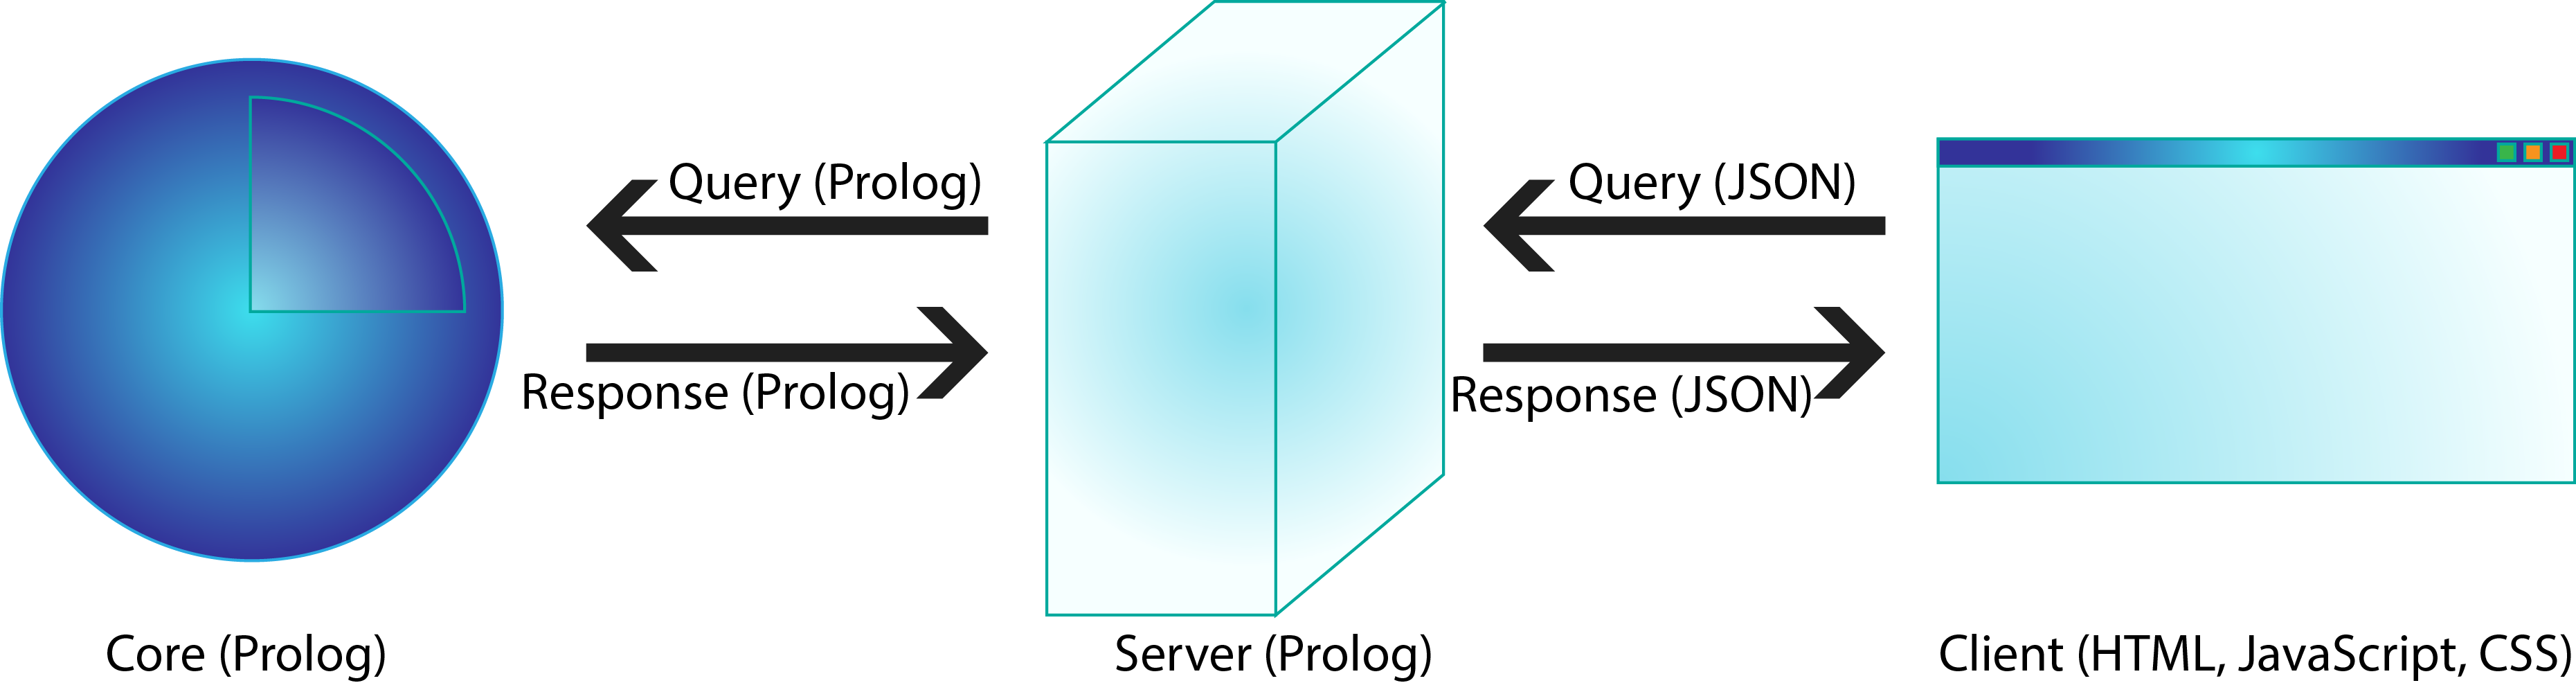
\includegraphics[scale=0.5]{img/system-diagram.png}}
\caption{The high-level system architecture for the chosen solution\label{fig:archdiag}}
\end{figure}

\subsection{Core}
The first (and arguably most important) part is the actual algorithms and code written to explore Argumentation Logic (henceforth referred to as "core"). The core is written entirely in Prolog, a procedural declarative programming language frequently used in the fields of artificial intelligence, logic and theorem proving. 

Prolog was chosen as the implementation language because it often leads to clean and concise code. Concise code arguably leads to fewer bugs, something very important to this project, as soundness is mandatory. Prolog offers pattern matching, backtracking and unification, making it ideal for creating a theorem proving system.

The Prolog language has many implementations, out of which \href{http://www.swi-prolog.org/}{SWI-Prolog}\footnote{http://www.swi-prolog.org/} was chosen because it is very fast and reliable, open-source and has a large array of helpful libraries and a large community.

\subsection{Server}
The second part of the project is the server. The server is used to load the core, and then serve HTTP (JSON) requests from the client by querying the core and replying with the results.

The server is written in Prolog as well. This has the obvious advantage of interoperability between the core and itself. The core's code (predicates) are loaded as part of the server's code and are used directly, and thus no middleware is required for the communication between the two parts.

The Prolog flavor used for the server is SWI-Prolog, which provides an \href{http://www.swi-prolog.org/pldoc/doc_for?object=section(\%27packages/http.html\%27)}{HTTP package}\footnote{http://www.swi-prolog.org/pldoc/doc\_for?object=section(\%27packages/http.html\%27)} that can set up and run a server with just a few lines of code. This virtually eliminated testing of this part of the project.

The server has exactly two responsibilities:

\begin{itemize}
\item
to serve files needed for the client to run - this includes HTML, JavaScript and CSS files
\item
to respond to requests by converting the JSON requests to Prolog, querying the core, converting the results back to JSON and replying to the client
\end{itemize}

The server is discussed in further detail in \autoref{chap:server}.

\subsection{Client}
The third and final part of the project is the client. The client serves as a front-end to the core, providing a helpful GUI as an alternative to the Prolog (interpreter's) command-line interface. It aims to provide useful facilities such as storage, importing and exporting of proofs and other data, syntax checking and so on.

The client consists of HTML, JavaScript and CSS files that are mainly served by the Prolog server. HTML 5 and JavaScript have become a very powerful combination that allow fast creation of elegant graphical interfaces, with many libraries available for free, making them a natural choice for a GUI.

The client is discussed in further detail in \autoref{chap:client}.

\section{Justification of Solution Architecture}
There are several advantages in splitting the project as mentioned in \autoref{sec:solarch}. However, as with any implementation, there are a few disadvantages as well. The pros and cons are discussed in this section.

\subsection{Advantages of Chosen Architecture}
The focus of the design is modularity and reusability. 

By completely detaching the core as a separate, self-contained module, testing becomes easier and more manageable. The responsibilities of this module become clearer. Since the core is completely detached, it can be run as-is, on the Prolog interpreter command-line just by itself, or it can be attached to a completely different program or GUI implementation or used in a different context.

The server can be swapped with a different implementation if required. This particular implementation is very small, largely due to the nature of the SWI-Prolog HTTP package that allows for a quick set-up of a webserver. The server currently has two responsibilities:

\begin{itemize}
\item
to serve files needed for the client to run - this includes HTML, JavaScript and CSS files
\item
to respond to requests by converting the JSON requests to Prolog, querying the core, converting the results back to JSON and replying to the client
\end{itemize}

An alternate setup can have this server respond only to requests and have a different, finely-tuned server (such as Apache) handle the load-balancing and HTTP requests of the clients. This webserver chaining is similar to how the SWI-Prolog website works at the time of writing - there is an exposed Apache server that redirects requests to a SWI-Prolog server hidden from the outside world. 

Since the project consists of a server and an HTML client, it can readily be hosted online and made available to the public. This way, a wider audience can be reached more quickly, which can result to valuable feedback.

The client is written in HTML, JavaScript and CSS, making it a web application. Advantages of web applications are fast, easy and transparent (to the user) updates, not requiring the user to re-download or update any software and cross-platform compatibility and hence larger availability. Web applications are ideal for incremental improvement, as a consequence of the previous advantages, and since this is largely a research project, in the future, it will be easier for features to be added as they are discovered. Finally, web applications integrate very well with other server-side services such as database access and account management, so the project can easily be extended in the future to support sharing of data and content via user accounts on the server.

\subsection{Disadvantages of Chosen Architecture}
As with every design, there are some drawbacks as well. There is some unavoidable duplication in data structures as different languages are used for the core and the client (Prolog vs JavaScript), and each language has to store and represent the data in some way. Some extra work is needed in order to keep the three parts of the system as modular as possible. Effort has to be made in synchronizing the different parts of the system when external interfaces are changed. For example, if the server is altered to accept a different data structure for the requests, then the client has to be update to provide requests that use the new data structure required by the server. Fortunately, internal changes (for example adding extra predicates or features to the core, adding extra UI elements to the client or revamping the GUI, or optimizing any of the three parts of the system) do not affect each module.

There are some disadvantages that come with web applications as well, but some of them fortunately do not apply to this system. Compatibility and performance issues (compared to native applications) are some of the common problems with web interfaces. Since the server does the heavy lifting the client is left with the responsibility of running the a simple GUI, ruling out any potential issues with performance. Every effort is made to make the Client adhere to standards, reducing the chances of running into compatibility issues with the browser. The main disadvantage however is the need for constant connection to the server. Unless the server is run locally, the client cannot be used as all calculations take place server-side.

\subsection{Structure of Remainder of Report}
The core implementation as well as the findings of this project are discussed in chapters TODO to TODO. An overview of the different features implemented in the core can be found in \autoref{chap:coreoverview}. The server implementation is discussed in more detail in \autoref{chap:server}. The client is discussed in \autoref{chap:client}. The evaluation of this project can be found in \autoref{chap:eval}, and finally, a conclusion is drawn based on the evaluation in \autoref{chap:chiliconclusion}. A full code listing for the core can be found in the Appendix (TODO).

\chapter{Core Functional Overview}
\label{chap:coreoverview}
The core is made of different predicates or procedures that work together in order to provide an ecosystem of functions that can be used to create and manipulate natural deduction proofs and arguments. \autoref{fig:funcmap} provides a functional map that illustrates the different procedures as well as the data flow around them.

\begin{figure}[ht]
\centerline{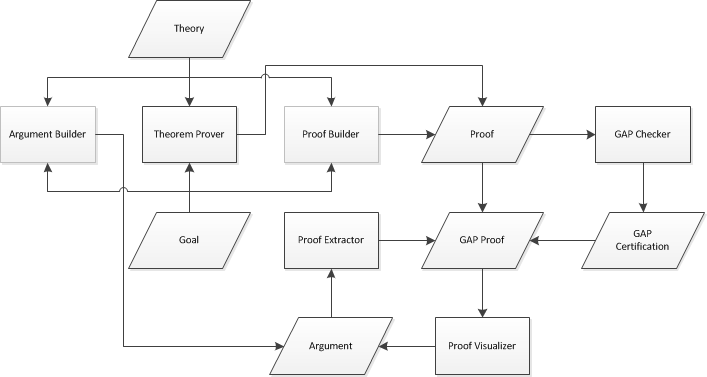
\includegraphics[scale=0.85]{img/functional-map.png}}
\caption{The high-level functional map for the core\label{fig:funcmap}}
\end{figure}

The main procedures involved are the following:
\begin{itemize}
\item
Theorem Prover (\autoref{chap:prover}): the theorem proof system provides proofs for the given theory and goal
\item
GAP Checker (\autoref{chap:gapcheck} and \autoref{chap:gapx}): the Genuine Absurdity Property checker takes a proof and succeeds if the given proof indeed follows the property
\item
Proof Visualizer (\autoref{chap:viz}): the proof visualization predicate takes a proof that follows the Genuine Absurdity Property and returns an argument that can be used to visualize the given proof
\item
Proof Extractor (\autoref{chap:extractor}): this predicate can take an argument (a visualization of a proof) and extract a proof from it
\end{itemize}

In addition to the core module predicates, there are a few client features that can still provide data that can be used by the core modules listed above. These are:
\begin{itemize}
\item
Proof Builder (\autoref{chap:proofbuilder}): provides a method of allowing the user to construct a particular proof
\item
Argument Builder(\autoref{chap:argbuilder}): provides a method of allowing the user to construct an argument 
\end{itemize}

\chapter{Theorem Proving System}
\label{chap:prover}
The first step in approaching this project is to build a theorem prover or a proof search system capable of generating proofs given a set of theory and a goal. Most existing implementations of such software use a different proof theory system (other than natural deduction) in order to generate proofs. Natural deduction, as discussed in \autoref{subsec:nnd}, is not the favorite choice for creating proofs. There are still however, a few implementations of a natural deduction theorem prover, but they did not meet all the requirements of this project and therefore were not suitable to use.

Different natural deduction provers use different sets of rules, some of which are derived. There are different styles of natural deduction as well, for example the Gentzen style that looks like sequent calculus where proofs following this format resemble trees, and the Fitch style natural deduction which resembles the format used in this paper. 

Apart from these variations, the ability to turn off a few rules, such as the Reductio ad Absurdum rule (and the derived "proof by contradiction" rule which combines a Reductio ad Absurdum rule and a $\neg E$ rule), in order to enable $\vdash_{MRA}$ (or $\nvdash_{MRA}$) proving used by the Genuine Absurdity Property (\autoref{chap:gapcheck}).

The theorem prover should also be flexible enough so that it can be used to stitch together sub-proofs in order to form a larger proof as required by the proof extraction algorithm discussed in \autoref{chap:extractor}.

\section{Ruleset Used}
The implementation tries to approach the proof both backwards (from the bottom up) and forwards (from the top down). Several backwards and forwards rules have been implemented. Backwards rules try to close the gap between the theory and the goal from the bottom, and they are the ones that complete goals in order to finish the proof. The forwards rules are there in order to break down complicated formulas that have already been derived so that the backwards rules can complete their work. The forwards rules do not progress the proof in the sense that they never deal with the goal. They just provide simpler formulas that can be of use to the backwards rules.

The implementation was partly modeled after (or at the very least inspired by) the Carnegie Mellon Proof Tutor (introduced in \autoref{subsec:carnage}, the full paper is \citep{siegfried}). However, the implementation follows a Fitch-style natural deduction. There are also explicit rules for contradiction. No distinction exists between the available assumptions $\alpha$ and derivable (using elimination rules) context $\beta$. Thus the whole context $\alpha\beta$ will be referred to as $\kappa$. In addition, instead of having one goal at a time, there can be several. Thus for the implementation, $G$ (as used so far) is a list of goals, and $\gamma|G$ indicates the first goal in the list $\gamma$ and the tail of the list $G$. The same notation will be used as much as possible.

Listed below are the forward rules:

\begin{itemize}
\item
$\wedge E: \kappa?G, \phi_1\wedge\phi_2\in\kappa, \phi_i\notin\kappa \Rightarrow \kappa,\phi_i?G, i = 1\, or\, 2\, or\, both$

(this rule is the same as the one used in the Carnegie Mellon Proof Tutor)
\item
$\neg E: \kappa?G, \neg\neg\phi\in\kappa, \phi\notin\kappa \Rightarrow \kappa\phi?G$

(if a double-negated formula is in the context, add the sub-formula without the double negation)
\item
$\bot I: \kappa?G, \phi\in\kappa, \neg\phi\in\kappa, \bot\notin\kappa \Rightarrow \kappa,\bot?G$

(if two opposite formulas are in the context, add a contradiction)
\end{itemize}

None of the forward rules touches the goal(s). They just simplify derived conjunctions, double negations and add a contradiction if one can be established.

The backward rules are listed here:

\begin{itemize}
\item
$\checkmark: \kappa?\gamma|G, \gamma\in\kappa \Rightarrow \kappa?G$

(if the current goal is already derived, move on to the next)
\item
$\wedge I: \kappa?\gamma_1\wedge\gamma_2|G, \gamma_i\notin\kappa \Rightarrow \kappa?\gamma_i|G, i = 1\, or\, 2\, or\, both$

(if the goal is a conjunction, then prove whatever constituent parts are missing)
\item
$\bot E: \kappa?\gamma|G, \bot\in\kappa \Rightarrow \kappa?G$

(anything can be derived if a contradiction has already been established)
\item
$\rightarrow I: \kappa?\gamma_1\rightarrow\gamma_2|G \kappa,\gamma_1?\gamma_2, \kappa?G$

(this rule is the same as the one used in the Carnegie Mellon Proof Tutor)
\item
$\neg I: \kappa?\neg\gamma|G \Rightarrow \kappa,\gamma?\bot, \kappa?G$

(this rule is the same as the one used in the Carnegie Mellon Proof Tutor)
\item
$\rightarrow E: \kappa?G, \phi_1\rightarrow\phi_2\in\kappa \Rightarrow \kappa?\phi_1, \kappa,\phi_2?G$

(this rule lies in between the forward and backward rule category, since it does not consume any of the goals, but it does however require that $\phi_1$ be proven; what it says is try to prove the first part of the implication, and hence add the second part to the context before moving on to prove the goal)
\item
$PC: \kappa?\gamma|G, \gamma\neq\bot \Rightarrow \kappa,\neg\gamma?\bot, \kappa?G$

(proof by contradiction, implemented as a combination of $\neg I$ and $\neg E$ rules - this rule is the same as the one used in the Carnegie Mellon Proof Tutor)

\item
$\bot IE: \kappa?\gamma|G, \bot\notin\kappa, \neg\phi\in\kappa \Rightarrow \kappa?\phi, \kappa?G$

(take any negated formula and try to prove its positive subformula, essentially proving a contradiction; the goal is then vacuously true - composite rule implemented using $\bot I$ and $\bot E$ rules)
\end{itemize}

\section{Propositional Logic Format}
This implementation uses Prolog predicates in order to specify the different logic constructs. \autoref{fig:prolol} summarizes these predicates.

\begin{figure}[tph]
\begin{center}
\begin{tabular}{|l|l|}
\hline
Logic Construct & Prolog Term Used By Implementation\\
\hline
Conjunction & \lstinline$and(A, B)$\\
\hline
Disjunction & \lstinline$or(A, B)$\\
\hline
Implication & \lstinline$implies(A, B)$\\
\hline
Negation & \lstinline$n(A, B)$\\
\hline
Contradiction & \lstinline$falsity$\\
\hline
\end{tabular}
\end{center}
\caption{The Prolog constructs accepted and used by the theorem prover\label{fig:prolol}}
\end{figure}

As an example, consider the formula $a\wedge b\rightarrow\neg c$. This would be represented by the following data structure: \lstinline$implies(and(a, b), n(c))$.

\section{High-Level Description of Implementation}
The theorem prover was built to be quite modular and offers both high-level and low level predicates. For the most part, high-level predicates are enough to cover the needs of the different algorithms created to check for the Genuine Absurdity Property, or to aid the building of an argument. It was necessary however at some point to use the low-level plumbing of the theorem prover in order to stitch together specific proofs generated with more complicated context for the proof extractor algorithm.

A summary of the high-level predicates is given below:

\begin{itemize}
\item
\lstinline$prove(Givens, Goal, Proof)$: The user supplies the theory as a list of formulas and a goal as a singleton list of one formula that needs to be proven. The predicate returns with \lstinline$Proof$ bound to one possible proof. The \lstinline$prove/3$ predicate offers choice-points, with each choice-point offering one solution. All solutions for the given theory and goal can be acquired by executing a \lstinline$findall/3$ predicate like this: \lstinline$findall(Proof, prove([and(a,b)], [and(b,a)], Proof), AllProofs)$ with \lstinline$AllProofs$ containing all the proofs what prove the goal.
\item
\lstinline$proveMRA(Givens, Goal, Proof)$: This works in the same way as \lstinline$prove/3$, but it makes no use of the $\neg I$ and (derived) proof by contradiction rules. This can be used to check for the Genuine Absurdity Property or to help build arguments (\autoref{chap:argbuilder}).
\item
\lstinline$provable(Givens, Goal, MRA, Verdict)$ This works similarly to the above predicates, but instead of supplying a proof upon return, it only responds with a \lstinline$yes$ or \lstinline$no$ atom, depending on whether the supplied goal can be proven using the given theory. The \lstinline$MRA$ field takes a \lstinline$yes$ or \lstinline$no$ atom and defines whether $\vdash$ or $\vdash_{MRA}$ is used to prove the goal (ie whether $\neg I$ and proof by contradiction can be used). This predicate always finishes without any choice-points.
\end{itemize}

The above predicates handle the burden of converting the input into steps (see \autoref{sec:outputformat}), and then calling the necessary low-level predicate to fire off the process. The theorem prover however was built to work even if the user chooses to execute a low-level predicate instead (assuming correct input was given). This enables the user to, for example, start a proof with the application of a particular rule. The available low-level predicates are summarized below:

\begin{itemize}
\item
\lstinline$backwardProve(MRA, Steps, Context, Extras, Goals, Proof)$: This predicate starts the backwards proving of the goal(s), by trying to use any of the available rules depending on whether \lstinline$MRA$ is set to \lstinline$yes$ or \lstinline$no$. The steps parameter contains the actual steps of the current context, and the context parameter specifies additional context (that was inherited by ancestors).
\item
\lstinline$check(MRA, Steps, Context, Extras, Goals, Proof)$
\item
\lstinline$falsityI(MRA, Steps, Context, Extras, Goals, Proof)$
\item
\lstinline$andI(MRA, Steps, Context, Extras, Goals, Proof)$
\item
\lstinline$impliesI(MRA, Steps, Context, Extras, Goals, Proof)$
\item
\lstinline$notI(MRA, Steps, Context, Extras, Goals, Proof)$
\item
\lstinline$forward(MRA, Steps, Context, Extras, Goals, Proof)$
\item
\lstinline$falsityIE(MRA, Steps, Context, Extras, Goals, Proof)$
\item
\lstinline$impliesE(MRA, Steps, Context, Extras, Goals, Proof)$
\item
\lstinline$proofByContradiction(MRA, Steps, Context, Extras, Goals, Proof)$
\end{itemize}

All of the backward rules are available to be called immediately by the user, and they will generate a proof with an initial application of that rule. If given the right input the rules will take care of the rest of the proof as well and come back with a complete proof of the goal(s). The "forward rule" is a "rule" that tries to apply all the forward rules and call \lstinline$backwardProve/6$ again.

\section{Output Format}
\label{sec:outputformat}
The output of the theorem prover is a Prolog list of steps or boxes. A step is defined as \lstinline$step(Derivation, Reason, LineNumber)$ where \lstinline$Derivation$ is a formula using Prolog terms, the reason is a list with at least one element inside, and a line number is just a non-negative number that is used to uniquely identify the step (so that other steps' reasons can reference that step). A box contains sub-proofs (that begin with a hypothesis) that are essentially lists of more steps and boxes (defined as \lstinline$box(SubProof)$).

The reason is a list where the first element is the name of the justification for the derivation in that step as a Prolog atom. Some reasons are required to reference other steps in the proof in order to fully justify how the formula in the step was derived. For example, for an application of the $\wedge I$ rule, both subformulas of the conjunction need to be referenced by including the numbers of the steps containing those subformulas in the list.

Reasons include the natural deduction rules specified before. They also contain a few more reasons such as \lstinline$hypothesis$ to indicate a hypothesis or \lstinline$given$ to indicate a part of the theory. \autoref{fig:output} lists the reasons and the number of reference line numbers required by each reason.

\begin{figure}[tph]
\begin{center}
\begin{tabular}{|l|l|l|}
\hline
Reason Prolog Term & Reference Line Numbers & Description\\
\hline
\lstinline$check$ & 1 & Reiteration of an existing formula\\
\hline
\lstinline$andI$ & 2 & $\wedge I$ from subformulas on referenced lines\\
\hline
\lstinline$andE$ & 1 & $\wedge E$ from conjunction on referenced line\\
\hline
\lstinline$impliesI$ & 2 & $\rightarrow I$ from subformulas on referenced lines\\
\hline
\lstinline$impliesE$ & 2 & $\rightarrow E$ from implication and its first part\\
&& indicated by referenced lines\\
\hline
\lstinline$notI$ & 2 & $\neg I$ from hypothesis and contradiction on \\
&& referenced lines\\
\hline
\lstinline$notE$ & 1 & $\neg E$ from double-negated formula on referenced\\
&& line\\
\hline
\lstinline$falsityI$ & 2 & $\bot I$ from opposite formulas on referenced lines\\
\hline
\lstinline$falsityE$ & 1 & $\bot E$ from contradiction indicated by referenced\\
&& line\\
\hline
\lstinline$hypothesis$ & 0 & a hypothesis put forth\\
\hline
\lstinline$given$ & 0 & part of the theory\\
\hline
\end{tabular}
\end{center}
\caption{The Prolog constructs accepted and used by the theorem prover\label{fig:output}}
\end{figure}

The list contains elements in the opposite order as one would read a proof on paper. That is, the first element in the list will be the conclusion of the proof, and the last elements of the list will be the givens (theory) that are always located at the beginning of the proof. The reason as to why the proof is in the opposite order is that Prolog offers a concise way to append elements to a list, and the backward rules tend to add steps to the end of the proof instead of the beginning. Therefore the proof is build backwards in a sense. Predicates are provided that can flip the proof as necessary and are indeed used when responding to the client with generated proofs from the theorem prover.

As an example of the output generated by the theorem prover, consider the proof and its corresponding data structure as generated by the theorem prover in \autoref{fig:ndvstp}.

\begin{figure}[htp]
\begin{minipage}[c]{.35\linewidth}
\[\vbox{\offinterlineskip\halign{
&\tabskip=1.5em#\strut&$#$\hfil\tabskip=1em&\hfil$#$\tabskip=0em\cr
%
1&\neg(\alpha\wedge\beta)&\mbox{given}\cr
2&\neg(\alpha\wedge\neg\beta)&\mbox{given}\cr
3&\neg\beta&\mbox{given}\cr
%
\multispan3\vbox{\halign{
\vrule#&&\hskip.1em\tabskip=1em#\strut&$#$\hfil\tabskip=1em&\hfil$#$\hskip0.1em\tabskip=0em&\vrule#\cr
\noalign{\hrule}
%
&4&\alpha&\mbox{hypothesis}&\cr
%
&\multispan3\,\vbox{\halign{
\vrule#&&\hskip.1em\tabskip=1em#\strut&$#$\hfil\tabskip=1em&\hfil$#$\hskip0.1em\tabskip=0em&\vrule#\cr
\noalign{\hrule}
%
&5&\beta&\mbox{hypothesis}&\cr
&6&\alpha\wedge\beta&\wedge I(4,5)&\cr
&7&\bot&\bot I(1,6)&\cr
%
\noalign{\hrule}}}\,&\cr
%
&8&\neg\beta&\neg I(5,7)&\cr
&9&\alpha\wedge\neg\beta&\wedge I(4,8)&\cr
&10&\bot&\bot I(2,9)&\cr
%
\noalign{\hrule}}}\,\cr
%
11&\neg\alpha&\neg I(4,10)\cr
}}\]
\end{minipage}%
\begin{minipage}[c]{.65\linewidth}
\begin{lstlisting}
[
	step(n(a), [notI, 4, 10], 11),
	box([
		step(falsity, [falsityI, 2, 9], 10),
		step(and(a, n(b)), [andI, 4, 8], 9),
		step(n(b), [notI, 5, 7], 8),
		box([
			step(falsity, [falsityI, 1, 6], 7),
			step(and(a, b), [andI, 4, 5], 6),
			step(b, [hypothesis], 5)
		]),
		step(a, [hypothesis], 4)
	]),
	step(n(b), [given], 3),
	step(n(and(a, n(b))), [given], 2),
	step(n(and(a, b)), [given], 1)
]
\end{lstlisting}
\end{minipage}
\caption{A natural deduction proof and the corresponding output from the theorem prover\label{fig:ndvstp}}
\end{figure}

\section{Remarks}
\label{sec:tpeval}

\subsection{Correctness}
In terms of correctness, the theorem prover should be both sound and complete regarding its implemented logic constructs. It uses the Carnegie Mellon Proof Tutor as a starting point which is itself sound and complete. The deviations do not lead to unsound proofs, and completeness should still be maintained. As with any piece of software however, there exists a possibility of errors. No software is perfect, and hence the theorem prover may suffer from bugs. In order to be completely sure that the software works, formal verification methods should be employed. However, such methods take too much time and require a great deal of effort. The theorem prover is critical to the project, however it is not its main focus. The main focus remains the Argumentation Logic. In place of formal verification methods, testing has been applied in order to try and eliminate as many errors as possible and to provide a good starting point for when upgrades or other changes are made to the current version of the prover.

In order to test the implementation \href{http://www.swi-prolog.org/pldoc/package/plunit.html}{plunit}\footnote{http://www.swi-prolog.org/pldoc/package/plunit.html} was used as the unit test framework of choice. Thankfully, the team behind SWI-Prolog created this unit test framework that works quite well with their Prolog implementation. Several tests were laid out both trying to test that the theorem prover can prove goals that are provable (given the necessary theory) and that it cannot (and should not) prove goals that can't be reached (given again the necessary theory). For the sake of brevity, the test suites will not be included in the report, but are available in the source code of the project.

\subsection{Performance, Pruning and Optimization}
The theorem prover works well in general. It does sometimes seem to get slow on complicated theories and proofs that exhibit a very large search space. The purpose of the theorem prover is to be able to provide "all" proofs that prove a goal given a theory. However it is very difficult to exactly specify what "all" means. Obviously there can be infinite proofs for any goal given to the theorem prover (at the very least, the theorem prover could take any atom from the theory and start building an infinite conjunction chain, chaining together that very atom to produce infinite proofs). Instead, the theorem prover tries to produce all (close to) normal proofs. This means that it tries not to take detours by imposing restrictions in its ruleset (see restricted rules in \autoref{subsec:carnage}). This ensures that a finite set of proofs can be generated for a particular goal. Still, that set could be very large, as any (allowed) permutation in a Fitch-style natural deduction proof can be considered a completely different proof. 

The next step could be to prune the search space and drop proofs that are not good. However, ambiguity is faced when it comes to defining "good" proofs. Consider the proofs in \autoref{fig:topruneornottoprune} for defining the measure "good":

\begin{figure}[htp]
\begin{minipage}[c]{.5\linewidth}
\[\vbox{\offinterlineskip\halign{
&\tabskip=1.5em#\strut&$#$\hfil\tabskip=1em&\hfil$#$\tabskip=0em\cr
%
1&\alpha&\mbox{given}\cr
2&\alpha&\checkmark\cr
}}\]
\end{minipage}%
\begin{minipage}[c]{.5\linewidth}
\[\vbox{\offinterlineskip\halign{
&\tabskip=1.5em#\strut&$#$\hfil\tabskip=1em&\hfil$#$\tabskip=0em\cr
%
1&\alpha&\mbox{given}\cr
%
\multispan3\vbox{\halign{
\vrule#&&\hskip.1em\tabskip=1em#\strut&$#$\hfil\tabskip=1em&\hfil$#$\hskip0.1em\tabskip=0em&\vrule#\cr
\noalign{\hrule}
%
&2&\neg\alpha&\mbox{hypothesis}&\cr
&3&\bot&\bot I(1,2)&\cr
%
\noalign{\hrule}}}\,\cr
%
4&\neg\neg\alpha&\neg I(2,3)\cr
5&\alpha&\neg E(4)\cr
}}\]
\end{minipage}

\caption{Pruning could potentially trim proofs of potential importance regarding Argumentation Logic\label{fig:topruneornottoprune}}
\end{figure}

One could argue that the second proof is unnecessary and could be trimmed since it is just a detour from the first proof. However, it is sometimes these scenic routes that are the best routes, and in Argumentation Logic it is no different. The proof on the right happens to follow the Genuine Absurdity Property and can therefore be visualized (see \autoref{chap:viz}). If it were to be pruned, the remaining results would be of little use.

It is therefore necessary to devise pruning algorithms and optimizations that do not reduce the amount of generated proofs that follow the Genuine Absurdity Property, as they are the most valuable proofs. Argumentation Logic-compatible pruning and optimizations remain part of future work.

One optimization that was implemented that does not change the number of generated proofs is an optimization that grades all of the negated formulas in the current context of a proof, when the theorem prover decides to use the $\bot IE$ rule. This rule gathers all negated formulas and tries to prove their positive sub-formulas in an attempt to prove the goal using a contradiction. The optimization tries to find the number of subformulas of the positive sub-formula that have not been proven yet. Then it rates each negated formula with a number, which is the number of to-be-proven sub-formulas. The theorem prover then orders the negated formulas according to their rating and attempts to use the most promising negated formula first; ie the one that has the fewest sub-formulas remaining to be proven. This is most of the times a great heuristic that guides the search but does not prune it in any way. 

\subsection{Improvements and Extensions}
As mentioned before, one of the improvements that could be made is to increase the performance of the theorem prover. This could involve either a more efficient implementation altogether, or the introduction of optimizations with regards to the search space or pruning of (paths that lead to) "bad" proofs. The latter would involve defining explicitly what "bad" proofs are with respect to Argumentation Logic.

The theorem prover currently does not support disjunction. This was done in order to save time that was allocated to extending the Genuine Absurdity Property definition. Since this property does not make use of the implication and disjunction logic constructs, supporting them may be regarded as unnecessary. However, even for the sake of completeness over all logic constructs, disjunction could be introduced to the supported connectives.

\chapter{Checking for Genuine Absurdity Property}
\label{chap:gapcheck}
Recall from \autoref{subsec:gap} that for a RAND derivation, $T\cup\{\phi\}\cup\{\phi_1, ..., \phi_k\}\cup\{\neg\psi_1, ..., \neg\psi_l\}\vdash_{MRA}\bot$, where $k, l \geq 0$ and

\begin{itemize}
\item
$\phi$ is the hypothesis of this derivation
\item
$\phi_i$ are the hypothesis of parent derivations that this derivation has access to and can make use of
\item
$\psi_i$ are the hypotheses of the children derivations, the negations of which can be used by this derivation
\end{itemize}

Moreover, recall that the Genuine Absurdity Property forms a kind of relevance by requiring that the hypothesis $\phi$ is necessary for the derivation of the contradiction. In other words, without $\phi$, a contradiction cannot be established. In formal notation, this would be described as

\[T\cup\{\phi_1, ..., \phi_k\}\cup\{\neg\psi_1, ..., \neg\psi_l\}\nvdash_{MRA}\bot\]

Recall, further, that the Genuine Absurdity Property is a recursive property in that any sub-derivations of an application of the Reductio ad Absurdum rule must also follow this property, and finally, that this property is defined only over proofs using conjunction and negation only. Note once again, that the set $\{\phi_1, ..., \phi_k\}$ includes all ancestor hypotheses copied from outside the sub-derivation.

\section{Short Description of Algorithm}
In a nutshell, the algorithm for checking for the Genuine Absurdity Property traverses the proof and keeps track of ancestor hypotheses and child hypotheses as well as the theory given initially. At the beginning the algorithm checks that the given proof is a RAND proof and that it only contains conjunctions and negations of atoms. In addition, it checks that the proof does not make use of any shortcuts. Those are dealt in the extended version of the Genuine Absurdity Property discussed in \autoref{chap:gapx}.

The ancestor hypotheses are tracked by crawling the proof backwards from each line in the sub-derivation, using the justifications as (potentially forking) paths to guide the search. The child hypotheses are tracked by reading the hypothesis at the top of each sub-derivation and negating it.

Before reaching the end of the current application of the $\neg I$ rule, each sub-derivation is also checked that it follows the Genuine Absurdity Property by calling the algorithm again recursively.

At the end of each application of the Reductio ad Absurdum rule the Genuine Absurdity Property is checked by asking the theorem prover in \autoref{chap:prover} to try and prove a contradiction using the given theory, and the ancestor and (negations of the) child hypotheses. That is, we ask the prover to prove that $T\cup\{\phi_1, ..., \phi_k\}\cup\{\neg\psi_1, ..., \neg\psi_l\}\vdash_{MRA}\bot$. If that succeeds, then we know that a contradiction could have been reached without the use of the hypothesis in the current application of the Reductio ad Absurdum rule, thus making the proof not follow the property under check.

\section{Details of Implementation}
The overall algorithm is split into four stages. The first stage involves checking whether the given proof is a RAND proof. That is, apart from the theory, the proof should only contain an application of the Reductio ad Absurdum rule on the top level. The second stage involves checking whether the given proof has formulas consisting of only conjunction and negation. The third stage checks that the proof does not make any use of the substitution rule. The fourth and final stage is the actual check which verifies the Genuine Absurdity Theory.

\begin{lstlisting}[caption={Genuine Absurdity Property top level predicate},label=lst:gaptoppred]
% Checks that the given proof follows the GAP property
% Gap checker assumes valid propositional logic proofs
checkGAP(Proof) :- 
	reverse(Proof, RevProof), 
	checkRAND(RevProof), !,
	checkRestrictedRules(RevProof), !,
	getTheoryAndRevBox(RevProof, Theory, RevBox), !,
	checkRestrictedTheory(Theory), !,
	checkPureND(Theory, RevBox), !,
	checkGAP(Theory, _, [], [], RevBox), !.
\end{lstlisting}

\autoref{lst:gaptoppred} shows the top-level predicate where the four stages (checks) can be seen at line 5 for RAND proof, lines 6 and 7 for the restricted use of propositional logic, line 9 for the lack of shortcuts and finally line 10 for the actual check for the definition of the Genuine Absurdity Property. The format of the proof is the same as that output by the theorem proving algorithm in \autoref{chap:prover}. The four stages are further discussed below.

\subsection{Checking for RAND Proof}
The format of a RAND proof is the following: first, there may or may not be a few steps containing the theory. These are steps that are justified with "given". Following should be a box, and finally, there should be either the goal (derived using the box), or the double negation of the goal (derived using the box) and the goal (derived by $\neg E$).

\begin{lstlisting}[caption={Checking whether a proof is a RAND proof},label=lst:gaprandcheck]
% Checks to see if this proof is a RAND proof to start with
% A RAND proof is of the form: [givens]*, [box], ([step:notE, step:notI]||[step:notI])
checkRAND(Proof) :- checkRAND(givens, Proof).
checkRAND(givens, [box(_)|Proof]) :- checkRAND(box, Proof).
checkRAND(givens, [step(_, [given], _)|Proof]) :- checkRAND(givens, Proof).
checkRAND(box, [step(_, [notI|_], _)]).
checkRAND(box, [step(_, [notI|_], _), step(_, [notE, _], _)]).
\end{lstlisting}

On line 3 of \autoref{lst:gaprandcheck} the \lstinline$checkRAND/1$ predicate starts the check by calling \lstinline$checkRAND/2$ and specifying that it is at the "givens" stage (ie that it is now going through the theory). Line 5 unwinds the proof by iterating through the theory until a box is found and picked up by line 4, which marks the "box" stage. Finally, lines 6 and 7 check that the last step of the proof is the conclusion, which might be preceded by its double negation (which is the product of the $\neg I$ rule and the box before.

\subsection{Checking for Restricted Formulas}
It suffices to check in a proof that the theory is constructed using conjunction and negation, and that the rules applied subsequently belong to the set of $\{\wedge I, \wedge E, \neg I, \neg E, \bot I, \bot E\}$.

\begin{lstlisting}[caption={Checking whether a proof uses only conjunction and negation},label=lst:gaprestrictedcheck]
% Checks to see if the proof consists of ruleset defined over argumentation logic
validRules([andI, andE, notI, notE, falsityI, falsityE, given, check, hypothesis]).
checkRestrictedRules([]).
checkRestrictedRules([step(_, [Reason|_], _)|Proof]) :- 
	validRules(ValidRules), 
	m2(Reason, ValidRules), 
	checkRestrictedRules(Proof).
checkRestrictedRules([box(SubProof)|Proof]) :-
	checkRestrictedRules(SubProof),
	checkRestrictedRules(Proof).
checkRestrictedTheory([]).
checkRestrictedTheory([Given|Theory]) :-
	checkRestrictedFormula(Given),
	checkRestrictedTheory(Theory).
checkRestrictedFormula(X) :- 
	atom(X).
checkRestrictedFormula(and(X, Y)) :-
	checkRestrictedFormula(X),
	checkRestrictedFormula(Y).
checkRestrictedFormula(n(X)) :-
	checkRestrictedFormula(X).
\end{lstlisting}

The predicate \lstinline$checkRestrictedTheory/1$ as shown in \autoref{lst:gaprestrictedcheck} looks at the theory contained in the proof and makes sure that it consists only of atoms, conjunctions and negations. The predicate \lstinline$checkRestrictedRules/1$ shown in \autoref{lst:gaprestrictedcheck} again ensures that rules that could potentially introduce a new construct (such as implication or disjunction) are not used. This predicate probes nested boxes as well so that the entire proof is covered. The predicate \lstinline$m2/2$ on line 6 acts as an alias to the standard \lstinline$member/2$ Prolog predicate.

\subsection{Ensuring the Lack of Substitution}
This stage looks at the line number references that the steps inside a derivation address, and checks that all line numbers either refer to steps inside the current context, theory, or parent hypotheses. Any other references are considered extraneous.

\begin{lstlisting}[caption={Checking whether a proof uses any shortcuts},label=lst:gapsubcheck]
% Checks to see if this proof does not make references to external derivations
checkPureND(Theory, Proof) :-
	length(Theory, TheoryLength),
	checkPureND(TheoryLength, _, Proof, Proof).
checkPureND(_, _, [], _) :- !.
checkPureND(L, _, [step(_, [hypothesis], LN)|Proof], WholeProof) :-
	!, checkPureND(L, LN, Proof, WholeProof).
checkPureND(L, LN, [step(_, [_|ReasonLines], _)|Proof], WholeProof) :-
	forall(m2(RL, ReasonLines), (RL >= LN; RL < L; getStep(RL, WholeProof, step(_, [hypothesis], RL)))),
	checkPureND(L, LN, Proof, WholeProof).
checkPureND(L, LN, [box(BoxProof)|Proof], WholeProof) :-
	checkPureND(L, _, BoxProof, WholeProof),
	checkPureND(L, LN, Proof, WholeProof).
\end{lstlisting}

\autoref{lst:gapsubcheck} shows predicate \lstinline$checkPureND/2$ which takes the theory and the proof under examination. It measures the size of the theory, and passes this information along with the proof to \lstinline$checkPureND/4$. Line 7 makes a note of the line number of the hypothesis, which is the first step of each sub-derivation. Line 9 checks that all referenced steps by the line currently under consideration are either internal steps (bigger than the hypothesis line number measured by line 7 of the code) or point to the theory (any line references smaller than the length of the theory are considered acceptable as the theory always appears at the top of the proof), or that they point to a hypothesis (of an ancestor). The last clause of \lstinline$checkPureND$ makes sure that all sub-derivations are visited.

\subsection{Checking for Genuine Absurdity Property}
The final part of the algorithm deals with the definition of the Genuine Absurdity Property directly.

\begin{lstlisting}[caption={Checking whether a proof follows the Genuine Absurdity Property},label=lst:gapgapcheck]
% Checks for the actual GAP for each (sub)derivation in the proof
checkGAP(Theory, AncestorHypotheses, ChildHypotheses, SiblingHypotheses, [], _, _) :-
	a4(Theory, AncestorHypotheses, ChildHypotheses, SiblingHypotheses, Context),
	not(proveMRA(Context, [falsity], _)).
checkGAP(Theory, [], ChildHypotheses, SiblingHypotheses, [step(_, [hypothesis], HL)|Proof], WholeProof, _) :-
	!, checkGAP(Theory, [], ChildHypotheses, SiblingHypotheses, Proof, WholeProof, HL).
checkGAP(Theory, AncestorHypotheses, ChildHypotheses, SiblingHypotheses, [step(_, [_|Reason], _)|Proof], WholeProof, HL) :-
	getUsedHypotheses(Theory, Reason, WholeProof, HL, NewAncHypotheses, NewSibHypotheses),
	a2(NewSibHypotheses, SiblingHypotheses, NewSiblingHypotheses),
	a2(NewAncHypotheses, AncestorHypotheses, NewAncestorHypotheses),
	checkGAP(Theory, NewAncestorHypotheses, ChildHypotheses, NewSiblingHypotheses, Proof, WholeProof, HL).
checkGAP(Theory, AncestorHypotheses, ChildHypotheses, SiblingHypotheses, [box(BoxProof)|Proof], WholeProof, HL) :-
	checkGAP(Theory, [], [], [], BoxProof, WholeProof, _),
	BoxProof = [step(ChildHypothesis, [hypothesis], _)|_],
	(
		ChildHypothesis = n(X),
		NegatedChildHypothesis = X;
		
		NegatedChildHypothesis = n(ChildHypothesis)
	),
	checkGAP(Theory, AncestorHypotheses, [NegatedChildHypothesis|ChildHypotheses], SiblingHypotheses, Proof, WholeProof, HL).
\end{lstlisting}

The format of the proof passed in this predicate is the opposite of that output by the theorem prover in \autoref{chap:prover} in that the steps are in increasing order as one would read the proof on paper. This is due to the work of the \lstinline$getTheoryAndRevBox/3$ predicate called before the check as shown in \autoref{lst:gaptoppred}.

The clause on line 4 of \autoref{lst:gapgapcheck} makes a note of the location (line number) of the hypothesis. It is the one and only clause that Prolog chooses upon entering a new box (application of the Reductio ad Absurdum rule). All intermediate steps bear little significance in what they actually do, but it is very important to check what steps of the proof they refer to, and extract potential ancestor hypotheses. This is done by the clause on line 7, using \lstinline$getUsedHypotheses/6$, which returns the ancestor and sibling hypotheses used. The latter set will of course be empty and will not affect the check for the original definition. This is because it is known from the previous check for the lack of substitutions (shortcuts) that there are no references to external conclusions (sibling derivations).

Child proofs however must be checked for the Genuine Absurdity Property as well as this property is recursive. Line 7 takes that into account. It adds the hypothesis of the current context into the ancestor hypotheses of a new call to the \lstinline$checkGAP/7$ predicate (line 9). If the sub-derivation follows the property, the algorithm continues to add the negation of the sub-derivation hypothesis to the child hypotheses. 

At the end of the current context, when all the child hypotheses have been gathered and checked that they follow the property, the algorithm checks that the property holds for this context as well. This is done by the clause on line 2. The predicate \lstinline$a3/4$ ("append 3 lists") on line 3 merges the theory, ancestor hypotheses and child hypotheses gathered so far into one bundle, and calls for the theorem prover to try and prove a contradiction while purposely excluding the hypothesis of the current context from the bundle (line 4). That is, the theorem prover is given the task of proving $T\cup\{\phi_1, ..., \phi_k\}\cup\{\neg\psi_1, ..., \neg\psi_l\}\vdash_{MRA}\bot$. If it succeeds, then the Genuine Absurdity Theory does not hold. If it fails, then so far the property holds.

Line 8 scans the line references of intermediate steps in the current derivation to find references to sibling derivations. The scanning and gathering of referenced siblings is done by \lstinline$getUsedSiblingHypotheses/6$ which is shown in \autoref{lst:ancmining}.

\begin{lstlisting}[caption={Gathering of referenced ancestor derivations for the original Genuine Absurdity Property definition},label=lst:ancmining]
% Uses the line references to find referenced sibling derivations
getUsedHypotheses(_, [], _, _, [], []) :- !.
getUsedHypotheses(Theory, Reason, WholeProof, HL, NewAncHypotheses, NewSibHypotheses) :-
	length(Theory, L),
	findall(R, (m2(R, Reason), R < HL, R >= L), External),
	findall([H1, E1], (m2(E1, External), getStep(E1, WholeProof, step(H1, [notI|_], _))), HLN1),
	unzip(Hs1, LNs1, HLN1),
	subtract(External, LNs1, Rest1),
	findall([H2, E2], (m2(E2, Rest1), getStep(E2, WholeProof, step(H2, [hypothesis], _))), HLN2),
	unzip(Hs2, LNs2, HLN2),
	subtract(Rest1, LNs2, Rest2),
	findall(Reason2, (m2(R2, Rest2), getStep(R2, WholeProof, step(_, [_|Reason2], _))), Reasons),
	append(Reasons, Reasons2),
	getUsedHypotheses(Theory, Reasons2, WholeProof, HL, NewAncHypotheses2, NewSibHypotheses2),
	append(Hs1, NewSibHypotheses2, NewSibHypotheses),
	append(Hs2, NewAncHypotheses2, NewAncHypotheses).
	
unzip([], [], []).
unzip([L|Ls], [R|Rs], [[L,R]|Ps]) :- unzip(Ls, Rs, Ps).
\end{lstlisting}

The predicate \lstinline$getUsedSiblingHypotheses/6$ works by measuring the size of the theory in steps (line 4 of the code). Any line references smaller than this number indicate a reference to the theory (since the theory appears first in the proof, its line numbers are always smaller than the size of the theory in steps). When called, this predicate knows the line number of the hypothesis of the current derivation. Any reference to a line greater than (or equal to) the line number of the current hypothesis indicates an internal reference and can therefore be ignored. This filtering is done by line 5, that only gathers extraneous references that do not point to the theory. 

Out of these, all steps that are conclusions are filtered and stored (line 6). These constitute sibling conclusion references (indirectly, references to sibling hypotheses). Since the check performed by the \lstinline$checkPureND/2$ guarantees that there are no references to siblings, this line has no effect. This piece of code plays an important role in the extended version of the Genuine Absurdity Property discussed in \autoref{chap:gapx}.

The remaining extraneous references are checked whether they point to an ancestor hypothesis (line 9) and if that is the case, the hypothesis is stored. The remaining extraneous references are then recursively explored by lines 12-14 of the code until the recursion bottoms out. The extracted ancestor conclusions from the recursion at deeper levels are appended to the ones found in the current level of recursion and when the recursion bubbles back up, all ancestor hypotheses referenced by the examined step are returned. The sibling hypotheses returned when checking for the original definition of the property is just an empty list.

\section{Example Walkthrough}
This example will focus on the \lstinline$checkGAP/7$ predicate shown in \autoref{lst:gapgapcheck}. Consider a proof with theory $\{\neg(\beta\wedge\alpha), \neg(\alpha\wedge\gamma), \neg(\alpha\wedge\neg\beta\wedge\neg\gamma)\}$ and goal $\neg\alpha$. The proof is given below: 

\[\vbox{\offinterlineskip\halign{
&\tabskip=1.5em#\strut&$#$\hfil\tabskip=1em&\hfil$#$\tabskip=0em\cr
%
1&\neg(\beta\wedge\alpha)&\mbox{given}\cr
2&\neg(\neg\beta\wedge\gamma)&\mbox{given}\cr
3&\neg(\alpha\wedge\neg\beta\wedge\neg\gamma)&\mbox{given}\cr
%
\multispan3\vbox{\halign{
\vrule#&&\hskip.1em\tabskip=1em#\strut&$#$\hfil\tabskip=1em&\hfil$#$\hskip0.1em\tabskip=0em&\vrule#\cr
\noalign{\hrule}
%
&4&\alpha&\mbox{hypothesis}&\cr
%
&\multispan3\,\vbox{\halign{
\vrule#&&\hskip.1em\tabskip=1em#\strut&$#$\hfil\tabskip=1em&\hfil$#$\hskip0.1em\tabskip=0em&\vrule#\cr
\noalign{\hrule}
%
&5&\beta&\mbox{hypothesis}&\cr
&6&\beta\wedge\alpha&\wedge I(5,4)&\cr
&7&\bot&\bot I(1,6)&\cr
%
\noalign{\hrule}}}\,&\cr
%
&8&\neg\beta&\neg I(5,7)&\cr
%
&\multispan3\,\vbox{\halign{
\vrule#&&\hskip.1em\tabskip=1em#\strut&$#$\hfil\tabskip=1em&\hfil$#$\hskip0.1em\tabskip=0em&\vrule#\cr
\noalign{\hrule}
%
&9&\gamma&\mbox{hypothesis}&\cr
&10&\alpha\wedge\gamma&\wedge I(4,9)&\cr
&11&\bot&\bot I(2,10)&\cr
%
\noalign{\hrule}}}\,&\cr
%
&12&\neg\gamma&\neg I(9,11)&\cr
&13&\alpha\wedge\neg\beta&\wedge I(4,8)&\cr
&14&\alpha\wedge\neg\beta\wedge\neg\gamma&\wedge I(13,12)&\cr
&15&\bot&\bot I(3,14)&\cr
%
\noalign{\hrule}}}\,\cr
%
16&\neg\alpha&\neg I(4,15)\cr
}}\]

The \lstinline$checkGAP/5$ predicate is called with theory $[\neg(\beta\wedge\alpha), \neg(\alpha\wedge\gamma), \neg(\alpha\wedge\neg\beta\wedge\neg\gamma)]$, and empty lists for the ancestor and child hypotheses. It is also given the outer box (lines 4 to 15 of the proof). 

Line 5 of the code in \autoref{lst:gapgapcheck} picks up the location (line number ) of the hypothesis $\alpha$ on line 4 of the proof while at the same time consuming this line of the proof and calling itself again, passing in the hypothesis location just picked up. The current context looks like this:
\begin{itemize}
\item
hypothesis line number: 4
\item
ancestor hypotheses: $\emptyset$
\item
child hypotheses: $\emptyset$
\end{itemize}

Right away a box is encountered, and the clause on line 12 of the code is executed, which calls itself again and re-initializing the ancestor and child hypotheses to an empty list for the recursive call.

Inside the recursive call, in the new context, line 5 executes again, which picks up the new hypothesis $\beta$ location and consumes line 5 of the proof. The current context looks like this:
\begin{itemize}
\item
hypothesis line number : 5
\item
ancestor hypotheses: $\emptyset$
\item
child hypotheses: $\emptyset$
\end{itemize}

Next, the clause on line 7 executes which uses \lstinline$getSiblingHypotheses/6$ to find the reference (the implicit copy) of ancestor hypothesis $\alpha$. The aforementioned predicate explores all line references smaller than the current hypothesis line number (5 in this case) to find referenced ancestor hypotheses. The hypothesis is then added to the ancestor hypotheses set. The current context, after consuming line 6 of the proof looks like this: 
\begin{itemize}
\item
hypothesis line number : 5
\item
ancestor hypotheses: $\{\alpha\}$
\item
child hypotheses: $\emptyset$
\end{itemize}

Line 7 of the code executes again for line 7 of the proof but no change is made as this line makes only internal references. The box is now empty.

Since the box is now empty, the first clause (line 2) is executed, which checks that a contradiction cannot be proven just by using the theory and ancestor hypothesis $\alpha$ without the need for the current hypothesis $\beta$. That is, it checks that $T\cup\{\alpha\}\nvdash_{MRA}\bot$.

Having dealt with the child derivation, the algorithm bubbles back up to the execution of line 13 of the code where it previously left off. The box containing lines 5-7 of the proof has been consumed. The child hypothesis is extracted and the negation of it is added to the child hypotheses before recursively calling itself once more. Note that in this context $\alpha$ is the hypothesis and is not a member of the ancestor hypotheses. The current context looks like this:
\begin{itemize}
\item
hypothesis line number: 4
\item
ancestor hypotheses: $\emptyset$
\item
child hypotheses: $\{\neg\beta\}$
\end{itemize}

Line 7 of the code steps over line 8 of the proof.

Here, another box is encountered and the clause on line 12 executes once more, re-initializing the ancestor and child hypotheses for the recursive call.

Inside the recursive call, in the new context, line 5 executes again, which picks up the new hypothesis $\gamma$ line number and consumes line 9 of the proof. The current context looks like this:
\begin{itemize}
\item
hypothesis line number: 9
\item
ancestor hypotheses: $\emptyset$
\item
child hypotheses: $\emptyset$
\end{itemize}

Lines 10 and 11 of the proof are handled by the clause on line 7 of the code listing. In the first line consumed the copied hypothesis $\alpha$ is found and the current context looks like the following: 
\begin{itemize}
\item
hypothesis line number: 9
\item
ancestor hypotheses: $\{\alpha\}$
\item
child hypotheses: $\emptyset$
\end{itemize}

Since this box is now empty, the first clause (line 2) is executed and checks that a contradiction cannot be proven just by using the theory and ancestor hypothesis $\alpha$ without the need for the current hypothesis $\gamma$. That is, it checks that $T\cup\{\alpha\}\nvdash_{MRA}\bot$.

This child derivation is dealt with as well and the algorithm goes back to the execution of line 13 of the code where it left off. The box containing lines 9-11 of the proof has been consumed, and the negation of the child hypothesis $\neg\gamma$ is added to the list of child hypotheses. The current context looks like this:
\begin{itemize}
\item
hypothesis line number: 4
\item
ancestor hypotheses: $\emptyset$
\item
child hypotheses: $\{\neg\beta, \neg\gamma\}$
\end{itemize}

Lines 12-15 of the proof are processed in vain by the clause on line 7 of the code listing, which results in an empty box.

The empty box calls for the clause on line 2 of the code a final time, which checks that a contradiction cannot be proven just by using the theory and children hypotheses $\neg\beta$ and $\neg\gamma$ without the need for the current hypothesis $\alpha$. That is, it checks that $T\cup\{\neg\beta, \neg\gamma\}\nvdash_{MRA}\bot$. After this check, the algorithm ends as the top-level RAND derivation has been proven to follow the Genuine Absurdity Property.

\section{Remarks and Limitation of Genuine Absurdity Property Definition}
It is worth noting that for the algorithm to work, the theorem prover must return true whenever $T\cup\{\phi_1, ..., \phi_k\}\cup\{\neg\psi_1, ..., \neg\psi_l\}\vdash_{MRA}\bot$ is the case. This means that the theorem prover must be complete, in addition to being sound. If the use of an incomplete theorem prover is employed, then a proof might be deemed to be following the Genuine Absurdity Property because the theorem prover might fail to prove the contradiction of a $\neg I$ rule application (without the hypothesis), rather than because it really might be the case that $T\cup\{\phi_1, ..., \phi_k\}\cup\{\neg\psi_1, ..., \neg\psi_l\}\nvdash_{MRA}\bot$. 

A limitation of the Genuine Absurdity Property as it is currently defined is that it is not defined over proofs that make use of the substitution rule, that is, reusing previously derived formulas in order to cut down on the proof length. An example of a proof that goes the long way in proving its goal and a similar one that takes a shortcut can be seen in \autoref{fig:shortcut}. This limitation is overcome by taking sibling derivations into account as discussed in \autoref{chap:gapx}.

\chapter{Extending the Genuine Absurdity Property}
\label{chap:gapx}
As briefly mentioned in \autoref{subsec:gap}, the standard definition for the Genuine Absurdity Property comes with a shortcoming. It only considers proofs where the substitution rule is not permitted, which is why only ancestor and child hypotheses are taken into account. This chapter explains how the current definition of the Genuine Absurdity Property can be extended to accommodate proofs of that kind, as many proof search software or even humans tend to use shortcuts or derived rules in order to shorten proofs by decreasing repetition and reduce the amount of effort needed to build a proof.

\section{Arriving at the Definition of the Extension}
This section starts from the classic definition of the Genuine Absurdity Property and arrives at the final definition. This section can be skipped without any loss of context. The final definition is given again in the next section.

As a first step, extend the definition of the Genuine Absurdity Property from $T\cup\{\phi_1, ..., \phi_k\}\cup\{\neg\psi_1, ..., \neg\psi_l\}\nvdash_{MRA}\bot$ to $T\cup\{\phi_1, ..., \phi_k\}\cup\{\neg\psi_1, ..., \neg\psi_l\}\cup\{\neg\chi_1, ..., \neg\chi_m\}\nvdash_{MRA}\bot$, where $\phi_i$ is an ancestor hypothesis, $\psi_i$ is a child hypothesis and $\chi_i$ is a sibling hypothesis.

The above suggestion could be considered as being incorrect, because of the following: assume $\neg\chi_i$ is a sibling conclusion that happens after the box under examination. Clearly because it happens later in the proof it cannot be referenced by the current context, so allowing it to influence the result is unfair.

The next obvious move could be to enforce some ordering and redefine the extension definition (henceforth known as "GAPX") to be $T\cup\{\phi_1, ..., \phi_k\}\cup\{\neg\psi_1, ..., \neg\psi_l\}\cup\{\neg\chi_1, ..., \neg\chi_m\}\nvdash_{MRA}\bot$, where $\chi_m < \phi$ (and $\chi_i < \chi_j$ for $i < j$), where $\phi$ is the current hypothesis. The relation $<(x, y)$ means that $x$ precedes $y$ in the proof. In other words, all sibling hypotheses that happened before are taken into account only.

This definition may be regarded as a bit naive, since by changing the ordering of sibling derivations the outcome can change. As an abstract example, consider sibling derivations $A$ and $B$. Consider whether $A$ follows GAPX or not. It could be the case that if $B$ happens before $A$, $A$ is not GAPX-compliant. If $B$ happens after $A$, then $A$ might follow the property. Consider a more practical example as shown in \autoref{fig:gaph}.

\begin{figure}[htp]
\begin{minipage}[c]{.5\linewidth}
\[\vbox{\offinterlineskip\halign{
&\tabskip=1.5em#\strut&$#$\hfil\tabskip=1em&\hfil$#$\tabskip=0em\cr
%
1&\neg(\alpha\wedge\beta)&\mbox{given}\cr
2&\neg(\alpha\wedge\gamma)&\mbox{given}\cr
3&\neg(\alpha\wedge\neg\beta\wedge\neg\gamma)&\mbox{given}\cr
4&\neg(\alpha\wedge\neg\beta)&\mbox{given}\cr
%
\multispan3\vbox{\halign{
\vrule#&&\hskip.1em\tabskip=1em#\strut&$#$\hfil\tabskip=1em&\hfil$#$\hskip0.1em\tabskip=0em&\vrule#\cr
\noalign{\hrule}
%
&5&\alpha&\mbox{hypothesis}&\cr
%
&\multispan3\,\vbox{\halign{
\vrule#&&\hskip.1em\tabskip=1em#\strut&$#$\hfil\tabskip=1em&\hfil$#$\hskip0.1em\tabskip=0em&\vrule#\cr
\noalign{\hrule}
%
&6&\beta&\mbox{hypothesis}&\cr
&7&\alpha\wedge\beta&\wedge I(5,6)&\cr
&8&\bot&\bot I(1,7)&\cr
%
\noalign{\hrule}}}\,&\cr
%
&9&\neg\beta&\neg I(6,8)&\cr
%
&\multispan3\,\vbox{\halign{
\vrule#&&\hskip.1em\tabskip=1em#\strut&$#$\hfil\tabskip=1em&\hfil$#$\hskip0.1em\tabskip=0em&\vrule#\cr
\noalign{\hrule}
%
&10&\gamma&\mbox{hypothesis}&\cr
&11&\alpha\wedge\gamma&\wedge I(4,10)&\cr
&12&\bot&\bot I(2,11)&\cr
%
\noalign{\hrule}}}\,&\cr
%
&13&\neg\gamma&\neg I(9,12)&\cr
&14&\alpha\wedge\neg\beta&\wedge I(4,8)&\cr
&15&\alpha\wedge\neg\beta\wedge\neg\gamma&\wedge I(14,13)&\cr
&16&\bot&\bot I(3,15)&\cr
%
\noalign{\hrule}}}\,\cr
%
17&\neg\alpha&\neg I(4,16)\cr
}}\]
\end{minipage}%
\begin{minipage}[c]{.5\linewidth}
\[\vbox{\offinterlineskip\halign{
&\tabskip=1.5em#\strut&$#$\hfil\tabskip=1em&\hfil$#$\tabskip=0em\cr
%
1&\neg(\alpha\wedge\beta)&\mbox{given}\cr
2&\neg(\alpha\wedge\gamma)&\mbox{given}\cr
3&\neg(\alpha\wedge\neg\beta\wedge\neg\gamma)&\mbox{given}\cr
4&\neg(\alpha\wedge\neg\beta)&\mbox{given}\cr
%
\multispan3\vbox{\halign{
\vrule#&&\hskip.1em\tabskip=1em#\strut&$#$\hfil\tabskip=1em&\hfil$#$\hskip0.1em\tabskip=0em&\vrule#\cr
\noalign{\hrule}
%
&5&\alpha&\mbox{hypothesis}&\cr
%
&\multispan3\,\vbox{\halign{
\vrule#&&\hskip.1em\tabskip=1em#\strut&$#$\hfil\tabskip=1em&\hfil$#$\hskip0.1em\tabskip=0em&\vrule#\cr
\noalign{\hrule}
%
&6&\gamma&\mbox{hypothesis}&\cr
&7&\alpha\wedge\gamma&\wedge I(5,6)&\cr
&8&\bot&\bot I(2,7)&\cr
%
\noalign{\hrule}}}\,&\cr
%
&9&\neg\gamma&\neg I(6,8)&\cr
%
&\multispan3\,\vbox{\halign{
\vrule#&&\hskip.1em\tabskip=1em#\strut&$#$\hfil\tabskip=1em&\hfil$#$\hskip0.1em\tabskip=0em&\vrule#\cr
\noalign{\hrule}
%
&10&\beta&\mbox{hypothesis}&\cr
&11&\alpha\wedge\beta&\wedge I(4,10)&\cr
&12&\bot&\bot I(1,11)&\cr
%
\noalign{\hrule}}}\,&\cr
%
&13&\neg\beta&\neg I(9,12)&\cr
&14&\alpha\wedge\neg\beta&\wedge I(4,13)&\cr
&15&\alpha\wedge\neg\beta\wedge\neg\gamma&\wedge I(14,8)&\cr
&16&\bot&\bot I(3,15)&\cr
%
\noalign{\hrule}}}\,\cr
%
17&\neg\alpha&\neg I(4,16)\cr
}}\]
\end{minipage}

\begin{minipage}[c]{.5\linewidth}
GAP: \cmark

GAPX: \xmark
\end{minipage}%
\begin{minipage}[c]{.5\linewidth}
GAP: \cmark

GAPX: \cmark
\end{minipage}%
\caption{Proofs showing that imposing an ordering on the sibling derivations makes the extension definition results dependent on that ordering\label{fig:gaph}}
\end{figure}

Different results are produced just by swapping the order of the sibling derivations. This is because in the $[\gamma ... \bot]$ box, in the first proof, $\neg\beta$ is available and can be used in conjunction with the last bit of theory $\neg(\alpha\wedge\neg\beta)$; in the second proof, it is not available at the time.

The conclusion so far is that by involving sibling hypotheses and imposing an ordering, the different derivations are made dependent on each other and their relative position. By changing the ordering of sibling derivations, GAPX can give different answers. This may be considered unintuitive, so another definition will be given later. For now, call this definition "Human GAP" or "GAPH". As seen from the example above, GAPH "remembers" past conversations (argument branches/siblings) and can always bring them up if they have been discussed already. This might be considered closer to human nature, as people tend to refer back to examples they've talked about recently! If they have yet to talk about those examples, then they simply cannot use them (hence the ordering) and the conversation may take a different route.

The next definition of GAPX may seem fairer to siblings because it makes them independent unless they reference each other explicitly. The definition is $T\cup\{\phi_1, ..., \phi_k\}\cup\{\neg\psi_1, ..., \neg\psi_l\}\cup\{\neg\chi_1, ..., \neg\chi_m\}\nvdash_{MRA}\bot$, where $\chi_i$ has explicitly been referenced by line number in the current box/derivation, so obviously $\chi_i < \phi$ although that is not very important. So the difference is that siblings not referring to each other are completely independent and do not influence the outcome. The intuition will be given later, but for now the example given in \autoref{fig:gaph} will be revisited in \autoref{fig:gapx}. In this figure, GAPH is the previous definition of GAPX, GAPX is now the latest definition. GAP remains the classic definition given in the technical report.

\begin{figure}[htp]
\begin{minipage}[c]{.5\linewidth}
\[\vbox{\offinterlineskip\halign{
&\tabskip=1.5em#\strut&$#$\hfil\tabskip=1em&\hfil$#$\tabskip=0em\cr
%
1&\neg(\alpha\wedge\beta)&\mbox{given}\cr
2&\neg(\alpha\wedge\gamma)&\mbox{given}\cr
3&\neg(\alpha\wedge\neg\beta\wedge\neg\gamma)&\mbox{given}\cr
4&\neg(\alpha\wedge\neg\beta)&\mbox{given}\cr
%
\multispan3\vbox{\halign{
\vrule#&&\hskip.1em\tabskip=1em#\strut&$#$\hfil\tabskip=1em&\hfil$#$\hskip0.1em\tabskip=0em&\vrule#\cr
\noalign{\hrule}
%
&5&\alpha&\mbox{hypothesis}&\cr
%
&\multispan3\,\vbox{\halign{
\vrule#&&\hskip.1em\tabskip=1em#\strut&$#$\hfil\tabskip=1em&\hfil$#$\hskip0.1em\tabskip=0em&\vrule#\cr
\noalign{\hrule}
%
&6&\beta&\mbox{hypothesis}&\cr
&7&\alpha\wedge\beta&\wedge I(5,6)&\cr
&8&\bot&\bot I(1,7)&\cr
%
\noalign{\hrule}}}\,&\cr
%
&9&\neg\beta&\neg I(6,8)&\cr
%
&\multispan3\,\vbox{\halign{
\vrule#&&\hskip.1em\tabskip=1em#\strut&$#$\hfil\tabskip=1em&\hfil$#$\hskip0.1em\tabskip=0em&\vrule#\cr
\noalign{\hrule}
%
&10&\gamma&\mbox{hypothesis}&\cr
&11&\alpha\wedge\gamma&\wedge I(5,10)&\cr
&12&\bot&\bot I(2,11)&\cr
%
\noalign{\hrule}}}\,&\cr
%
&13&\neg\gamma&\neg I(9,12)&\cr
&14&\alpha\wedge\neg\beta&\wedge I(4,9)&\cr
&15&\alpha\wedge\neg\beta\wedge\neg\gamma&\wedge I(14,13)&\cr
&16&\bot&\bot I(3,15)&\cr
%
\noalign{\hrule}}}\,\cr
%
17&\neg\alpha&\neg I(5,16)\cr
}}\]
\end{minipage}%
\begin{minipage}[c]{.5\linewidth}
\[\vbox{\offinterlineskip\halign{
&\tabskip=1.5em#\strut&$#$\hfil\tabskip=1em&\hfil$#$\tabskip=0em\cr
%
1&\neg(\alpha\wedge\beta)&\mbox{given}\cr
2&\neg(\alpha\wedge\gamma)&\mbox{given}\cr
3&\neg(\alpha\wedge\neg\beta\wedge\neg\gamma)&\mbox{given}\cr
4&\neg(\alpha\wedge\neg\beta)&\mbox{given}\cr
%
\multispan3\vbox{\halign{
\vrule#&&\hskip.1em\tabskip=1em#\strut&$#$\hfil\tabskip=1em&\hfil$#$\hskip0.1em\tabskip=0em&\vrule#\cr
\noalign{\hrule}
%
&5&\alpha&\mbox{hypothesis}&\cr
%
&\multispan3\,\vbox{\halign{
\vrule#&&\hskip.1em\tabskip=1em#\strut&$#$\hfil\tabskip=1em&\hfil$#$\hskip0.1em\tabskip=0em&\vrule#\cr
\noalign{\hrule}
%
&6&\gamma&\mbox{hypothesis}&\cr
&7&\alpha\wedge\gamma&\wedge I(5,6)&\cr
&8&\bot&\bot I(2,7)&\cr
%
\noalign{\hrule}}}\,&\cr
%
&9&\neg\gamma&\neg I(6,8)&\cr
%
&\multispan3\,\vbox{\halign{
\vrule#&&\hskip.1em\tabskip=1em#\strut&$#$\hfil\tabskip=1em&\hfil$#$\hskip0.1em\tabskip=0em&\vrule#\cr
\noalign{\hrule}
%
&10&\beta&\mbox{hypothesis}&\cr
&11&\alpha\wedge\beta&\wedge I(5,10)&\cr
&12&\bot&\bot I(1,11)&\cr
%
\noalign{\hrule}}}\,&\cr
%
&13&\neg\beta&\neg I(9,12)&\cr
&14&\alpha\wedge\neg\beta&\wedge I(4,13)&\cr
&15&\alpha\wedge\neg\beta\wedge\neg\gamma&\wedge I(14,9)&\cr
&16&\bot&\bot I(3,15)&\cr
%
\noalign{\hrule}}}\,\cr
%
17&\neg\alpha&\neg I(5,16)\cr
}}\]
\end{minipage}

\begin{minipage}[c]{.5\linewidth}
GAP: \cmark

GAPH: \xmark

GAPX: \cmark
\end{minipage}%
\begin{minipage}[c]{.5\linewidth}
GAP: \cmark

GAPH: \cmark

GAPX: \cmark
\end{minipage}

\begin{minipage}[c]{.5\linewidth}
\[\vbox{\offinterlineskip\halign{
&\tabskip=1.5em#\strut&$#$\hfil\tabskip=1em&\hfil$#$\tabskip=0em\cr
%
1&\neg(\alpha\wedge\beta)&\mbox{given}\cr
2&\neg(\alpha\wedge\gamma)&\mbox{given}\cr
3&\neg(\alpha\wedge\neg\beta\wedge\neg\gamma)&\mbox{given}\cr
4&\neg(\alpha\wedge\neg\beta)&\mbox{given}\cr
%
\multispan3\vbox{\halign{
\vrule#&&\hskip.1em\tabskip=1em#\strut&$#$\hfil\tabskip=1em&\hfil$#$\hskip0.1em\tabskip=0em&\vrule#\cr
\noalign{\hrule}
%
&5&\alpha&\mbox{hypothesis}&\cr
%
&\multispan3\,\vbox{\halign{
\vrule#&&\hskip.1em\tabskip=1em#\strut&$#$\hfil\tabskip=1em&\hfil$#$\hskip0.1em\tabskip=0em&\vrule#\cr
\noalign{\hrule}
%
&6&\beta&\mbox{hypothesis}&\cr
&7&\alpha\wedge\beta&\wedge I(5,6)&\cr
&8&\bot&\bot I(1,7)&\cr
%
\noalign{\hrule}}}\,&\cr
%
&9&\neg\beta&\neg I(6,8)&\cr
%
&\multispan3\,\vbox{\halign{
\vrule#&&\hskip.1em\tabskip=1em#\strut&$#$\hfil\tabskip=1em&\hfil$#$\hskip0.1em\tabskip=0em&\vrule#\cr
\noalign{\hrule}
%
&10&\gamma&\mbox{hypothesis}&\cr
&11&\alpha\wedge\neg\beta&\wedge I(5,8)&\cr
&12&\bot&\bot I(4,11)&\cr
%
\noalign{\hrule}}}\,&\cr
%
&13&\neg\gamma&\neg I(9,12)&\cr
&14&\alpha\wedge\neg\beta&\wedge I(4,9)&\cr
&15&\alpha\wedge\neg\beta\wedge\neg\gamma&\wedge I(14,13)&\cr
&16&\bot&\bot I(3,15)&\cr
%
\noalign{\hrule}}}\,\cr
%
17&\neg\alpha&\neg I(5,16)\cr
}}\]
\end{minipage}

\begin{minipage}[c]{1\linewidth}
GAP: undefined

GAPH: \xmark

GAPX: \xmark
\end{minipage}
\caption{Comparisson of different candidate definitions for extending the Genuine Absurdity Property\label{fig:gapx}}
\end{figure}

In the first proof, the classic GAP says that $[\gamma ... \bot]$ follows the property as it ignores completely the sibling derivation and the presence of $\neg\beta$ (as it follows the strict version of natural deduction that forbids shortcuts). GAPX says that $[\beta ... \bot]$ had nothing to do with $[\gamma ... \bot]$ so it should stay independent of it. In other words, the sibling derivation was not referenced, so it should bear no effect on the result. The second proof probably needs no explanation. For the third proof, the difference (between that and the first) is that the $[\beta ... \bot]$ derivation does indeed get involved in the $[\gamma ... \bot]$ derivation, providing a way to prove contradiction without using the hypothesis. Hence the check now for GAPX becomes $T\cup\{\alpha\}\cup\{\}\cup\{\neg\beta\}\nvdash_{MRA}\bot$ which fails. For the first proof, the check for GAPX was $T\cup\{\alpha\}\cup\{\}\cup\{\}\nvdash_{MRA}\bot$ because there was no cross-referencing.

So what is the intuition here? The intuition is that classic GAP does not take siblings into account because it works on a natural deduction that forbids the use of the substitution rule. If a sibling were to be used, it had to be copied in the current derivation and act as a child derivation. The natural deduction style used in this paper simulates copying of sibling derivations by allowing their referencing. Thus referencing a sibling derivation really makes it a child (under the pure natural deduction sense). Thus for GAPX, the $\{\neg\chi_1, ..., \neg\chi_m\}$ set is an extended child set for the derivation/box under examination, that includes all sibling derivations (nothing more, nothing less) that would otherwise be child derivations (and in the $\{\neg\psi_1, ..., \neg\psi_l\}$ set) if the restricted natural deduction was employed. In other words, GAPX is a convenient workaround that fakes copying sibling derivations as child derivations, allowing the user to work in a more expressive and concise environment. Sibling derivations that are not referenced are the derivations that would not have appeared as children in the classic GAP.

Having said that, there is one slight adjustment that needs to be made. So far, only direct sibling derivations were considered, that is, boxes next to the box under consideration. How about referencing an ancestor's sibling conclusion? The natural deduction style used here allows this kind of referencing. Consider the figure shown in \autoref{fig:gapxx}:

\begin{figure}[thp]
\[\vbox{\offinterlineskip\halign{
&\tabskip=1.5em#\strut&$#$\hfil\tabskip=1em&\hfil$#$\tabskip=0em\cr
%
1&\neg(\alpha\wedge\beta)&\mbox{given}\cr
2&\neg(\alpha\wedge\gamma\wedge\neg\delta)&\mbox{given}\cr
3&\neg(\alpha\wedge\neg\beta\wedge\neg\gamma)&\mbox{given}\cr
4&\neg(\delta\wedge\neg\beta)&\mbox{given}\cr
%
\multispan3\vbox{\halign{
\vrule#&&\hskip.1em\tabskip=1em#\strut&$#$\hfil\tabskip=1em&\hfil$#$\hskip0.1em\tabskip=0em&\vrule#\cr
\noalign{\hrule}
%
&5&\alpha&\mbox{hypothesis}&\cr
%
&\multispan3\,\vbox{\halign{
\vrule#&&\hskip.1em\tabskip=1em#\strut&$#$\hfil\tabskip=1em&\hfil$#$\hskip0.1em\tabskip=0em&\vrule#\cr
\noalign{\hrule}
%
&6&\beta&\mbox{hypothesis}&\cr
&7&\alpha\wedge\beta&\wedge I(5,6)&\cr
&8&\bot&\bot I(1,7)&\cr
%
\noalign{\hrule}}}\,&\cr
%
&9&\neg\beta&\neg I(6,8)&\cr
%
&\multispan3\,\vbox{\halign{
\vrule#&&\hskip.1em\tabskip=1em#\strut&$#$\hfil\tabskip=1em&\hfil$#$\hskip0.1em\tabskip=0em&\vrule#\cr
\noalign{\hrule}
%
&10&\gamma&\mbox{hypothesis}&\cr
%
&\multispan3\,\vbox{\halign{
\vrule#&&\hskip.1em\tabskip=1em#\strut&$#$\hfil\tabskip=1em&\hfil$#$\hskip0.1em\tabskip=0em&\vrule#\cr
\noalign{\hrule}
%
&11&\delta&\mbox{hypothesis}&\cr
&12&\delta\wedge\neg\beta&\wedge I(11,9)&\cr
&13&\bot&\bot I(4,12)&\cr
%
\noalign{\hrule}}}\,&\cr
%
&14&\neg\delta&\neg I(11,13)&\cr
&15&\alpha\wedge\gamma&\wedge I(5,10)&\cr
&16&\alpha\wedge\gamma\wedge\neg\delta&\wedge I(15,14)&\cr
&17&\bot&\bot I(2,16)&\cr
%
\noalign{\hrule}}}\,&\cr
%
&18&\neg\gamma&\neg I(10,17)&\cr
&19&\alpha\wedge\neg\beta&\wedge I(4,9)&\cr
&20&\alpha\wedge\neg\beta\wedge\neg\gamma&\wedge I(19,18)&\cr
&21&\bot&\bot I(3,21)&\cr
%
\noalign{\hrule}}}\,\cr
%
22&\neg\alpha&\neg I(5,21)\cr
}}\]
\caption{Referencing of an ancestor's sibling (uncle) derivation\label{fig:gapxx}}
\end{figure}

It can be seen that $[\beta ... \bot]$ is not a sibling to $[\delta ... \bot]$ but rather an ancestor's sibling (or uncle) derivation. In this case, current GAPX does not apply. It can therefore simply extend the $\{\neg\chi_1 ... \neg\chi_m\}$ set to contain any sibling derivation (that came before) of any ancestor up the "tree" that has been referenced, as once again, such derivation would be copied as a child derivation if it were a strict natural deduction proof that forbids shortcuts.

\section{Definition of Genuine Absurdity Property Extension}
The previous section showed the thinking behind the arrival at the final definition for the Genuine Absurdity Property extension. This definition is given below:

A certain (sub)derivation $[\phi ... \bot]$ follows the extended Genuine Absurdity Property if $T\cup\{\phi_1, ..., \phi_k\}\cup\{\neg\psi_1, ..., \neg\psi_l\}\cup\{\neg\chi_1, ..., \neg\chi_m\}\nvdash_{MRA}\bot$, where $\chi_i$ is any sibling or any ancestor's sibling derivation hypothesis whose conclusion is referenced by the (sub)derivation currently examined. Child derivations must also follow this property.

\section{Correctness of Genuine Absurdity Property Extension}
Take an arbitrary (sub)derivation in the proof under examination. It can be categorized as either making no references to siblings, or indeed referring to sibling derivations.

\subsection{Case 1: Not Referencing Sibling Derivations}
If the derivation makes no references to siblings then, the classic Genuine Absurdity Property is defined as $T\cup\{\phi_1, ..., \phi_k\}\cup\{\neg\psi_1, ..., \neg\psi_l\}\nvdash_{MRA}\bot$. The extension is defined as $T\cup\{\phi_1, ..., \phi_k\}\cup\{\neg\psi_1, ..., \neg\psi_l\}\cup\{\}\nvdash_{MRA}\bot$. This is because the $\chi$-set is empty, since in this case there are no references to siblings.

The two definitions/checks match and so are equivalent for this case.

\subsection{Case 2: Referencing Sibling Derivations}
If the derivation makes references to siblings, then the extension is defined as $T\cup\{\phi_1, ..., \phi_k\}\cup\{\neg\psi_1, ..., \neg\psi_l\}\cup\{\neg\chi_1, ... \neg\chi_m\}\nvdash_{MRA}\bot$. The classic definition is not defined as the box makes use of a shortcut, but take the equivalent strict natural deduction proof where siblings are re-proven inside this derivation as children $\neg\psi_{l+1}, ..., \neg\psi_{l+1+m}$. The classic definition is then defined as $T\cup\{\phi_1, ..., \phi_k\}\cup\{\neg\psi_1, ..., \neg\psi_{l+1+m}\}\nvdash_{MRA}\bot$ or $T\cup\{\phi_1, ..., \phi_k\}\cup\{\neg\psi_1, ..., \neg\psi_l\}\cup\{\neg\psi_{l+1}, ... \neg\psi_m\}\nvdash_{MRA}\bot$ if we break the child-set into two sets containing the old children and the new. But $\{\neg\psi_{l+1}, ... \neg\psi_m\} = \{\neg\chi_1, ... \neg\chi_m\}$ since the former set contains all the siblings that were now included as further children in the strict natural deduction equivalent.

The two definitions/checks are ultimately the same for this case as well.

\subsection{Effects of More Specific Context of Implicitly Copied Siblings}
\label{subsec:gap4ever}
Copying a sibling derivation does not change the derivation itself, and does not affect its Genuine Absurdity Property status either. That is to say, when a sub-derivation is copied to a new (more specific) context, then it exhibits the Genuine Absurdity Property if it did where it was located initially.

Despite the addition of new context, namely the new ancestor hypotheses that surround the copy of the sub-derivation, the sub-derivation retains its property status because of the definition of the Genuine Absurdity Property. The property definition says that the check is $T\cup\{\phi_1, ..., \phi_k\}\cup\{\neg\psi_1, ..., \neg\psi_l\}\nvdash_{MRA}\bot$ where $\{\phi_1, ..., \phi_k\}$ refers to only the ancestor hypotheses references (implicitly) copied by the sub-derivation. Since the referenced sub-derivation existed in a more general context, it can not make use of the new (more specific) context it has been copied into, and therefore the same check will still be performed if the Genuine Absurdity Property is checked again, resulting in the same status as the original sub-derivation in its original context.

This perhaps is easier to show using an example. Consider again the proof in \autoref{fig:gapxx}. The sub-derivation $[\delta ... \bot]$ implicitly copies the sub-derivation $[\beta ... \bot]$ into its own context. The context of the copied sub-derivation in its original location contains ancestor hypothesis $\alpha$ only. The context in the imported location (inside sub-derivation $[\delta ... \bot]$) includes ancestor hypotheses $\{\alpha, \gamma, \delta\}$. The new additions (ie the more specific context) $\{\gamma, \delta\}$ will not affect whether the sub-derivation $[\beta ... \bot]$ follows the Genuine Absurdity Property in its new environment because it is oblivious to that new context as it was imported from a more general one. Thus its Genuine Absurdity Property check will still be $T\cup\{\alpha\}\cup\{\}\nvdash_{MRA}\bot$ in either context, yielding the same results. The same would apply to its children sub-derivations if it had any.

%Another way to prove this is by using well-founded induction. Assume that the extended definition works (ie is equivalent to the classic definition) for $m-1$ sibling references, thus there are referenced sibling derivations $\neg\chi_1, ... \neg\chi_{m-1}$. Now it must be proven that the case for $m$ referenced sibling derivations works. 

\subsection{Assumption of Proof Sketch}
This proof assumes that an equivalent proof can always be generated that does not make use of any substitutions. Removing a substitution from a (sub)derivation can always be done by replacing the reference to the other derivation by one that points to a local copy of that derivation. The generated proof is always a valid natural deduction proof; however, a proof of this will not be given in this paper.

\section{Details of Implementation}
Compared to the classic implementation of the Genuine Absurdity Property, the extension implementation remains largely the same. The differences lie in that the initial checks do not include the use of substitution check (since shortcuts are allowed here) and that intermediate steps may also reference external sibling hypotheses.

\begin{lstlisting}[caption={Checking whether a proof is follows the extended Genuine Absurdity Property},label=lst:gapxcheck]
% Checks that the given proof follows the extended GAP property
checkGAPX(Proof) :- 
	reverse(Proof, RevProof), 
	checkRAND(RevProof), !,
	checkRestrictedRules(RevProof), !,
	getTheoryAndRevBox(RevProof, Theory, RevBox), !,
	checkRestrictedTheory(Theory), !,
	checkGAPX(Theory, _, [], [], [], RevBox, RevBox, _), !.
\end{lstlisting}

\autoref{lst:gapxcheck} shows that the implementation is comparable to the implementation of the original definition (compare with \autoref{lst:gaptoppred} and \autoref{lst:gapgapcheck}). As mentioned in the previous chapter the code checking for the Genuine Absurdity Property (in \autoref{lst:gapgapcheck}) scans the line references of intermediate steps in the current derivation to find references to sibling derivations. The scanning and gathering of referenced siblings is done by \lstinline$getUsedSiblingHypotheses/6$ which is shown again in \autoref{lst:sibmining}.

\begin{lstlisting}[caption={Gathering of referenced sibling derivations for the extended Genuine Absurdity Property definition},label=lst:sibmining]
% Uses the line references to find referenced sibling derivations
getUsedSiblingHypotheses(_, [], _, _, []) :- !.
getUsedSiblingHypotheses(Theory, Reason, WholeProof, HL, NewHypotheses) :-
	length(Theory, L),
	findall(R, (m2(R, Reason), R < HL, R >= L), External),
	findall([H, E], (m2(E, External), getStep(E, WholeProof, step(H, [notI|_], _))), HLN),
	unzip(Hs, LNs, HLN),
	subtract(External, LNs, Rest),
	findall(Reason2, (m2(R2, Rest), getStep(R2, WholeProof, step(_, [_|Reason2], _))), Reasons),
	append(Reasons, Reasons2),
	getUsedSiblingHypotheses(Theory, Reasons2, WholeProof, HL, NewHypotheses2),
	append(Hs, NewHypotheses2, NewHypotheses).
	
unzip([], [], []).
unzip([L|Ls], [R|Rs], [[L,R]|Ps]) :- unzip(Ls, Rs, Ps).
\end{lstlisting}

The predicate \lstinline$getUsedSiblingHypotheses/6$ works much in the same way as it works for the original definition of the Genuine Absurdity Property, with the only difference being that line 6 of the code may actually yield results. Sibling hypotheses are more or less treated the same way as ancestor hypotheses, in that they are dug up in this predicate, given back to \lstinline$checkGAP/7$, carried over until the sub-derivation under check is consumed and then merged with the other (ancestor and child) hypotheses in order to perform the provability check.

\section{Remarks}
\label{sec:remarx}
The extension to the original Genuine Absurdity Property definition considers only consistent theories and proofs that use conjunction and negation only. It may not necessarily be the case that the extension works for more general proofs. Testing its correctness for inconsistent proofs or when using more connectors (and subsequent amendments in case it proves not to be correct) remains future work.

Consider again the proof in \autoref{fig:gapxx}. The reason the sub-derivation $[\beta ... \bot]$ can be used in $[\delta ... \bot]$ is because it came before (in a more general context) it. Thus in an iterative implementation of the Genuine Absurdity Property checker, $[\beta ... \bot]$ will already be checked if it followed the property before considering checking $[\delta ... \bot]$. As an optimization checking for the Genuine Absurdity Property for sibling derivations can be avoided, as it remains constant (see \autoref{subsec:gap4ever}) for all of their implicit copies. This optimization is performed by the extended Genuine Absurdity Property checker.

\chapter{Visualization of Genuine Absurdity Property Proofs}
\label{chap:viz}
The Argumentation Logic paper does not provide a formal algorithm for visualizing proofs but rather the idea that proofs having the Genuine Absurdity Property can be seen from an argumentative point of view and any abstract argumentation framework can be visualized as shown previously in \autoref{subsec:aafviz}, where an example was given by \autoref{fig:aafviz}. This chapter documents the attempt to provide an algorithm for the visualization of proofs that both follow the original Genuine Absurdity Property or the extension given in \autoref{chap:gapx}.

\section{Assumptions Made by Algorithm}
The algorithm provided here assumes that the proofs supplied all follow the Genuine Absurdity Property. This property ensures that arguments made in the (corresponding argumentation framework of the) proof are relevant. It might be possible to visualize proofs that do not have this property. The algorithm can deal with proofs that follow the extended version of the property as well.

A consequence of this assumption is that the formulas in the proofs consist of conjunctions and negations only, as the Genuine Absurdity Property is defined only for proofs consisting of those constructs.

\section{Description of Algorithm}
\label{sec:vizalg}
In a nutshell, the algorithm moves around the proof in a backwards, $\neg I$-rule's-contradiction-driven approach. It assumes that the hypothesis in the outer box forms the initial argument. At the end of the box, where the contradiction is established, clues can be found as to what the attacks were. Recall from \autoref{subsec:logicrules} that the $\bot I$ rule points to two formulas in the proof of the form $A$ and $\neg A$. Formula $A$ will be either a conjunction of smaller formulas or just one atom. The negated formulas or (negated) atoms form the attack. Naturally, the defenses are the negations of each of those formulas or atoms which will be hypotheses inside boxes which lead to more contradictions recursively. The algorithm repeats itself recursively, until the attacks gathered from the contradictions only form part of the theory or previous hypotheses (defenses higher up the chain).

The algorithm's function will now be demonstrated with the aid of an example. Consider 
the following proof:

\begin{figure}
\[\vbox{\offinterlineskip\halign{
&\tabskip=1.5em#\strut&$#$\hfil\tabskip=1em&\hfil$#$\tabskip=0em\cr
%
1&\neg(\beta\wedge\alpha)&\mbox{given}\cr
2&\neg(\neg\beta\wedge\gamma)&\mbox{given}\cr
3&\neg(\alpha\wedge\neg\beta\wedge\neg\gamma)&\mbox{given}\cr
%
\multispan3\vbox{\halign{
\vrule#&&\hskip.1em\tabskip=1em#\strut&$#$\hfil\tabskip=1em&\hfil$#$\hskip0.1em\tabskip=0em&\vrule#\cr
\noalign{\hrule}
%
&4&\alpha&\mbox{hypothesis}&\cr
%
&\multispan3\,\vbox{\halign{
\vrule#&&\hskip.1em\tabskip=1em#\strut&$#$\hfil\tabskip=1em&\hfil$#$\hskip0.1em\tabskip=0em&\vrule#\cr
\noalign{\hrule}
%
&5&\beta&\mbox{hypothesis}&\cr
&6&\beta\wedge\alpha&\wedge I(5,4)&\cr
&7&\bot&\bot I(1,6)&\cr
%
\noalign{\hrule}}}\,&\cr
%
&8&\neg\beta&\neg I(5,7)&\cr
%
&\multispan3\,\vbox{\halign{
\vrule#&&\hskip.1em\tabskip=1em#\strut&$#$\hfil\tabskip=1em&\hfil$#$\hskip0.1em\tabskip=0em&\vrule#\cr
\noalign{\hrule}
%
&9&\gamma&\mbox{hypothesis}&\cr
&10&\neg\beta\wedge\gamma&\wedge I(8,9)&\cr
&11&\bot&\bot I(2,10)&\cr
%
\noalign{\hrule}}}\,&\cr
%
&12&\neg\gamma&\neg I(9,11)&\cr
&13&\alpha\wedge\neg\beta&\wedge I(4,8)&\cr
&14&\alpha\wedge\neg\beta\wedge\neg\gamma&\wedge I(13,12)&\cr
&15&\bot&\bot I(3,14)&\cr
%
\noalign{\hrule}}}\,\cr
%
16&\neg\alpha&\neg I(4,15)\cr
}}\]
\caption{Example proof for the visualization algorithm\label{fig:vizexproof}}
\end{figure}

The initial argument will be found at the top of the outer-most box - the hypothesis $\alpha$. The attacks can be found from the contradiction at the bottom, from line 15. The reasons from the contradiction are lines 3 and 14, which are of the form $\neg A$ and $A$ respectively, where $A = \alpha\wedge\neg\beta\neg\gamma$. $A$ is a conjunction of (negated) atoms, and so the attack against $\alpha$ will be $\{\neg\beta, \neg\gamma\}$. Note that $\alpha$ in $A$ was ignored because it is the argument being attacked itself. The attacks were derived at lines 8 and 12. This is known because the conjunction $A$ is accompanied by the line numbers of its constituents. The defense against $\neg\beta$ and $\neg\gamma$ can be found in the two respective sub-derivations where their negations are assumed. 

$\beta$ is the defense against $\neg\beta$, and at the bottom of the first inner box the attack(s) against it can be found. The conjunction consists of itself and $\alpha$, which is a previous defense. So, after ignoring the hypothesis itself, $\alpha$ remains as the attack. Because this attack was used previously as a defense, it makes no sense to try and defend against it. Thus this part of the algorithm ends here.

$\gamma$ is the defense against $\neg\gamma$, and at the bottom of the second inner box the attack(s) against it can be found. The conjunction here consists of itself and $\neg\beta$. The defense against it and the attack against that can be found in the first inner box and so this part of the algorithm repeats as before. Note that the use of $\neg\beta$ refers to the sibling derivation $[\beta ... \bot]$. This is normally forbidden by the classic definition of the Genuine Absurdity Property but allowed by the extension. The algorithm finds the defense against $\neg\beta$ regardless of its relative position as it is indicated by the line reference in the justification of the attack.

At the end, the following abstract argumentation framework is extracted, which is drawn in \autoref{fig:vizex}:
\begin{itemize}
\item
arguments: $\{\{\alpha\}, \{\neg\beta, \neg\gamma\}, \{\beta\}, \{\neg\beta\}, \{\gamma\}\}$
\item
attacks: $\{(\{\neg\beta, \neg\gamma\}, \{\alpha\}), (\{\beta\}, \{\neg\beta, \neg\gamma\}), (\{\gamma\}, \{\neg\beta, \neg\gamma\}), (\{\neg\beta\}, \{\gamma\}), (\{\beta\}, \{\neg\beta\})\}$
\end{itemize}

\begin{figure}
\centerline{\begin{forest}
forestyle
[,tikz={\node[pos=0,font=\sffamily,anchor=west,xshift=12pt,yshift=1pt]{$\{\alpha\}$};}
	[,edge label={node[font=\sffamily,anchor=west,xshift=8pt,yshift=1pt]{\color{black}$\{\neg\beta, \neg\gamma\}$}}
		[,edge label={node[font=\sffamily,anchor=west,xshift=12pt,yshift=1pt]{\color{black}$\{\beta\}$}}
			[,edge label={node[font=\sffamily,anchor=west,xshift=12pt,yshift=1pt]{\color{black}$\{\alpha\}$}}]
		]
		[,edge label={node[font=\sffamily,anchor=west,xshift=12pt,yshift=1pt]{\color{black}$\{\gamma\}$}}
			[,edge label={node[font=\sffamily,anchor=west,xshift=12pt,yshift=1pt]{\color{black}$\{\neg\beta\}$}}
				[,edge label={node[font=\sffamily,anchor=west,xshift=12pt,yshift=1pt]{\color{black}$\{\beta\}$}}
					[,edge label={node[font=\sffamily,anchor=west,xshift=12pt,yshift=1pt]{\color{black}$\{\alpha\}$}}]
				]
			]
		]
	]
]
\end{forest}}
\caption{Visualization of the proof of example in \autoref{fig:vizexproof}\label{fig:vizex}}
\end{figure}

\section{Observations, Remarks and Future Work}
\label{sec:vizmarks}
It may be obvious by now that a certain mapping can be established between the hypotheses and contradictions and defenses and attacks. A hypothesis in the proof always represents a defense from the argumentation point of view, and the individual atoms, negated atoms and negated subformulas whose conjunction (along with the negation of their conjunction) forms the contradiction represent the attack from the argumentation point of view. Some of these atoms, negated atoms and formulas can be traced back to conclusions of $\neg I$ rules, thus it can be said that conclusions of $\neg I$ rules (ie the results of the boxes) form some part of an attack.

When using this algorithm, there is always one attack per argument, but there can be many defenses. Each defense is the negation of an atom of an attack (argument). Both the attacks and defenses follow their respective definitions as described in the original paper and in \autoref{subsec:alfdef} (\nameref{subsec:alfdef} and \nameref{subsec:alfdef2}).

When considering the formulas of the conjunction that constitutes an attack, all formulas that are part of the theory or the argument under attack are ignored. Absence of any remaining formulas signifies an attack by the empty set. This is shown by the example in \autoref{fig:emptysetattack}.

Although the argumentation framework shown in \autoref{fig:vizex} could have been drawn so that argument $\{\beta\}$ on the left side of the ramification attacks $\{\neg\beta\}$ on the right, the algorithm repeats the whole branch in the drawing. This choice has a couple of implications. Firstly the generated diagram is always a tree, as chains of arguments are "expanded" or "ironed out" regardless of whether natural deduction proofs made use of sibling $\neg I$ applications. Take the example given in \autoref{fig:vizexproof}. The second inner box makes use of the conclusion $\neg\beta$ that was derived from the first inner box in order to reduce redundancy. The algorithm turns this proof into a framework where the first inner box is essentially cloned (duplicated) into the second box. Because of this "expansion", the visualization algorithm does not distinguish between the proof in \autoref{fig:vizexproof} and the redundant proof in \autoref{fig:vizexproof2}; both proofs when visualized would give the result shown in \autoref{fig:vizex}.

The algorithm behaves in accordance to the Argumentation Logic technical report. Using a sibling derivation can be considered a shortcut in natural deduction which is used to avoid repeating the same part of the proof twice. The Argumentation Logic paper uses natural deduction in its "pure" form, where this shortcut is not allowed, and proofs where the conclusion of a sibling derivation is used in another derivation do not exist as such. This is the reason why the definition of the Genuine Absurdity Property (\autoref{subsec:gap}) does not take into account sibling derivations. For flexibility purposes, the algorithm "irons out" proofs that do make use of sibling derivations instead of rejecting them, since they do follow the extended Genuine Absurdity Property definition that allows the use of shortcuts. Essentially, what the algorithm does, is to remove the shortcuts and produce an argument that would correspond to the corresponding proof that does not make use of shortcuts. Therefore regardless of whether shortcuts were used or not, the argument retains the same logical form.

The algorithm could be made instead to draw an attack from $\{\beta\}$ on the left branch to $\{\gamma\}$ on the right. This would remove the redundancy and produce different visualizations for the different proofs in \autoref{fig:vizexproof} and \autoref{fig:vizexproof2}. The resulting visualizations however would not necessarily be trees. An interesting topic is the detection of similar subtrees in argument attack/defense chains and their pruning, resulting in less redundant and more concise proofs when the arguments are converted back into proofs. In addition, attacks and defenses could be moved to shallower levels in the tree if possible, in order for their corresponding boxes in the proof to appear in a shallower box-nesting level, so that their conclusions can be used in a wider context. Of course, this pruning and relocating of nodes in the tree must be done carefully, so that the resulting proofs always follow the Genuine Absurdity Property. This topic remains part of future work and is not discussed further in the report.

\begin{figure}[thp]
\[\vbox{\offinterlineskip\halign{
&\tabskip=1.5em#\strut&$#$\hfil\tabskip=1em&\hfil$#$\tabskip=0em\cr
%
1&\neg(\beta\wedge\alpha)&\mbox{given}\cr
2&\neg(\neg\beta\wedge\gamma)&\mbox{given}\cr
3&\neg(\alpha\wedge\neg\beta\wedge\neg\gamma)&\mbox{given}\cr
%
\multispan3\vbox{\halign{
\vrule#&&\hskip.1em\tabskip=1em#\strut&$#$\hfil\tabskip=1em&\hfil$#$\hskip0.1em\tabskip=0em&\vrule#\cr
\noalign{\hrule}
%
&4&\alpha&\mbox{hypothesis}&\cr
%
&\multispan3\,\vbox{\halign{
\vrule#&&\hskip.1em\tabskip=1em#\strut&$#$\hfil\tabskip=1em&\hfil$#$\hskip0.1em\tabskip=0em&\vrule#\cr
\noalign{\hrule}
%
&5&\beta&\mbox{hypothesis}&\cr
&6&\beta\wedge\alpha&\wedge I(5,4)&\cr
&7&\bot&\bot I(1,6)&\cr
%
\noalign{\hrule}}}\,&\cr
%
&8&\neg\beta&\neg I(5,7)&\cr
%
&\multispan3\,\vbox{\halign{
\vrule#&&\hskip.1em\tabskip=1em#\strut&$#$\hfil\tabskip=1em&\hfil$#$\hskip0.1em\tabskip=0em&\vrule#\cr
\noalign{\hrule}
%
&9&\gamma&\mbox{hypothesis}&\cr
%
&\multispan3\,\vbox{\halign{
\vrule#&&\hskip.1em\tabskip=1em#\strut&$#$\hfil\tabskip=1em&\hfil$#$\hskip0.1em\tabskip=0em&\vrule#\cr
\noalign{\hrule}
%
&10&\beta&\mbox{hypothesis}&\cr
&11&\beta\wedge\alpha&\wedge I(10,4)&\cr
&12&\bot&\bot I(1,11)&\cr
%
\noalign{\hrule}}}\,&\cr
%
&13&\neg\beta&\neg I(10,12)&\cr
%
&14&\neg\beta\wedge\gamma&\wedge I(13,9)&\cr
&15&\bot&\bot I(2,14)&\cr
%
\noalign{\hrule}}}\,&\cr
%
&16&\neg\gamma&\neg I(9,15)&\cr
&17&\alpha\wedge\neg\beta&\wedge I(4,8)&\cr
&18&\alpha\wedge\neg\beta\wedge\neg\gamma&\wedge I(17,16)&\cr
&19&\bot&\bot I(3,18)&\cr
%
\noalign{\hrule}}}\,\cr
%
20&\neg\alpha&\neg I(4,19)\cr
}}\]
\caption{Example another proof that results in a framework like in \autoref{fig:vizex}. This proof is redundant but correct under the rules of natural deduction nevertheless.\label{fig:vizexproof2}}
\end{figure}

\section{Details of Implementation}
The algorithm first starts by reversing the proof so that it is in ascending order (opposite of the output by the theorem prover in \autoref{chap:prover}). \autoref{lst:argviz1} shows that after reversing the proof, the algorithm calls the \lstinline$getDefence/7$ predicate, which is responsible for producing the defense node as well as handling its subtree (which on the top level is the entire tree).

The \lstinline$getDefence/7$ (line 7 of the code) predicate adds the hypothesis of the box in the argumentation framework under construction and then calls \lstinline$getAttack/6$ which returns the attack and its subtree.

The \lstinline$getAttack/6$ (line 10 of the code) looks at the bottom of the box and finds the contradiction that will indicate what the attacks are (lines 11 to 16). If the contradiction is due to a conjunction of formulas then the individual components are found (line 19). If there is only one component (there is no conjunction) it is retrieved by line 22. If the contradiction was reached just by using the hypothesis itself, then the attack has no special components which makes it an empty set attack (line 25). A node is then made from the components for the argumentation framework that is being built (line 27) and then all components that were attempted to defend against are gathered. For each of those components, their respective subtrees are gathered (line 31) and finally all the new nodes and attacks between them are put together and returned (lines 32, 33). The predicate \lstinline$m2/2$ on lines 18, 21, 24 and 29 acts as an alias to the standard \lstinline$member/2$ Prolog predicate.

\begin{lstlisting}[caption={First part of the proof visualization algorithm},label=lst:argviz1]
% Converts a GAP proof to its argumentation representation
convertGAPToArg(Proof, [Nodes, AttDefs]) :-
	reverse(Proof, RevProof),
	getTheoryAndRevBox(RevProof, Theory, Box),
	getDefence(Box, Box, Theory, 1, 0, Nodes, [_|AttDefs]), !.
% Makes a node and defence relation against given attack (and handles its subtree as well)
getDefence([step(Hypothesis, [hypothesis], _)|Proof], WholeProof, Theory, You, Target, [[[Hypothesis], You]|Nodes], [[You, Target]|AttDefs]) :-
	getAttack(Proof, WholeProof, [Hypothesis|Theory], You, Nodes, AttDefs).
% Makes a node and attack relation against given defence (and handles its subtree as well)
getAttack(Proof, WholeProof, Ignore, N, Nodes, AttDefs) :-
	reverse(Proof, RevProof),
	(
		RevProof = [step(falsity, [falsityI, _, LN], _)|_];
		
		RevProof = [step(falsity, [check, _], _), step(falsity, [falsityI, _, LN], _)|_]
	),
	(
		m2(step(_, [andI|_], LN), Proof),
		findAttackComponents(Proof, WholeProof, Ignore, LN, Components), !;
		
		m2(step(X, _, LN), Proof),
		getAttackComponent(X, LN, Ignore, Proof, WholeProof, Components), !;
		
		not(m2(step(_, _, LN), Proof)),
		Components = []
	),
	makeAttackNode(Components, Attack),
	Ignore = [_|Theory],
	findall([AttComponent, DefAgainstAtt], m2([AttComponent, DefAgainstAtt], Components), DefendedAgainstComponents),
	ln(N, NextN), ln(NextN, NextNextN),
	getDefences(WholeProof, Theory, NextNextN, NextN, DefendedAgainstComponents, DNodes, DAttDefs),
	Nodes = [[Attack, NextN]|DNodes],
	AttDefs = [[NextN, N]|DAttDefs].
\end{lstlisting}

The predicate \lstinline$getDefences/7$ as shown in \autoref{lst:argviz2} is responsible for gathering all defenses and their subtrees. For each defense, it calls \lstinline$getDefence/7$ and it ensures that the nodes returned have different labels from the other defenses. The nodes and attack relations are then merged and returned. The predicate \lstinline$a2/3$ on lines 7 and 8 acts as an alias to the standard \lstinline$append/3$ Prolog predicate.

\begin{lstlisting}[caption={Second part of the proof visualization algorithm},label=lst:argviz2]
% Gathers all defences against an attack (and their subtrees)
getDefences(WholeProof, Theory, You, Target, [[_, Box]|Components], Nodes, AttDefs) :-
	getDefence(Box, WholeProof, Theory, You, Target, DNodes, DAttDefs),
	reverse(DNodes, [[_, LastId]|_]),
	ln(LastId, NewYou),
	getDefences(WholeProof, Theory, NewYou, Target, Components, DsNodes, DsAttDefs),
	a2(DNodes, DsNodes, Nodes),
	a2(DAttDefs, DsAttDefs, AttDefs).
getDefences(_, _, _, _, [], [], []).
\end{lstlisting}

The predicates \lstinline$findAttackComponents/5$ and \lstinline$getAttackComponent/6$ as shown in \autoref{lst:argviz3} work closely together in order to breakdown the conjunction of attack components. Conjunctions are gradually broken down into individual smaller parts (lines 9-15), until all that remains is atoms, negated atoms and negated formulas. If the attack component is part of the theory or the current hypothesis, it is ignored (line 17). If, on the other hand, it is a previous hypothesis (in other words a previous defense used earlier), then it is added as a terminal attack (an attack that cannot be defended against) (line 18). Alternatively, the attack component forms an attack that was attempted to defend against, and is returned along with the box containing the defense attempt (line 19). The individual components are then placed in one list and are returned (line 13). The predicate \lstinline$m2/2$ on lines 10 and 17 acts as an alias to the standard \lstinline$member/2$ Prolog predicate. The predicate \lstinline$a2/3$ on line 13 acts as an alias to the standard \lstinline$append/3$ Prolog predicate.

\begin{lstlisting}[caption={Third part of the proof visualization algorithm},label=lst:argviz3]
% Breaks down an attack into individual components and the defence attempts against them
% returns a list of a mixture of:
% [A] (for part of the attack used as defences up the tree - there's no way to attack them)
% [A, defAgainstA] (for part of the attack that was attempted to defend against, plus the box of the proof that does so)
% example: given attack a&b&¬c&d returns [[a], [[b], [...]], [[¬c], [...]]],
% assuming a was used as a defence above (you cannot defend against your defence, so this is a terminal part of the attack),
% there was an attempt to defend against b and ¬c (given by the parts of the proof [...]),
% and d was part of the theory hence there's no defence against that
findAttackComponents(Proof, WholeProof, Ignore, LN, Components) :-
	m2(step(and(A, B), [andI, LN1, LN2], LN), Proof),
	getAttackComponent(A, LN1, Ignore, Proof, WholeProof, Components1),
	getAttackComponent(B, LN2, Ignore, Proof, WholeProof, Components2),
	a2(Components1, Components2, Components).
getAttackComponent(and(_, _), LN, Ignore, Proof, WholeProof, Components) :-
	!, findAttackComponents(Proof, WholeProof, Ignore, LN, Components).
getAttackComponent(A, LN, Ignore, _, WholeProof, Component) :-
	m2(A, Ignore), Component = [], !;
	getStep(LN, WholeProof, step(A, [hypothesis], LN)), Component = [[A]], !;
	getBox(LN, WholeProof, _, Box), Component = [[A, Box]].
\end{lstlisting}

\section{Example Walkthough}
The example will revolve around the example proof given in \autoref{sec:vizalg}. The algorithm changes the format of the proof so that steps are in increasing order, in the same way as the proof would be printed on paper. The outer box is selected and \lstinline$getDefence/7$ is called upon to return the entire tree (lines 3-5 of \autoref{lst:argviz3}).

The predicate \lstinline$getDefence/7$ automatically creates and adds a node for the defense $\alpha$, the hypothesis of the outer box. It then assigns the duty of creating the rest of the tree to \lstinline$getAttack/6$ (line 8). Note that it adds the hypothesis to the ignore list.

This predicate looks at the bottom of the proof (line 15 of the proof, line 13 of the code) and then picks up the conjunction of components $\alpha\wedge\neg\beta\wedge\neg\gamma$ (line 14 of the proof, line 18 of the code). The predicate \lstinline$findAttackComponents/5$ is called to find and return the attack components.

\lstinline$findAttackComponents/5$ splits the conjunction in two parts, namely $\alpha$ and $\neg\beta\wedge\neg\gamma$ (line 10 of \autoref{lst:argviz3}). \lstinline$getAttackComponent/6$ is called on both parts.

For the first call, \lstinline$getAttackComponent/6$ realizes that the component $\alpha$ is an atom, and that it is included in the ignore list. Thus it returns empty-handed (line 17 of the code).

For the second call, \lstinline$getAttackComponent/6$ realizes that the component is actually another conjunction and calls \lstinline$findAttackComponents/5$ to split the conjunction into individual parts (line 15). The two parts are $\neg\beta$ and $\neg\gamma$. \lstinline$getAttackComponent/6$ is called on both parts.

\lstinline$getAttackComponent/6$ realizes that $\neg\beta$ is a negated atom and is not e member of the ignore list nor it is a previous defense. This means that an attempt to defend against it must have been done. Thus the component itself, along with its accompanying attempted defense box (lines 5-7 in the proof, line 19 in the code) are returned.

Similarly for the case of $\neg\gamma$, the component itself along with its box (lines 9-11 in the proof) are returned. The components find their way back to the first call of \lstinline$findAttackComponents/5$ which returns them in a single list back to \lstinline$getAttack/6$ (line 19 in \autoref{lst:argviz1}).

Continuing on line 27, the attack node $\{\neg\beta, \neg\gamma\}$ is made, and from the components of the attack, all that were attempted to be defended against are gathered (line 29). In this case there were attempts at defending against both $\neg\beta$ and $\neg\gamma$. \lstinline$getDefences/7$ is called to return the subtrees of the two attack components.

\lstinline$getDefences/7$ is a recursive predicate that finds the defenses (and the rest of the subtree) for each attack component. It also handles the labels for the subtrees so that they don't use the same identifiers. Note that the hypothesis $\alpha$ has been dropped from the ignore list.

\lstinline$getDefence/7$ is called in order to find the defense against $\neg\beta$. This is where the algorithm repeats all the steps of the walkthrough so far again, though this time the hypothesis is $\beta$. The major difference is that \lstinline$getAttackComponent/6$ will ignore the $\beta$ attack component (line 6 of the proof) but it will accept $\alpha$ as an attack that was previously used as a defense, making it a terminal component (ie there is no defending against that).

Similarly for $\neg\gamma$, the procedure is repeated and the results bubble back up to \lstinline$getDefences/7$, where those results are merged with the results of the defense attempt against $\neg\beta$ (lines 7-8 of \autoref{lst:argviz2}). The results that this predicate returns are merged with the attack node $\{\neg\beta, \neg\gamma\}$ from line 27 of \autoref{lst:argviz1} in order to produce the entire subtree of the attack $\{\neg\beta, \neg\gamma\}$ against $\alpha$ (lines 32-33). The results are then pushed upwards and the end result is the tree shown in \autoref{fig:vizex}.

\section{Visualization Examples}
\label{sec:vizex}
This section illustrates the function of the algorithm with more examples. For each example, the proof is given alongside its visual representation according to the visualization algorithm.

\begin{figure}[thp]
\begin{minipage}[c]{.5\linewidth}
\[\vbox{\offinterlineskip\halign{
&\tabskip=1.5em#\strut&$#$\hfil\tabskip=1em&\hfil$#$\tabskip=0em\cr
%
1&\neg(\beta\wedge\alpha)&\mbox{given}\cr
2&\neg(\alpha\wedge\gamma)&\mbox{given}\cr
3&\neg(\alpha\wedge\neg\beta\wedge\neg\gamma)&\mbox{given}\cr
%
\multispan3\vbox{\halign{
\vrule#&&\hskip.1em\tabskip=1em#\strut&$#$\hfil\tabskip=1em&\hfil$#$\hskip0.1em\tabskip=0em&\vrule#\cr
\noalign{\hrule}
%
&4&\alpha&\mbox{hypothesis}&\cr
%
&\multispan3\,\vbox{\halign{
\vrule#&&\hskip.1em\tabskip=1em#\strut&$#$\hfil\tabskip=1em&\hfil$#$\hskip0.1em\tabskip=0em&\vrule#\cr
\noalign{\hrule}
%
&5&\beta&\mbox{hypothesis}&\cr
&6&\beta\wedge\alpha&\wedge I(5,4)&\cr
&7&\bot&\bot I(1,6)&\cr
%
\noalign{\hrule}}}\,&\cr
%
&8&\neg\beta&\neg I(5,7)&\cr
%
&\multispan3\,\vbox{\halign{
\vrule#&&\hskip.1em\tabskip=1em#\strut&$#$\hfil\tabskip=1em&\hfil$#$\hskip0.1em\tabskip=0em&\vrule#\cr
\noalign{\hrule}
%
&9&\gamma&\mbox{hypothesis}&\cr
&10&\alpha\wedge\gamma&\wedge I(4,9)&\cr
&11&\bot&\bot I(2,10)&\cr
%
\noalign{\hrule}}}\,&\cr
%
&12&\neg\gamma&\neg I(9,11)&\cr
&13&\alpha\wedge\neg\beta&\wedge I(4,8)&\cr
&14&\alpha\wedge\neg\beta\wedge\neg\gamma&\wedge I(13,12)&\cr
&15&\bot&\bot I(3,14)&\cr
%
\noalign{\hrule}}}\,\cr
%
16&\neg\alpha&\neg I(4,15)\cr
}}\]
\end{minipage}%
\begin{minipage}[c]{.5\linewidth}
\centerline{\begin{forest}
forestyle
[,tikz={\node[pos=0,font=\sffamily,anchor=west,xshift=12pt,yshift=1pt]{$\{\alpha\}$};}
	[,edge label={node[font=\sffamily,anchor=west,xshift=8pt,yshift=1pt]{\color{black}$\{\neg\beta, \neg\gamma\}$}}
		[,edge label={node[font=\sffamily,anchor=west,xshift=12pt,yshift=1pt]{\color{black}$\{\beta\}$}}
			[,edge label={node[font=\sffamily,anchor=west,xshift=12pt,yshift=1pt]{\color{black}$\{\alpha\}$}}]
		]
		[,edge label={node[font=\sffamily,anchor=west,xshift=12pt,yshift=1pt]{\color{black}$\{\gamma\}$}}
			[,edge label={node[font=\sffamily,anchor=west,xshift=12pt,yshift=1pt]{\color{black}$\{\alpha\}$}}]
		]
	]
]
\end{forest}}
\end{minipage}%
\caption{Visualization example of 2-level boxes}
\end{figure}

\begin{figure}[thp]
\begin{minipage}[c]{.5\linewidth}
\[\vbox{\offinterlineskip\halign{
&\tabskip=1.5em#\strut&$#$\hfil\tabskip=1em&\hfil$#$\tabskip=0em\cr
%
1&\neg(\alpha\wedge\beta)&\mbox{given}\cr
2&\neg\neg\beta&\mbox{given}\cr
%
\multispan3\vbox{\halign{
\vrule#&&\hskip.1em\tabskip=1em#\strut&$#$\hfil\tabskip=1em&\hfil$#$\hskip0.1em\tabskip=0em&\vrule#\cr
\noalign{\hrule}
%
&3&\alpha&\mbox{hypothesis}&\cr
%
&\multispan3\,\vbox{\halign{
\vrule#&&\hskip.1em\tabskip=1em#\strut&$#$\hfil\tabskip=1em&\hfil$#$\hskip0.1em\tabskip=0em&\vrule#\cr
\noalign{\hrule}
%
&4&\neg\beta&\mbox{hypothesis}&\cr
&5&\bot&\bot I(2,4)&\cr
%
\noalign{\hrule}}}\,&\cr
%
&6&\neg\neg\beta&\neg I(4,5)&\cr
&7&\beta&\neg E(6)&\cr
&8&\alpha\wedge\beta&\wedge I(3,7)&\cr
&9&\bot&\bot I(1,8)&\cr
%
\noalign{\hrule}}}\,\cr
%
10&\neg\alpha&\neg I(3,9)\cr
}}\]
\end{minipage}%
\begin{minipage}[c]{.5\linewidth}
\centerline{\begin{forest}
forestyle
[,tikz={\node[pos=0,font=\sffamily,anchor=west,xshift=12pt,yshift=1pt]{$\{\alpha\}$};}
	[,edge label={node[font=\sffamily,anchor=west,xshift=8pt,yshift=1pt]{\color{black}$\{\beta\}$}}
		[,edge label={node[font=\sffamily,anchor=west,xshift=12pt,yshift=1pt]{\color{black}$\{\neg\beta\}$}}
			[,edge label={node[font=\sffamily,anchor=west,xshift=12pt,yshift=1pt]{\color{black}$\{\}$}}]
		]
	]
]
\end{forest}}
\end{minipage}%
\caption{Visualization example of empty set attack\label{fig:emptysetattack}}
\end{figure}

\begin{figure}[thp]
\begin{minipage}[c]{.5\linewidth}
\[\vbox{\offinterlineskip\halign{
&\tabskip=1.5em#\strut&$#$\hfil\tabskip=1em&\hfil$#$\tabskip=0em\cr
%
1&\neg(\alpha\wedge\beta)&\mbox{given}\cr
2&\neg(\alpha\wedge\gamma)&\mbox{given}\cr
3&\neg(\alpha\wedge\delta)&\mbox{given}\cr
4&\neg(\alpha\wedge\neg\beta\wedge\neg\gamma)&\mbox{given}\cr
%
\multispan3\vbox{\halign{
\vrule#&&\hskip.1em\tabskip=1em#\strut&$#$\hfil\tabskip=1em&\hfil$#$\hskip0.1em\tabskip=0em&\vrule#\cr
\noalign{\hrule}
%
&5&\alpha&\mbox{hypothesis}&\cr
%
&\multispan3\,\vbox{\halign{
\vrule#&&\hskip.1em\tabskip=1em#\strut&$#$\hfil\tabskip=1em&\hfil$#$\hskip0.1em\tabskip=0em&\vrule#\cr
\noalign{\hrule}
%
&6&\beta&\mbox{hypothesis}&\cr
&7&\alpha\wedge\beta&\wedge I(5,6)&\cr
&8&\bot&\bot I(1,7)&\cr
%
\noalign{\hrule}}}\,&\cr
%
&9&\neg\beta&\neg I(6,8)&\cr
%
&\multispan3\,\vbox{\halign{
\vrule#&&\hskip.1em\tabskip=1em#\strut&$#$\hfil\tabskip=1em&\hfil$#$\hskip0.1em\tabskip=0em&\vrule#\cr
\noalign{\hrule}
%
&10&\delta&\mbox{hypothesis}&\cr
&11&\alpha\wedge\delta&\wedge I(5,10)&\cr
&12&\bot&\bot I(3,11)&\cr
%
\noalign{\hrule}}}\,&\cr
%
&13&\neg\delta&\neg I(10,12)&\cr
%
&\multispan3\,\vbox{\halign{
\vrule#&&\hskip.1em\tabskip=1em#\strut&$#$\hfil\tabskip=1em&\hfil$#$\hskip0.1em\tabskip=0em&\vrule#\cr
\noalign{\hrule}
%
&14&\gamma&\mbox{hypothesis}&\cr
&15&\alpha\wedge\gamma&\wedge I(5,14)&\cr
&16&\bot&\bot I(2,15)&\cr
%
\noalign{\hrule}}}\,&\cr
%
&17&\neg\gamma&\neg I(14,16)&\cr
&18&\alpha\wedge\neg\beta&\wedge I(5,9)&\cr
&19&\alpha\wedge\neg\beta\wedge\neg\gamma&\wedge I(18,17)&\cr
&20&\bot&\bot I(4,19)&\cr
%
\noalign{\hrule}}}\,\cr
%
21&\neg\alpha&\neg I(5,20)\cr
}}\]
\end{minipage}%
\begin{minipage}[c]{.5\linewidth}
\centerline{\begin{forest}
forestyle
[,tikz={\node[pos=0,font=\sffamily,anchor=west,xshift=12pt,yshift=1pt]{$\{\alpha\}$};}
	[,edge label={node[font=\sffamily,anchor=west,xshift=8pt,yshift=1pt]{\color{black}$\{\neg\beta, \neg\gamma\}$}}
		[,edge label={node[font=\sffamily,anchor=west,xshift=12pt,yshift=1pt]{\color{black}$\{\beta\}$}}
			[,edge label={node[font=\sffamily,anchor=west,xshift=12pt,yshift=1pt]{\color{black}$\{\alpha\}$}}]
		]
		[,edge label={node[font=\sffamily,anchor=west,xshift=12pt,yshift=1pt]{\color{black}$\{\gamma\}$}}
			[,edge label={node[font=\sffamily,anchor=west,xshift=12pt,yshift=1pt]{\color{black}$\{\alpha\}$}}]
		]
	]
]
\end{forest}}
\end{minipage}%
\caption{Visualization example of ignored successful defense}
\end{figure}

\begin{figure}[thp]
\begin{minipage}[c]{.5\linewidth}
\[\vbox{\offinterlineskip\halign{
&\tabskip=1.5em#\strut&$#$\hfil\tabskip=1em&\hfil$#$\tabskip=0em\cr
%
1&\neg(\neg\alpha\wedge\delta)&\mbox{given}\cr
2&\neg(\alpha\wedge\neg\beta)&\mbox{given}\cr
3&\neg(\alpha\wedge\gamma)&\mbox{given}\cr
4&\neg(\alpha\wedge\beta\wedge\neg\gamma)&\mbox{given}\cr
%
\multispan3\vbox{\halign{
\vrule#&&\hskip.1em\tabskip=1em#\strut&$#$\hfil\tabskip=1em&\hfil$#$\hskip0.1em\tabskip=0em&\vrule#\cr
\noalign{\hrule}
%
&5&\delta&\mbox{hypothesis}&\cr
%
&\multispan3\,\vbox{\halign{
\vrule#&&\hskip.1em\tabskip=1em#\strut&$#$\hfil\tabskip=1em&\hfil$#$\hskip0.1em\tabskip=0em&\vrule#\cr
\noalign{\hrule}
%
&6&\alpha&\mbox{hypothesis}&\cr
%
&\multispan3\,\vbox{\halign{
\vrule#&&\hskip.1em\tabskip=1em#\strut&$#$\hfil\tabskip=1em&\hfil$#$\hskip0.1em\tabskip=0em&\vrule#\cr
\noalign{\hrule}
%
&7&\neg\beta&\mbox{hypothesis}&\cr
&8&\alpha\wedge\neg\beta&\wedge I(6,7)&\cr
&9&\bot&\bot I(2,8)&\cr
%
\noalign{\hrule}}}\,&\cr
%
&10&\beta&\neg I(7,9)&\cr
%
&\multispan3\,\vbox{\halign{
\vrule#&&\hskip.1em\tabskip=1em#\strut&$#$\hfil\tabskip=1em&\hfil$#$\hskip0.1em\tabskip=0em&\vrule#\cr
\noalign{\hrule}
%
&11&\gamma&\mbox{hypothesis}&\cr
&12&\alpha\wedge\gamma&\wedge I(6,11)&\cr
&13&\bot&\bot I(3,12)&\cr
%
\noalign{\hrule}}}\,&\cr
%
&14&\neg\gamma&\neg I(11,13)&\cr
&15&\alpha\wedge\beta&\wedge I(6,10)&\cr
&16&\alpha\wedge\beta\wedge\neg\gamma&\wedge I(15,14)&\cr
&17&\bot&\bot I(4,17)&\cr
%
\noalign{\hrule}}}\,&\cr
%
&18&\neg\alpha&\neg I(6,17)&\cr
&19&\neg\alpha\wedge\delta&\wedge I(18,5)&\cr
&20&\bot&\neg I(1,19)&\cr
%
\noalign{\hrule}}}\,\cr
%
21&\neg\delta&\neg I(5,20)\cr
}}\]
\end{minipage}%
\begin{minipage}[c]{.5\linewidth}
\centerline{\begin{forest}
forestyle
[,tikz={\node[pos=0,font=\sffamily,anchor=west,xshift=12pt,yshift=1pt]{$\{\delta\}$};}
	[,edge label={node[font=\sffamily,anchor=west,xshift=8pt,yshift=1pt]{\color{black}$\{\neg\alpha\}$}}
		[,edge label={node[font=\sffamily,anchor=west,xshift=8pt,yshift=1pt]{\color{black}$\{\alpha\}$}}
			[,edge label={node[font=\sffamily,anchor=west,xshift=8pt,yshift=1pt]{\color{black}$\{\beta, \neg\gamma\}$}}
				[,edge label={node[font=\sffamily,anchor=west,xshift=12pt,yshift=1pt]{\color{black}$\{\neg\beta\}$}}
					[,edge label={node[font=\sffamily,anchor=west,xshift=12pt,yshift=1pt]{\color{black}$\{\alpha\}$}}]
				]
				[,edge label={node[font=\sffamily,anchor=west,xshift=12pt,yshift=1pt]{\color{black}$\{\gamma\}$}}
					[,edge label={node[font=\sffamily,anchor=west,xshift=12pt,yshift=1pt]{\color{black}$\{\alpha\}$}}]
				]
			]
		]
	]
]
\end{forest}}
\end{minipage}%
\caption{Visualization example of 3-level boxes}
\end{figure}

\begin{figure}[thp]
\begin{minipage}[c]{.5\linewidth}
\[\vbox{\offinterlineskip\halign{
&\tabskip=1.5em#\strut&$#$\hfil\tabskip=1em&\hfil$#$\tabskip=0em\cr
%
1&\gamma&\mbox{given}\cr
2&\neg(\alpha\wedge\beta\wedge\gamma)&\mbox{given}\cr
3&\neg(\alpha\wedge\neg\beta)&\mbox{given}\cr
%
\multispan3\vbox{\halign{
\vrule#&&\hskip.1em\tabskip=1em#\strut&$#$\hfil\tabskip=1em&\hfil$#$\hskip0.1em\tabskip=0em&\vrule#\cr
\noalign{\hrule}
%
&4&\alpha&\mbox{hypothesis}&\cr
%
&\multispan3\,\vbox{\halign{
\vrule#&&\hskip.1em\tabskip=1em#\strut&$#$\hfil\tabskip=1em&\hfil$#$\hskip0.1em\tabskip=0em&\vrule#\cr
\noalign{\hrule}
%
&5&\neg\beta&\mbox{hypothesis}&\cr
&6&\alpha\wedge\neg\beta&\wedge I(4,5)&\cr
&7&\bot&\bot I(3,6)&\cr
%
\noalign{\hrule}}}\,&\cr
%
&8&\neg\neg\beta&\neg I(5,7)&\cr
&9&\beta&\neg E(8)&\cr
&10&\alpha\wedge\beta&\wedge I(4,9)&\cr
&11&\alpha\wedge\beta\wedge\gamma&\wedge I(10,1)&\cr
&12&\bot&\bot I(2,11)&\cr
%
\noalign{\hrule}}}\,\cr
%
13&\neg\alpha&\neg I(4,12)\cr
}}\]
\end{minipage}%
\begin{minipage}[c]{.5\linewidth}
\centerline{\begin{forest}
forestyle
[,tikz={\node[pos=0,font=\sffamily,anchor=west,xshift=12pt,yshift=1pt]{$\{\alpha\}$};}
	[,edge label={node[font=\sffamily,anchor=west,xshift=8pt,yshift=1pt]{\color{black}$\{\beta\}$}}
		[,edge label={node[font=\sffamily,anchor=west,xshift=12pt,yshift=1pt]{\color{black}$\{\neg\beta\}$}}
			[,edge label={node[font=\sffamily,anchor=west,xshift=12pt,yshift=1pt]{\color{black}$\{\alpha\}$}}]
		]
	]
]
\end{forest}}
\end{minipage}%
\caption{Visualization example of theory attack}
\end{figure}

\begin{figure}[thp]
\begin{minipage}[c]{.5\linewidth}
\[\vbox{\offinterlineskip\halign{
&\tabskip=1.5em#\strut&$#$\hfil\tabskip=1em&\hfil$#$\tabskip=0em\cr
%
1&\neg(\neg\alpha\wedge\delta\wedge\epsilon)&\mbox{given}\cr
2&\neg(\alpha\wedge\neg\beta)&\mbox{given}\cr
3&\neg(\alpha\wedge\gamma)&\mbox{given}\cr
4&\neg(\alpha\wedge\beta\wedge\neg\gamma)&\mbox{given}\cr
5&\neg(\neg\delta\wedge\epsilon)&\mbox{given}\cr
6&\neg(\zeta\wedge\eta)&\mbox{given}\cr
7&\neg(\zeta\wedge\neg\eta\wedge\neg\epsilon)&\mbox{given}\cr
%
\multispan3\vbox{\halign{
\vrule#&&\hskip.1em\tabskip=1em#\strut&$#$\hfil\tabskip=1em&\hfil$#$\hskip0.1em\tabskip=0em&\vrule#\cr
\noalign{\hrule}
%
&8&\zeta&\mbox{hypothesis}&\cr
%
&\multispan3\,\vbox{\halign{
\vrule#&&\hskip.1em\tabskip=1em#\strut&$#$\hfil\tabskip=1em&\hfil$#$\hskip0.1em\tabskip=0em&\vrule#\cr
\noalign{\hrule}
%
&9&\epsilon&\mbox{hypothesis}&\cr
%
&\multispan3\,\vbox{\halign{
\vrule#&&\hskip.1em\tabskip=1em#\strut&$#$\hfil\tabskip=1em&\hfil$#$\hskip0.1em\tabskip=0em&\vrule#\cr
\noalign{\hrule}
%
&10&\alpha&\mbox{hypothesis}&\cr
%
&\multispan3\,\vbox{\halign{
\vrule#&&\hskip.1em\tabskip=1em#\strut&$#$\hfil\tabskip=1em&\hfil$#$\hskip0.1em\tabskip=0em&\vrule#\cr
\noalign{\hrule}
%
&11&\neg\beta&\mbox{hypothesis}&\cr
&12&\alpha\wedge\neg\beta&\wedge I(10,11)&\cr
&13&\bot&\bot I(2,12)&\cr
%
\noalign{\hrule}}}\,&\cr
%
&14&\beta&\neg I(11,13)&\cr
%
&\multispan3\,\vbox{\halign{
\vrule#&&\hskip.1em\tabskip=1em#\strut&$#$\hfil\tabskip=1em&\hfil$#$\hskip0.1em\tabskip=0em&\vrule#\cr
\noalign{\hrule}
%
&15&\gamma&\mbox{hypothesis}&\cr
&16&\alpha\wedge\gamma&\wedge I(10,15)&\cr
&17&\bot&\bot I(3,16)&\cr
%
\noalign{\hrule}}}\,&\cr
%
&18&\neg\gamma&\neg I(15,17)&\cr
&19&\alpha\wedge\beta&\wedge I(10,14)&\cr
&20&\alpha\wedge\beta\wedge\neg\gamma&\wedge I(19,18)&\cr
&21&\bot&\bot I(4,20)&\cr
%
\noalign{\hrule}}}\,&\cr
%
&22&\neg\alpha&\neg I(10,21)&\cr
%
&\multispan3\,\vbox{\halign{
\vrule#&&\hskip.1em\tabskip=1em#\strut&$#$\hfil\tabskip=1em&\hfil$#$\hskip0.1em\tabskip=0em&\vrule#\cr
\noalign{\hrule}
%
&23&\neg\delta&\mbox{hypothesis}&\cr
&24&\neg\delta\wedge\epsilon&\wedge I(23,9)&\cr
&25&\bot&\bot I(5,24)&\cr
%
\noalign{\hrule}}}\,&\cr
%
&26&\delta&\neg I(23,25)&\cr
&27&\neg\alpha\wedge\delta&\wedge I(22,26)&\cr
&28&\neg\alpha\wedge\delta\wedge\epsilon&\wedge I(27,9)&\cr
&29&\bot&\bot I(1,28)&\cr
%
\noalign{\hrule}}}\,&\cr
%
&30&\neg\epsilon&\neg I(9,29)&\cr
%
&\multispan3\,\vbox{\halign{
\vrule#&&\hskip.1em\tabskip=1em#\strut&$#$\hfil\tabskip=1em&\hfil$#$\hskip0.1em\tabskip=0em&\vrule#\cr
\noalign{\hrule}
%
&31&\eta&\mbox{hypothesis}&\cr
&32&\zeta\wedge\eta&\wedge I(8,31)&\cr
&33&\bot&\bot I(6,32)&\cr
%
\noalign{\hrule}}}\,&\cr
%
&34&\neg\eta&\neg I(31,33)&\cr
&35&\zeta\wedge\neg\eta&\wedge I(8,34)&\cr
&36&\zeta\wedge\neg\eta\wedge\neg\epsilon&\wedge I(35,30)&\cr
&37&\bot&\bot I(7,36)&\cr
%
\noalign{\hrule}}}\,\cr
%
38&\neg\zeta&\neg I(8,37)\cr
}}\]
\end{minipage}%
\begin{minipage}[c]{.5\linewidth}
\centerline{\begin{forest}
forestyle
[,tikz={\node[pos=0,font=\sffamily,anchor=west,xshift=12pt,yshift=1pt]{$\{\zeta\}$};}
	[,edge label={node[font=\sffamily,anchor=west,xshift=8pt,yshift=1pt]{\color{black}$\{\neg\epsilon, \neg\eta\}$}}
		[,edge label={node[font=\sffamily,anchor=west,xshift=8pt,yshift=1pt]{\color{black}$\{\epsilon\}$}}
			[,edge label={node[font=\sffamily,anchor=west,xshift=8pt,yshift=1pt]{\color{black}$\{\neg\alpha, \delta\}$}}
				[,edge label={node[font=\sffamily,anchor=west,xshift=8pt,yshift=1pt]{\color{black}$\{\alpha\}$}}
					[,edge label={node[font=\sffamily,anchor=west,xshift=8pt,yshift=1pt]{\color{black}$\{\beta, \neg\gamma\}$}}
						[,edge label={node[font=\sffamily,anchor=west,xshift=12pt,yshift=1pt]{\color{black}$\{\neg\beta\}$}}
							[,edge label={node[font=\sffamily,anchor=west,xshift=12pt,yshift=1pt]{\color{black}$\{\alpha\}$}}]
						]
						[,edge label={node[font=\sffamily,anchor=west,xshift=12pt,yshift=1pt]{\color{black}$\{\gamma\}$}}
							[,edge label={node[font=\sffamily,anchor=west,xshift=12pt,yshift=1pt]{\color{black}$\{\alpha\}$}}]
						]
					]
				]
				[,edge label={node[font=\sffamily,anchor=west,xshift=8pt,yshift=1pt]{\color{black}$\{\neg\delta\}$}}
					[,edge label={node[font=\sffamily,anchor=west,xshift=8pt,yshift=1pt]{\color{black}$\{\epsilon\}$}}]
				]
			]
		]
		[,edge label={node[font=\sffamily,anchor=west,xshift=8pt,yshift=1pt]{\color{black}$\{\eta\}$}}
			[,edge label={node[font=\sffamily,anchor=west,xshift=8pt,yshift=1pt]{\color{black}$\{\zeta\}$}}]
		]
	]
]
\end{forest}}
\end{minipage}%
\caption{Visualization example of 4-level boxes}
\end{figure}

\chapter{Extracting Proofs from Arguments}
\label{chap:extractor}
\autoref{chap:viz} shows how proofs following the Genuine Absurdity Property can be seen from an argumentative point of view. An algorithm can be devised to work the opposite way. This chapter discusses how an argument can be used along with the theory it was drawn from to produce a proof that corresponds to this argument. This proof, if visualized again using the algorithm from \autoref{chap:viz} will produce the same argument used to generate the proof.

\section{Assumptions Made by Algorithm}
Valid, complete arguments are the primary assumption of this algorithm. This means that the argument has the form of a tree, in the same way the visualization algorithm produces arguments. Odd layers of the tree represent defenses and even layers represent attacks. The definitions used for attacks and defenses are those found in \nameref{subsec:alfdef} and \nameref{subsec:alfdef2} (\autoref{subsec:alfdef}). Furthermore, the argument must be about the non-acceptability of the initial hypothesis (argument at the root) as described in \autoref{subsec:nacc}. In other words, the argument should be a proof of $NACC^T(\{a\}, \{\})$, where $a$ is the initial hypothesis posited. It might be possible to visualize incomplete arguments, but this is not guaranteed by the algorithm.

The algorithm assumes that the theory accompanying the argument is expressed in conjunction and negation only. The generated proof will have a conjunction (or a single atom) at the end of each box in the generated proof which will be used alongside its negation (that usually appears in the theory) in order to establish a contradiction. Implicitly, the proofs will be expressed in conjunction and negation only.

\section{Description of the Algorithm}
In a nutshell, the algorithm works by stitching together small proofs that each contains an application of the Reductio ad Absurdum rule. The process starts bottom-up, from the leaves of the argument tree, and builds the proof starting from the inner-most boxes building outwards (to the top-level box).

Consider the example in \autoref{fig:extrex}. This will be used to describe the workings of the algorithm.

\begin{figure}[thp]
\begin{minipage}[c]{.5\linewidth}
\[\vbox{\offinterlineskip\halign{
&\tabskip=1.5em#\strut&$#$\hfil\tabskip=1em&\hfil$#$\tabskip=0em\cr
%
1&\neg(\beta\wedge\alpha)&\mbox{given}\cr
2&\neg(\alpha\wedge\gamma)&\mbox{given}\cr
3&\neg(\alpha\wedge\neg\beta\wedge\neg\gamma)&\mbox{given}\cr
%
\multispan3\vbox{\halign{
\vrule#&&\hskip.1em\tabskip=1em#\strut&$#$\hfil\tabskip=1em&\hfil$#$\hskip0.1em\tabskip=0em&\vrule#\cr
\noalign{\hrule}
%
&4&\alpha&\mbox{hypothesis}&\cr
%
&\multispan3\,\vbox{\halign{
\vrule#&&\hskip.1em\tabskip=1em#\strut&$#$\hfil\tabskip=1em&\hfil$#$\hskip0.1em\tabskip=0em&\vrule#\cr
\noalign{\hrule}
%
&5&\beta&\mbox{hypothesis}&\cr
&6&\beta\wedge\alpha&\wedge I(5,4)&\cr
&7&\bot&\bot I(1,6)&\cr
%
\noalign{\hrule}}}\,&\cr
%
&8&\neg\beta&\neg I(5,7)&\cr
%
&\multispan3\,\vbox{\halign{
\vrule#&&\hskip.1em\tabskip=1em#\strut&$#$\hfil\tabskip=1em&\hfil$#$\hskip0.1em\tabskip=0em&\vrule#\cr
\noalign{\hrule}
%
&9&\gamma&\mbox{hypothesis}&\cr
&10&\alpha\wedge\gamma&\wedge I(4,9)&\cr
&11&\bot&\bot I(2,10)&\cr
%
\noalign{\hrule}}}\,&\cr
%
&12&\neg\gamma&\neg I(9,11)&\cr
&13&\alpha\wedge\neg\beta&\wedge I(4,8)&\cr
&14&\alpha\wedge\neg\beta\wedge\neg\gamma&\wedge I(13,12)&\cr
&15&\bot&\bot I(3,14)&\cr
%
\noalign{\hrule}}}\,\cr
%
16&\neg\alpha&\neg I(4,15)\cr
}}\]
\end{minipage}%
\begin{minipage}[c]{.5\linewidth}
\centerline{\begin{forest}
forestyle
[,tikz={\node[pos=0,font=\sffamily,anchor=west,xshift=12pt,yshift=1pt]{$\{\alpha\}$};}
	[,edge label={node[font=\sffamily,anchor=west,xshift=8pt,yshift=1pt]{\color{black}$\{\neg\beta, \neg\gamma\}$}}
		[,edge label={node[font=\sffamily,anchor=west,xshift=12pt,yshift=1pt]{\color{black}$\{\beta\}$}}
			[,edge label={node[font=\sffamily,anchor=west,xshift=12pt,yshift=1pt]{\color{black}$\{\alpha\}$}}]
		]
		[,edge label={node[font=\sffamily,anchor=west,xshift=12pt,yshift=1pt]{\color{black}$\{\gamma\}$}}
			[,edge label={node[font=\sffamily,anchor=west,xshift=12pt,yshift=1pt]{\color{black}$\{\alpha\}$}}]
		]
	]
]
\end{forest}}
\end{minipage}%
\caption{Proof extraction example\label{fig:extrex}}
\end{figure}

The algorithm works with defense-attack pairs, and as mentioned before, bottom-up. It will choose either the left branch or the right branch (it makes no difference in the final result). 

Assume that the pair $\{\beta\}$ - $\{\alpha\}$ is chosen from the left branch. A $\neg I$ proof will be generated with the ultimate goal being the negation of the defense, $\neg\beta$. Inside the box of the $\neg I$ application, the defense $\beta$ will be the hypothesis. The generated proof will be such that the contradiction is derived from the attack (in this case $\{\alpha\}$) and the defense. This ensures that if the final proof is visualized again, the attack node (argument) generated will be $\{\alpha\}$. Note that while generating this proof, all parent defenses (in this case $\{\alpha\}$) are temporarily added as givens so that they are available for use. Recall from the mapping discussed in the visualization algorithm (\autoref{chap:viz}) that defenses translate to hypotheses, thus parent defenses (up the argument tree) should be available (as givens) to child proofs. By now, lines 5-8 of the final proof shown in \autoref{fig:extrex} have been built.

The same procedure is used to generate another proof for the $\{\gamma\}$ - $\{\alpha\}$ pair on the right branch. The result is a Reductio ad Absurdum proof shown on lines 9-12 in \autoref{fig:extrex}. During the generation of this proof, $\alpha$ is again accessible as a given.

The algorithm takes the final pair $\{\alpha\}$ - $\{\neg\beta, \neg\gamma\}$. Once more, it strives to create a proof with the end-goal being the negation of the defense, $\neg\alpha$, with a $\neg I$ application with hypothesis the defense $\alpha$ and the contradiction given by the attack $\{\neg\beta, \neg\gamma\}$. In this case, there are no parent defenses so the only givens are the theory. There are however child hypotheses available and this is the main reason as to why the algorithm is bottom-up. When opening the box for the $\neg I$ application, the two sub-proofs can be added at the beginning of the box in addition to the hypothesis (defense) $\alpha$. The conclusions of the sub-proofs, $\neg\beta$ and $\neg\gamma$ respectively, can be used to fill in the gaps of the box and help find a contradiction for the attack $\{\neg\beta, \neg\gamma\}$. This way, if the resulting proof is visualized again, the same nodes will be generated again. By now, lines 4-16 in \autoref{fig:extrex} are generated.

There is also a small bit of housekeeping that takes place in the process as well. This is mainly to ensure that the line numbers of the sub-proofs are updated when included in higher-level proofs, and that references to givens that constituted parent defenses are rewired to point to the actual parent hypotheses as they become available by including sub-proofs in higher-level proofs. As a final step before returning the proof, the theory is stitched to the beginning of the proof and the line numbers are updated again.

\section{Observations, Remarks and Future Work}
\label{sec:proofmarks}
It may be obvious by now that the proof extraction algorithm works as a counterpart of the visualization algorithm discussed previously in \autoref{chap:viz}. The algorithm ensures that the right boxes are created at the right parts of the proof so that the inverse of the mapping discussed in the visualization algorithm is followed.

Recall from \autoref{chap:viz} that some information is lost when converting a proof to an argument regarding sibling proofs and child proofs. The visualization algorithm makes no distinction between the two, so the generated arguments seem "spread out". Thus, when converting back to a proof from the generated argument, only proofs that refer to child and ancestor hypotheses are created since shortcuts are effectively eliminated. Extracted proofs from arguments generated by visualizing proofs that were valid only under the extended definition of the Genuine Absurdity Property will now also follow the original definition.

Another bit of information that is dropped when visualizing proofs is the exact part of theory that may have been used along with the attack to reach a contradiction. This is because each argument (node) in the tree shows only its own claims, and hides the part of the theory with which, along with the defense under attack, lead to a contradiction. The example in \autoref{fig:extrex2} shows two proofs that visualize to the same argument using the visualization algorithm, and either of those proofs can be extracted from the argument using the proof extraction algorithm. Note that the difference only lies in the theory used by the outermost box.

\begin{figure}[thp]
\begin{minipage}[c]{.35\linewidth}
\[\vbox{\offinterlineskip\halign{
&\tabskip=1.5em#\strut&$#$\hfil\tabskip=1em&\hfil$#$\tabskip=0em\cr
%
1&\neg(\beta\wedge\alpha)&\mbox{given}\cr
2&\neg(\alpha\wedge\gamma)&\mbox{given}\cr
3&\neg(\alpha\wedge\neg\beta\wedge\neg\gamma\wedge\delta)&\mbox{given}\cr
4&\neg(\alpha\wedge\neg\beta\wedge\neg\gamma\wedge\epsilon)&\mbox{given}\cr
5&\epsilon\wedge\delta&\mbox{given}\cr
%
\multispan3\vbox{\halign{
\vrule#&&\hskip.1em\tabskip=1em#\strut&$#$\hfil\tabskip=1em&\hfil$#$\hskip0.1em\tabskip=0em&\vrule#\cr
\noalign{\hrule}
%
&6&\alpha&\mbox{hypothesis}&\cr
%
&\multispan3\,\vbox{\halign{
\vrule#&&\hskip.1em\tabskip=1em#\strut&$#$\hfil\tabskip=1em&\hfil$#$\hskip0.1em\tabskip=0em&\vrule#\cr
\noalign{\hrule}
%
&7&\beta&\mbox{hypothesis}&\cr
&8&\beta\wedge\alpha&\wedge I(7,6)&\cr
&9&\bot&\bot I(1,8)&\cr
%
\noalign{\hrule}}}\,&\cr
%
&10&\neg\beta&\neg I(7,9)&\cr
%
&\multispan3\,\vbox{\halign{
\vrule#&&\hskip.1em\tabskip=1em#\strut&$#$\hfil\tabskip=1em&\hfil$#$\hskip0.1em\tabskip=0em&\vrule#\cr
\noalign{\hrule}
%
&11&\gamma&\mbox{hypothesis}&\cr
&12&\alpha\wedge\gamma&\wedge I(6,11)&\cr
&13&\bot&\bot I(2,12)&\cr
%
\noalign{\hrule}}}\,&\cr
%
&14&\neg\gamma&\neg I(11,13)&\cr
&15&\alpha\wedge\neg\beta&\wedge I(6,10)&\cr
&16&\alpha\wedge\neg\beta\wedge\neg\gamma&\wedge I(15,14)&\cr
&17&\delta&\wedge E(5)&\cr
&18&\alpha\wedge\neg\beta\wedge\neg\gamma\wedge\delta&\wedge I(16,17)&\cr
&19&\bot&\bot I(3,18)&\cr
%
\noalign{\hrule}}}\,\cr
%
20&\neg\alpha&\neg I(6,19)\cr
}}\]
\end{minipage}%
\begin{minipage}[c]{.3\linewidth}
\centerline{\begin{forest}
forestyle
[,tikz={\node[pos=0,font=\sffamily,anchor=west,xshift=12pt,yshift=1pt]{$\{\alpha\}$};}
	[,edge label={node[font=\sffamily,anchor=west,xshift=8pt,yshift=1pt]{\color{black}$\{\neg\beta, \neg\gamma\}$}}
		[,edge label={node[font=\sffamily,anchor=west,xshift=12pt,yshift=1pt]{\color{black}$\{\beta\}$}}
			[,edge label={node[font=\sffamily,anchor=west,xshift=12pt,yshift=1pt]{\color{black}$\{\alpha\}$}}]
		]
		[,edge label={node[font=\sffamily,anchor=west,xshift=12pt,yshift=1pt]{\color{black}$\{\gamma\}$}}
			[,edge label={node[font=\sffamily,anchor=west,xshift=12pt,yshift=1pt]{\color{black}$\{\alpha\}$}}]
		]
	]
]
\end{forest}}
\end{minipage}%
\begin{minipage}[c]{.35\linewidth}
\[\vbox{\offinterlineskip\halign{
&\tabskip=1.5em#\strut&$#$\hfil\tabskip=1em&\hfil$#$\tabskip=0em\cr
%
1&\neg(\beta\wedge\alpha)&\mbox{given}\cr
2&\neg(\alpha\wedge\gamma)&\mbox{given}\cr
3&\neg(\alpha\wedge\neg\beta\wedge\neg\gamma\wedge\delta)&\mbox{given}\cr
4&\neg(\alpha\wedge\neg\beta\wedge\neg\gamma\wedge\epsilon)&\mbox{given}\cr
5&\epsilon\wedge\delta&\mbox{given}\cr
%
\multispan3\vbox{\halign{
\vrule#&&\hskip.1em\tabskip=1em#\strut&$#$\hfil\tabskip=1em&\hfil$#$\hskip0.1em\tabskip=0em&\vrule#\cr
\noalign{\hrule}
%
&6&\alpha&\mbox{hypothesis}&\cr
%
&\multispan3\,\vbox{\halign{
\vrule#&&\hskip.1em\tabskip=1em#\strut&$#$\hfil\tabskip=1em&\hfil$#$\hskip0.1em\tabskip=0em&\vrule#\cr
\noalign{\hrule}
%
&7&\beta&\mbox{hypothesis}&\cr
&8&\beta\wedge\alpha&\wedge I(7,6)&\cr
&9&\bot&\bot I(1,8)&\cr
%
\noalign{\hrule}}}\,&\cr
%
&10&\neg\beta&\neg I(7,9)&\cr
%
&\multispan3\,\vbox{\halign{
\vrule#&&\hskip.1em\tabskip=1em#\strut&$#$\hfil\tabskip=1em&\hfil$#$\hskip0.1em\tabskip=0em&\vrule#\cr
\noalign{\hrule}
%
&11&\gamma&\mbox{hypothesis}&\cr
&12&\alpha\wedge\gamma&\wedge I(6,11)&\cr
&13&\bot&\bot I(2,12)&\cr
%
\noalign{\hrule}}}\,&\cr
%
&14&\neg\gamma&\neg I(11,13)&\cr
&15&\alpha\wedge\neg\beta&\wedge I(6,10)&\cr
&16&\alpha\wedge\neg\beta\wedge\neg\gamma&\wedge I(15,14)&\cr
&17&\epsilon&\wedge E(5)&\cr
&18&\alpha\wedge\neg\beta\wedge\neg\gamma\wedge\epsilon&\wedge I(16,17)&\cr
&19&\bot&\bot I(4,18)&\cr
%
\noalign{\hrule}}}\,\cr
%
20&\neg\alpha&\neg I(6,19)\cr
}}\]
\end{minipage}%
\caption{Proof extraction example of two proofs generated from the same argument\label{fig:extrex2}}
\end{figure}

This means that when using the visualization algorithm to turn a proof into an argument, and then the extraction algorithm to turn the argument back into a proof, the final proof may not be the same as the initial. If the final proof is visualized again, then the first and final arguments will be the same however.

As discussed in \autoref{chap:viz}, the proof extraction algorithm could be upgraded with a feature that enables it to identify repeated arguments and generate proofs that are more concise than the current output. Proofs can then be visualized and processed by this algorithm in order to receive more optimized versions than those input into the algorithm.

\section{Details of Implementation}
The algorithm first starts with the argument given in the same format as the output of the visualization algorithm and the theory on which the argument is based. The format of the argument is a list of two elements: a list of pairs of nodes (the actual arguments) and their IDs, and a list of pairs of node IDs indicating the attacks and defenses. \autoref{lst:proofextr1} shows that the proof is built from the ground up (line 2), and then the theory is stitched on it at the end (lines 3-4).

The call to \lstinline$convertArgToGAP/4$ is recursive, and although it starts from level 1 of the argument tree (as called by \lstinline$convertArgToGAP/3$) it recursively bottoms out before starting to assemble the proof at each level. This can be seen on lines 6-8. First, all of the defenses against the attack on the current defense are found. These will make up the lower level boxes. Then, a sub-proof for each of those defenses is found by recursively calling itself. Hence by the time this is finished, the procedure bottomed out and then sub-proofs bubbled back up from the bottom with all the lower levels taken care of. Finally, \lstinline$convertArgToGAP/4$ acts on the current level of the tree by generating a proof using the theory and sub-proofs.

The predicate \lstinline$makeSubProof/5$ is responsible for the making of the sub-proof at each level of the tree. It takes the argument as a first parameter, the theory and child sub-proofs as the second and third parameters, and the node ID for the defense it is supposed to generate a proof for. The predicate returns the generated (sub-)proof as the last parameter. \lstinline$parentSet/3$ provides all the higher-level hypotheses that should be available when building the proof. \lstinline$childSet/2$ returns the negated hypotheses of the children. Its use will be discussed shortly. The \lstinline$lineFix/4$ predicate updates the line numbers of the previously generated child derivations so that they can fit nicely in the current-level proof. The theory and the parent set (masqueraded as more theory) are mixed together on line 15. Line 18 finds the actual defense that will be used as a hypothesis given that the defense node's ID is known and line 19 puts together the hypothesis and the lower-level derivations.

Now everything is set for the theorem prover to find a proof that brings the theory, ancestor hypotheses, current hypothesis and child derivations together with the attack. The proof is created on line 20 of \autoref{lst:proofextr1}. In order to ensure that the theorem prover made use of all the components of the attack, the predicate \lstinline$childGAPsUsed/4$ performs a check that fails if the "wrong" proof is found. This is to keep the theorem prover in check so that it does not deviate from the attack plan. If the generated proof were to have a different cause for the contradiction, some of the child derivations could possibly not be referenced. In that case, re-visualizing the final proof would result in a different argument.

After passing this check, the resulting proof is the box containing the hypothesis and contradiction. The trailing conclusion is stuck at the end of the box (on the outside) by lines 23-29. These lines of code decide whether a $\neg E$ rule is used directly after the $\neg I$ rule and calculate the line numbers for those steps.

Before moving on, the \lstinline$parentSet/3$ and \lstinline$childSet/2$ predicates may deserve a quick glance. The former predicate gathers all the parent hypotheses by crawling the tree upwards from the indicated defense node. Line 35 finds the node ID of the attack that the defense tries to defend against, and line 36 finds the ID of the defense which is attacked by the aforementioned attack. Line 37 looks into the "nodes directory" to find the actual defense indicated by its ID. This is added to the parent set and then the predicate calls itself again but this time to act on the higher-level defense. The \lstinline$childSet/2$ predicate acts slightly differently. The \lstinline$makeSubProof/5$ predicate returns proofs that have the conclusion drawn on the last line of the proof. Thus the negated hypotheses (which are the conclusions of each proof) can be gathered by reading the last step of each of the child derivations.

The predicate \lstinline$m2/2$ on lines 6-7, 18 and 35-37 acts as an alias to the standard \lstinline$member/2$ Prolog predicate. The predicate \lstinline$a2/3$ on lines 4 and 15 acts as an alias to the standard \lstinline$append/3$ Prolog predicate.

\begin{lstlisting}[caption={First part of the proof extraction algorithm},label=lst:proofextr1]
convertArgToGAP(Argument, Theory, TheoryAndProof) :-
	convertArgToGAP(Argument, Theory, 1, Proof),
	toSteps(Theory, TheorySteps),
	a2(Proof, TheorySteps, TheoryAndProof).
convertArgToGAP([Nodes, AttDefs], Theory, NodeID, Proof) :-
	findall(Def, (m2([Att, NodeID], AttDefs), m2([Def, Att], AttDefs)), Defs),
	findall(SubProof, (m2(X, Defs), convertArgToGAP([Nodes, AttDefs], Theory, X, SubProof)), SubProofs),
	makeSubProof([Nodes, AttDefs], Theory, SubProofs, NodeID, Proof).

makeSubProof([Nodes, AttDefs], Theory, ChildGAPs, NodeID, SubProof) :-
	parentSet([Nodes, AttDefs], NodeID, ParentSet),
	childSet(ChildGAPs, ChildSet),
	lineFix(ParentSet, Theory, ChildGAPs, FixedChildGAPs),
	append(FixedChildGAPs, MergedCGAPs),
	a2(Theory, ParentSet, Context),
	toSteps(Context, ContextSteps), !,
	ln(ContextSteps, LineNumber1),
	m2([[Node], NodeID], Nodes),
	a2(MergedCGAPs, [step(Node, [hypothesis], LineNumber1)], HypothesisChildren),
	backwardProve(no, HypothesisChildren, ContextSteps, [[], []], [falsity], BoxProof),
	childGAPsUsed(BoxProof, Theory, [Node|ChildSet], ParentSet),
	ln(BoxProof, NextLineNumber), is(LineNumber2, NextLineNumber - 1),
	(
		Node = n(A),
		ln(NextLineNumber, NextNextLineNumber),
		SubProof = [step(A, [notE, NextLineNumber], NextNextLineNumber), step(n(Node), [notI, LineNumber1, LineNumber2], NextLineNumber), box(BoxProof)], !;

		SubProof = [step(n(Node), [notI, LineNumber1, LineNumber2], NextLineNumber), box(BoxProof)], !
	),
	!.
	
% Return the parent hypotheses of the given defense node
parentSet([_, _], 1, []).
parentSet([Nodes, AttDefs], NodeID, [Parent|ParentSet]) :-
	m2([NodeID, AttackNodeID], AttDefs),
	m2([AttackNodeID, ParentNodeID], AttDefs),
	m2([[Parent], ParentNodeID], Nodes),
	parentSet([Nodes, AttDefs], ParentNodeID, ParentSet).

% Returns a list of the negated child hypotheses for the given child proofs
childSet([], []).
childSet([[step(NegHyp, _, _)|_]|ChildGAPs], [NegHyp|ChildHypotheses]) :-
	childSet(ChildGAPs, ChildHypotheses).
\end{lstlisting}

The \lstinline$childGAPsUsed/4$ predicate is responsible for making sure that the generated proof at each level makes use of the lower-level proofs. Lines 3-8 of \autoref{lst:proofextr2} retrieve the step of the proof responsible for the contradiction (the attack), and then it is broken down into individual components on line 9. Line 10 checks that the given child set is included in the attack components. This ensures that all the lower-level subtrees of the argument tree will be present should the resulting proof be visualized again. As a further precaution, the child set is subtracted from the set of used components and the result is checked against a set containing components from the theory and parent set. This is to ensure that the generated proof does not contain any extra items that would add more branches to the argument received by visualizing the extracted proof again. This is done by lines 11-15.

The predicate \lstinline$getConjunctionComponents/2$ is fairly simple. It breaks down conjunctions into individual components. The predicate \lstinline$m2/2$ on lines 8 and 12 acts as an alias to the standard \lstinline$member/2$ Prolog predicate. The predicate \lstinline$a2/3$ on lines 14 and 22 acts as an alias to the standard \lstinline$append/3$ Prolog predicate.

\begin{lstlisting}[caption={Second part of the proof extraction algorithm},label=lst:proofextr2]
% Make sure that all the (negations of the) child hypotheses were used in the attack
childGAPsUsed(Proof, Theory, ChildSet, ParentSet) :-
	(
		Proof = [step(falsity, [falsityI, _, LN], _)|_];
		
		Proof = [step(falsity, [check, _], _), step(falsity, [falsityI, _, LN], _)|_]
	),
	m2(step(X, _, LN), Proof),
	getConjunctionComponents(X, UsedComponents),
	subset(ChildSet, UsedComponents),
	subtract(UsedComponents, ChildSet, Rest),
	findall(TheoryComponents, (m2(T, Theory), getConjunctionComponents(T, TheoryComponents)), TheoryComponentsList),
	append(TheoryComponentsList, AllowedTheoryComponents),
	a2(AllowedTheoryComponents, ParentSet, AllowedComponents),
	subset(Rest, AllowedComponents).

% Returns the components making up a conjunction
% Example: a&b&c&¬d -> [a,b,c,¬d]
getConjunctionComponents(and(A, B), Components):-
	getConjunctionComponents(A, Component1),
	getConjunctionComponents(B, Component2),
	a2(Component1, Component2, Components), !.
getConjunctionComponents(X, [X]).
\end{lstlisting}

The predicate \lstinline$lineFix/4$ (shown in \autoref{lst:proofextr3}) is used to update the line numbers in the proofs for lower-level nodes. Its usage is solely related to housekeeping. Each of the child derivations considers the first few lines to be the theory and the parent hypotheses. Thus all proofs start from a certain line number $n = length(Theory) + length(Parent Set)$. Thus every line number proof has to be "reset" by subtracting this $n$ and adding an offset which is calculated for each proof as they will appear one after another. The offset is the last line number of each proof for intermediate proofs. Care must be taken to not shift all line references as some references refer to the theory or parent hypotheses. Shifting those numbers (numbers smaller than $n$) will result in wrong references.

\begin{lstlisting}[caption={Third part of the proof extraction algorithm},label=lst:proofextr3]
% Changes the lines of the proofs of the child proofs so that no two steps
% have the same line number. References are updated as well
lineFix(ParentSet, Theory, ChildGAPs, FixedChildGAPs) :-
	length(ParentSet, L),
	length(Theory, T),
	lineFix(L, ChildGAPs, T, T, RevFixedChildGAPs),
	reverse(RevFixedChildGAPs, FixedChildGAPs).
lineFix(_, [], _, _, []).
lineFix(From, [ChildGAP|ChildGAPs], Offset, TheoryOffset, [FixedChildGAP|FixedChildGAPs]) :-
	shiftLines(From, Offset, TheoryOffset, ChildGAP, FixedChildGAP),
	ln(ChildGAP, NewOffset),
	lineFix(From, ChildGAPs, NewOffset -1, TheoryOffset, FixedChildGAPs).
shiftLines(_, _, _, [], []).
shiftLines(From, Offset, TheoryOffset, [step(A, [R|Reason], LineNumber)|Proof], [step(A, [R|FixedReason], FixedLineNumber)|FixedProof]) :-
	shiftNumbers(From, Offset, TheoryOffset, [LineNumber|Reason], [FixedLineNumber|FixedReason]),
	shiftLines(From, Offset, TheoryOffset, Proof, FixedProof).
shiftLines(From, Offset, TheoryOffset, [box(BoxProof)|Proof], [box(FixedBoxProof)|FixedProof]) :-
	shiftLines(From, Offset, TheoryOffset, BoxProof, FixedBoxProof),
	shiftLines(From, Offset, TheoryOffset, Proof, FixedProof).
shiftNumbers(_, _, _, [], []).
shiftNumbers(From, Offset, TheoryOffset, [N|Numbers], [FN|FixedNumbers]) :-
	(
		N > From + TheoryOffset, is(FN, N + Offset - TheoryOffset - From);
		
		FN = N
	),
	shiftNumbers(From, Offset, TheoryOffset, Numbers, FixedNumbers).
\end{lstlisting}

\section{Example Walkthrough}
The example will revolve around the example argument given in \autoref{fig:extrex}. Assume that the format of the input argument is $Args = [(\{\alpha\}, 1), (\{\neg\beta, \neg\gamma\}, 2), (\{\beta\}, 3), (\{\alpha\}, 4), (\{\gamma\}, 5), (\{\alpha\}, 6)]$ for the nodes and their IDs, and $Att = [(1, 0), (3, 2), (4, 3), (5, 2), (6, 5)]$ for the attacks/defenses. In the Prolog implementation, lists, tuples and sets were all implemented as lists, but for the sake of readability a richer format will be used.

\autoref{lst:proofextr1} shows \lstinline$convertArgToGAP/3$ starting up \lstinline$convertArgToGAP/4$ with node ID 1, the root of the tree. Line 6 of the code finds all defenses that defend against this node's attack from $Att$ and puts them in a list, which in this case is $[3, 5]$. Line 7 of the code calls \lstinline$convertArgToGAP/4$ for each of those defenses, passing in the appropriate ID.

For the call with node ID $3$, line 6 of the code executes and finds no defenses against attack node $4$. Hence no sub-proofs are generated by line 7. Line 8 executes. The \lstinline$makeSubProof/5$ predicate runs and calculates the parent set $\{\alpha\}$ and child set $\{\}$ (since there are no child derivations). Predicate \lstinline$lineFix/4$ has no effect for the same reason. Line 15 of the code puts together the theory and parent set. Line 18 looks up node ID $3$ in $Args$ in order to find the actual defense $\{\beta\}$. The theorem prover then is tasked with finding a proof with hypothesis $\beta$, context theory plus parent set and goal a contradiction. Assume that the following proof was returned:

\[\vbox{\offinterlineskip\halign{
&\tabskip=1.5em#\strut&$#$\hfil\tabskip=1em&\hfil$#$\tabskip=0em\cr
%
\multispan3\vbox{\halign{
\vrule#&&\hskip.1em\tabskip=1em#\strut&$#$\hfil\tabskip=1em&\hfil$#$\hskip0.1em\tabskip=0em&\vrule#\cr
\noalign{\hrule}
%
&5&\beta&\mbox{hypothesis}&\cr
&6&\beta\wedge\alpha&\wedge I(5,4)&\cr
&7&\bot&\bot I(1,6)&\cr
%
\noalign{\hrule}}}\,\cr
}}\]

Line 21 calls \lstinline$childGAPsUsed/4$. \autoref{lst:proofextr2} shows the definition of this predicate. Lines 3-8 of the code find the step responsible for the contradiction. This is line 6 in the proof. It is split into individual components by line 9 of the code. The components are $[\beta, \alpha]$. The given child set is not the empty set not because there are child derivations but rather because the defense itself was appended to it by \lstinline$makeSubProof/5$. This is because the hypothesis can be present in the conjunction resulting in the contradiction (in fact it has to if the proof is to follow the Genuine Absurdity Property). The first test (line 10) passes. The theory and parent are split into individual components giving $[\neg(\beta\wedge\alpha), \neg(\alpha\wedge\gamma), \neg(\alpha\wedge\neg\beta\wedge\neg\gamma), \alpha]$. The theory did not have any conjunction so it was left intact. If, as an example, $\delta\wedge\epsilon$ was part of the theory then it would produce components $\delta$ and $\epsilon$. Subtracting the child set from the attack components leaves the list with only one element in it. $[\alpha]$ is part of the allowed remaining components as tested by line 15 and the \lstinline$childGAPsUsed/4$ predicate returns successful.

Back in the \lstinline$makeSubProof/5$ predicate on line 21 (\autoref{lst:proofextr1}) the execution continues and lines 22-29 decide that because the defense $\beta$ is a positive atom, there should be only one line with the conclusion $\neg\beta$ trailing the box. Thus before returning, the predicate assembles this proof:

\[\vbox{\offinterlineskip\halign{
&\tabskip=1.5em#\strut&$#$\hfil\tabskip=1em&\hfil$#$\tabskip=0em\cr
%
\multispan3\vbox{\halign{
\vrule#&&\hskip.1em\tabskip=1em#\strut&$#$\hfil\tabskip=1em&\hfil$#$\hskip0.1em\tabskip=0em&\vrule#\cr
\noalign{\hrule}
%
&5&\beta&\mbox{hypothesis}&\cr
&6&\beta\wedge\alpha&\wedge I(5,4)&\cr
&7&\bot&\bot I(1,6)&\cr
%
\noalign{\hrule}}}\,\cr
%
8&\neg\beta&\neg I(5,7)\cr
}}\]

In a similar way, a box for node $5$ is created that looks like the following:

\[\vbox{\offinterlineskip\halign{
&\tabskip=1.5em#\strut&$#$\hfil\tabskip=1em&\hfil$#$\tabskip=0em\cr
%
\multispan3\vbox{\halign{
\vrule#&&\hskip.1em\tabskip=1em#\strut&$#$\hfil\tabskip=1em&\hfil$#$\hskip0.1em\tabskip=0em&\vrule#\cr
\noalign{\hrule}
%
&5&\gamma&\mbox{hypothesis}&\cr
&6&\alpha\wedge\gamma&\wedge I(4,5)&\cr
&7&\bot&\bot I(2,6)&\cr
%
\noalign{\hrule}}}\,\cr
%
8&\neg\gamma&\neg I(5,7)\cr
}}\]

Note that the two sub-proofs have the same line numbers because at creation time they were unaware of each other's existence. This issue will be fixed by the \lstinline$lineFix/4$ predicate shortly. On the top tree level now, after line 7 returns in \autoref{lst:proofextr1} for node $1$, \lstinline$makeSubProof5$ is run but this time with the two proofs for the child derivations.

On line 11, the parent set is an empty set as node $1$ has no parent defenses up the tree (since it's the root). The child set however is non-empty; it is $\{\neg\beta, \neg\gamma\}$. The \lstinline$lineFix/4$ predicate changes the line numbers of the sub-proofs. The first child proof is effectively left intact, but the second proof now starts from where the first left off; line number 9. Hence after the line fix the two proofs are:

\begin{minipage}[c]{0.5\linewidth}
\[\vbox{\offinterlineskip\halign{
&\tabskip=1.5em#\strut&$#$\hfil\tabskip=1em&\hfil$#$\tabskip=0em\cr
%
\multispan3\vbox{\halign{
\vrule#&&\hskip.1em\tabskip=1em#\strut&$#$\hfil\tabskip=1em&\hfil$#$\hskip0.1em\tabskip=0em&\vrule#\cr
\noalign{\hrule}
%
&5&\beta&\mbox{hypothesis}&\cr
&6&\beta\wedge\alpha&\wedge I(5,4)&\cr
&7&\bot&\bot I(1,6)&\cr
%
\noalign{\hrule}}}\,\cr
%
8&\neg\beta&\neg I(5,7)\cr
}}\]
\end{minipage}%
\begin{minipage}[c]{0.5\linewidth}
\[\vbox{\offinterlineskip\halign{
&\tabskip=1.5em#\strut&$#$\hfil\tabskip=1em&\hfil$#$\tabskip=0em\cr
%
\multispan3\vbox{\halign{
\vrule#&&\hskip.1em\tabskip=1em#\strut&$#$\hfil\tabskip=1em&\hfil$#$\hskip0.1em\tabskip=0em&\vrule#\cr
\noalign{\hrule}
%
&9&\gamma&\mbox{hypothesis}&\cr
&10&\alpha\wedge\gamma&\wedge I(4,9)&\cr
&11&\bot&\bot I(2,10)&\cr
%
\noalign{\hrule}}}\,\cr
%
12&\neg\gamma&\neg I(9,11)\cr
}}\]
\end{minipage}

Line 19 merges the hypothesis (defense) $\alpha$ with the child proofs, and the theorem prover is then tasked to find a proof that results in a contradiction on line 20. Assume that the returned proof is the following:

\[\vbox{\offinterlineskip\halign{
&\tabskip=1.5em#\strut&$#$\hfil\tabskip=1em&\hfil$#$\tabskip=0em\cr
%
\multispan3\vbox{\halign{
\vrule#&&\hskip.1em\tabskip=1em#\strut&$#$\hfil\tabskip=1em&\hfil$#$\hskip0.1em\tabskip=0em&\vrule#\cr
\noalign{\hrule}
%
&4&\alpha&\mbox{hypothesis}&\cr
%
&\multispan3\,\vbox{\halign{
\vrule#&&\hskip.1em\tabskip=1em#\strut&$#$\hfil\tabskip=1em&\hfil$#$\hskip0.1em\tabskip=0em&\vrule#\cr
\noalign{\hrule}
%
&5&\beta&\mbox{hypothesis}&\cr
&6&\beta\wedge\alpha&\wedge I(5,4)&\cr
&7&\bot&\bot I(1,6)&\cr
%
\noalign{\hrule}}}\,&\cr
%
&8&\neg\beta&\neg I(5,7)&\cr
%
&\multispan3\,\vbox{\halign{
\vrule#&&\hskip.1em\tabskip=1em#\strut&$#$\hfil\tabskip=1em&\hfil$#$\hskip0.1em\tabskip=0em&\vrule#\cr
\noalign{\hrule}
%
&9&\gamma&\mbox{hypothesis}&\cr
&10&\alpha\wedge\gamma&\wedge I(4,9)&\cr
&11&\bot&\bot I(2,10)&\cr
%
\noalign{\hrule}}}\,&\cr
%
&12&\neg\gamma&\neg I(9,11)&\cr
&13&\alpha\wedge\neg\beta&\wedge I(4,8)&\cr
&14&\alpha\wedge\neg\beta\wedge\neg\gamma&\wedge I(13,12)&\cr
&15&\bot&\bot I(3,14)&\cr
%
\noalign{\hrule}}}\,\cr
}}\]

Note that lines 4-12 were already there at the start of the proof search as they were stitched together by the \lstinline$makeSubProof/5$ predicate and handed in to the theorem prover for the construction of a contradiction. The next line to execute is line 21 where \lstinline$childGAPsUsed/4$ is called. \autoref{lst:proofextr2} shows this predicate. On lines 3-8 the step contributing to the contradiction is located (line 14 of the proof) and then it is broken down into individual components (line 9 of the code). The components are $[\alpha, \neg\beta, \neg\gamma]$. The child set (which includes the current defense $\alpha$) is the same, which does make it a subset (not strictly speaking). The subtraction leaves no remaining components to be checked. This step is just a precaution however, as the generated proof could have an extra attack component that could generate a slightly different tree if the result was to be visualized again. The predicate returns successfully. Back in the predicate \lstinline$makeSubProof/5$ shown in \autoref{lst:proofextr1} lines 23-29 decide that the hypothesis is a positive atom, and thus the conclusion is just it's negation (there is no need to apply the $\neg E$ rule afterwards as the conclusion is not doubly-negated). Thus one last line deriving $\neg\alpha$ from the box is appended and the resulting proof looks like the following:

\[\vbox{\offinterlineskip\halign{
&\tabskip=1.5em#\strut&$#$\hfil\tabskip=1em&\hfil$#$\tabskip=0em\cr
%
\multispan3\vbox{\halign{
\vrule#&&\hskip.1em\tabskip=1em#\strut&$#$\hfil\tabskip=1em&\hfil$#$\hskip0.1em\tabskip=0em&\vrule#\cr
\noalign{\hrule}
%
&4&\alpha&\mbox{hypothesis}&\cr
%
&\multispan3\,\vbox{\halign{
\vrule#&&\hskip.1em\tabskip=1em#\strut&$#$\hfil\tabskip=1em&\hfil$#$\hskip0.1em\tabskip=0em&\vrule#\cr
\noalign{\hrule}
%
&5&\beta&\mbox{hypothesis}&\cr
&6&\beta\wedge\alpha&\wedge I(5,4)&\cr
&7&\bot&\bot I(1,6)&\cr
%
\noalign{\hrule}}}\,&\cr
%
&8&\neg\beta&\neg I(5,7)&\cr
%
&\multispan3\,\vbox{\halign{
\vrule#&&\hskip.1em\tabskip=1em#\strut&$#$\hfil\tabskip=1em&\hfil$#$\hskip0.1em\tabskip=0em&\vrule#\cr
\noalign{\hrule}
%
&9&\gamma&\mbox{hypothesis}&\cr
&10&\alpha\wedge\gamma&\wedge I(4,9)&\cr
&11&\bot&\bot I(2,10)&\cr
%
\noalign{\hrule}}}\,&\cr
%
&12&\neg\gamma&\neg I(9,11)&\cr
&13&\alpha\wedge\neg\beta&\wedge I(4,8)&\cr
&14&\alpha\wedge\neg\beta\wedge\neg\gamma&\wedge I(13,12)&\cr
&15&\bot&\bot I(3,14)&\cr
%
\noalign{\hrule}}}\,\cr
%
16&\neg\alpha&\neg I(4,15)\cr
}}\]

The execution returns to \lstinline$convertArgToGAP/4$ and then to \lstinline$convertArgToGAP/3$ on line 2. The theory is finally appended to the proof and the result is the proof shown in \autoref{fig:extrex}.

\chapter{Server Module}
\label{chap:server}
The main purpose of the server is to act as a conduit between the core module and the client, since they are written in different programming languages and runtime environments. As mentioned in the overview in \autoref{chap:solover}, the server is written in \href{http://www.swi-prolog.org/}{SWI-Prolog}\footnote{http://www.swi-prolog.org/}, using the provided \href{http://www.swi-prolog.org/pldoc/doc_for?object=section(\%27packages/http.html\%27)}{HTTP package}\footnote{http://www.swi-prolog.org/pldoc/doc\_for?object=section(\%27packages/http.html\%27)} that offers a comprehensive server solution out of the box. SWI-Prolog was used also because the core module was written in the same Prolog implementation, and using the module was as simple as loading the files into the runtime operating the server application.

The server covers two functions:
\begin{itemize}
\item
it serves the files required by the client to run - these are HTML, CSS and JavaScript files that are requested by the browser
\item
it serves queries issued by the client as the user operates the graphical frontend in the browser - these are JSON HTTP requests
\end{itemize}

The exact nature of the server is explained in the next section and alternatives are discussed afterwards.

\section{Implementation Details}
Thanks to the provided HTTP Package, most of the implementation of the server is hidden away. The server code imports the package, configures the server, registers the handlers and fires up the server. These steps will be explained in more detail in this section.

\begin{lstlisting}[caption={The Prolog code that configures and runs the server},label=lst:server1]
:- use_module(library(http/thread_httpd)).
:- use_module(library(http/http_dispatch)).
:- use_module(library(http/http_files)).

init :- conf(document_root, D), http_handler(root(.), http_reply_from_files(D, []), [prefix]), registerQueries.
fin :- http_delete_handler(root(.)), deregisterQueries.
startServer :- conf(port, P), http_server(http_dispatch, [port(P)]).
stopServer :- conf(port, P), http_stop_server(P, []).

boot :- init, startServer.
shutdown :- fin, stopServer.
\end{lstlisting}

The first three lines of \autoref{lst:server1} load the necessary packages, and line 5 takes the document root from the configuration file, and adds a handler that allows the server to serve any file requests under that document root. This handler is the one that serves the HTML, CSS and JavaScript files of the client. It then proceeds to run the \lstinline$registerQueries/0$ predicate (\autoref{lst:server3}) that registers the handlers responsible for serving the queries made by the client. The predicate \lstinline$startServer/0$ on line 7 of the code listing reads the port number from the configuration file and starts an HTTP server that listens on the port specified by the configuration file.

Line 10 is merely a shortcut that provides a predicate \lstinline$boot/0$ that runs the code on lines 5 and 7. Lines 6, 8 and 11 undo what lines 5, 7 and 10 do respectively. They deregister the server handlers and shutdown the HTTP server. This can also be accomplished by closing the Prolog runtime as well.

\begin{lstlisting}[caption={The server configuration file written in Prolog},label=lst:server2]
conf(document_root, 'C:/users/george/thesis/client/web/').
conf(port, 8000).
\end{lstlisting}

The small configuration file that specifies the port and document root of the server is shown in \autoref{lst:server2}. This configuration file can be customized according to the environment in which the server is meant to run. In order to deploy the server in a different environment only this file needs to be edited. The configuration file may be extended to house more settings in future updates.

\begin{lstlisting}[caption={The server code file that registers handlers that server client queries},label=lst:server3]
:- use_module(library(http/json)).
:- use_module(library(http/http_json)).
:- use_module(library(http/json_convert)).
:- use_module(library(http/http_error)).

registerQueries :- 
	http_handler(root(query), jsonEcho, []),
	http_handler(root(query/generateproofs), serveGenerateProofs, []),
	http_handler(root(query/checkgap), serveGAPCheck, []),
	http_handler(root(query/visualizegap), serveGAPToArg, []),
	http_handler(root(query/visualizearg), serveArgToGAP, []),
	http_handler(root(query/provable), serveProvable, []).

deregisterQueries :- 
	http_delete_handler(root(query)),
	http_delete_handler(root(query/generateproofs)),
	http_delete_handler(root(query/checkgap)),
	http_delete_handler(root(query/visualizegap)),
	http_delete_handler(root(query/visualizearg)),
	http_delete_handler(root(query/provable)).

:- json_object and('1', '2') + [type=and].
:- json_object or('1', '2') + [type=or].
:- json_object implies('1', '2') + [type=implies].
:- json_object n('1') + [type=n].
:- json_object step(derivation, reason, line) + [type=step].
:- json_object box(proof) + [type=box].
:- json_object proof_query(theory, goal) + [type=proof_query].
:- json_object gap_query(proof, check) + [type=gap_query].
:- json_object arg_view_query(proof) + [type=arg_view_query].
:- json_object arg('1', '2') + [type=arg].
:- json_object gap_view_query(arg, theory) + [type=gap_view_query].
:- json_object provable_query(theory, goal, mra) + [type=provable_query].

jsonEcho(R) :-
	format('Content-type: text/plain~n~n'),
	http_read_json(R, J),
	json_to_prolog(J, P),
	write(P).
	
serveGenerateProofs(Request) :-
	http_read_json(Request, JSONIn),
	json_to_prolog(JSONIn, proof_query(Theory, Goal)),
	findall(X, (prove(Theory, [Goal], Y), reverseRecursive(Y, X)), PrologOut),
	prolog_to_json(PrologOut, JSONOut),
	reply_json(JSONOut).

serveGAPCheck(Request) :-
	http_read_json(Request, JSONIn),
	json_to_prolog(JSONIn, gap_query(Proof, Check)),
	reverseRecursive(Proof, RevProof),
	(
		(
			Check = classic, 
			checkGAP(RevProof);
			
			Check = extended,
			checkGAPX(RevProof)
		),
		prolog_to_json('approved', JSONOut);
		
		prolog_to_json('disproved', JSONOut)
	),
	reply_json(JSONOut).
	
serveGAPToArg(Request) :-
	http_read_json(Request, JSONIn),
	json_to_prolog(JSONIn, arg_view_query(Proof)),
	reverseRecursive(Proof, RevProof),
	convertGAPToArg(RevProof, PrologOut1, PrologOut2),
	prolog_to_json(arg(PrologOut1, PrologOut2), JSONOut),
	reply_json(JSONOut).
	
serveArgToGAP(Request) :-
	http_read_json(Request, JSONIn),
	json_to_prolog(JSONIn, gap_view_query(Argument, Theory)),
	convertArgToGAP(Argument, Theory, Proof),
	reverseRecursive(Proof, RevProof),
	prolog_to_json(RevProof, JSONOut),
	reply_json(JSONOut).
	
serveProvable(Request) :-
	http_read_json(Request, JSONIn),
	json_to_prolog(JSONIn, provable_query(Theory, Goal, MRA)),
	provable(Theory, [Goal], MRA, Verdict),
	prolog_to_json(Verdict, JSONOut),
	reply_json(JSONOut).
\end{lstlisting}

\autoref{lst:server3} shows the server code that deals with the queries issued by the client as the user operates the graphical interface. Lines 1-4 of the code import more SWI-Prolog libraries, and lines 6-12 define the \lstinline$registerQueries/0$ predicate that is called by the main server file predicate \lstinline$init/0$. This predicate registers the handlers for queries by the client under the relative path $query/$. The handlers registered are predicates that take one parameter, which is the actual request made by the client. From this request the JSON string can be extracted and easily converted to Prolog by the JSON object declarations on lines 22-33. The JSON strings include details about the specific request (such as the theory and the goal for generating proofs, or the proof that needs to be checked whether it follows the Genuine Absurdity Property or not). After extracting and converting to Prolog terms, the handler predicate can run code from the core module, and then respond with the results after converting them back to JSON format.

The JSON object declarations are used to automatically convert JSON objects to Prolog terms and vice versa. The values of the keys in a JSON object will become the parameters of the corresponding Prolog term, positioned by their keys as specified by the declaration. The functor (predicate name) is extracted from the value of the special key \lstinline$type$ in the JSON object. For example, line 28 defines the Prolog term \lstinline$proof_query(theory, goal)$ as the equivalence of the JSON object \lstinline${"type":"proof_query", "theory":"...", "goal":"..."}$. Line 22 defines conjunction in Prolog terms in a similar way. Thus, a request with JSON object \lstinline${"type":"proof_query", "theory":[{"type":"and", "1":"a", "2":"b"}], "goal":"a"}$ translates to \lstinline$proof_query([and(a, b)], [a])$. The predicate \lstinline$json_to_prolog/2$ does this conversion from JSON to Prolog, as the name implies, and predicate \lstinline$prolog_to_json/2$ does the opposite.

Going back to the handler predicates, a number of them are registered by \lstinline$registerQueries/0$:
\begin{itemize}
\item
on line 35, \lstinline$jsonEcho/1$ is used to check that the server is set up properly for debugging purposes and is not used by the client
\item
on line 41, \lstinline$serveGenerateProofs/1$ is used to take a theory and a goal and respond with all the proofs that prove the goal using the given theory (\autoref{chap:prover})
\item
on line 48, \lstinline$serveGAPCheck/1$ takes a proof and responds appropriately depending on whether the proof follows the (extended) Genuine Absurdity Property or not (\autoref{chap:gapcheck}, \autoref{chap:gapx})
\item
on line 66, \lstinline$serveGAPToArg/1$ takes a proof that follows the Genuine Absurdity Property and returns a visualization (\autoref{chap:viz})
\item
on line 74, \lstinline$serveArgToGAP/1$ takes an argument (a visualization) and the theory it is based on and extracts a proof that when visualized again, provides the same argument (\autoref{chap:extractor})
\item
on line 82, \lstinline$serveProvable/1$ takes a theory and a goal and checks whether the goal can be proven; no proof is sent back to the client; used by the argument builder to check for consistent attacks provided by the user (\autoref{chap:argbuilder})
\end{itemize} 

\section{Remarks}
\label{sec:remarklet}
As seen from the previous section, the server is quite simple to use and due to the fact that it is very minimalistic, it requires virtually no maintenance. Its requirements in terms of its host environment are very low. A full installation of SWI-Prolog and its libraries suffices to run the server. No other software or libraries are necessary. Throughout the construction of the application, the server has proven to be very reliable and resilient, and no bugs or any type of problems were detected.

\section{Alternatives}
Different alternatives were considered before the construction of the server. This section summarizes the alternate paths explored and justifies the final decision.

Since the core module is written in Prolog, communication with or support for running such an environment was deemed necessary. There were different solutions that mainly fall under two general categories:
\begin{itemize}
\item
using a library that forms a bridge between Prolog and another programming language (which provides libraries that offer server functionality) that makes use of SWI-Prolog's C/C++ interface
\item
using a Prolog engine implementation written in another programming language (which provides libraries that offer server functionality)
\end{itemize}

Regardless of choice, the methodology boils down to the same procedure: use a third-party software to either communicate with a running Prolog instance (through SWI-Prolog's C/C++ interface) or run the core module directly by using the third party's Prolog implementation. Several candidates were considered, including \href{https://code.google.com/p/pyswip/}{pyswip}\footnote{https://code.google.com/p/pyswip/}, \href{http://www.swi-prolog.org/packages/jpl/java\_api/}{jpl}\footnote{http://www.swi-prolog.org/packages/jpl/java\_api/} and \href{http://sourceforge.net/projects/cs-prolog/}{C\#Prolog}\footnote{http://sourceforge.net/projects/cs-prolog/}.

Most of the alternatives were dropped because of their lack of documentation and support, or because the projects were abandoned with bugs and issues still raised. C\#Prolog offers its own ISO Prolog implementation in C\#, and C\# offers great server solutions that are highly popular and reliable, such as Microsoft's \href{http://www.iis.net/}{IIS}\footnote{http://www.iis.net/}. Unfortunately, the employment of C\#Prolog was rejected, as many of the SWI-Prolog-specific libraries that are used by the core module would have to be re-implemented.

A completely different approach would be to implement the graphical user interface and all other functionality of the client in pure Prolog. This would eliminate the necessity for the server altogether. This approach and what is entailed is discussed in the client module chapter in \autoref{sec:clientalt}.

\chapter{Client Module}
\label{chap:client}
The purpose of the client module is to wrap around the core module in order to provide a better and easier experience than running the different Prolog predicates of the core on a Prolog command line interface.

The client is written in HTML, JavaScript and CSS, and is loaded upon a web browser request from the server (\autoref{chap:server}).

\section{Features}
\label{sec:cleatures}
The main features of the client are the following:
\begin{itemize}
\item
easy-to-use interface that allows users to not worry about using the core predicates properly, what their inputs should look like and how to make sense of the output returned by Prolog, since modern UI elements and visualization of the output guide the user
\item
syntax parser and various input checkers that prevent the user from inputting incorrect theory, goals, attacks, and other forms of input into the system
\item
modern user interface that allows for intuitive use of the application
\item
data management functionality such as saving generated results (proofs, visualizations, etc), deleting, importing or exporting them
\item
additional tools for building proofs and arguments
\item
a help section with useful information on how to use the client's features
\end{itemize}

The next section shows how to use the client module and introduces the interface equivalents of the core module predicates, while \autoref{chap:proofbuilder} and \autoref{chap:argbuilder} are dedicated to using the additional proof builder and argument builder tools respectively, that are exclusive to the client module.

\section{Usage}
This section demonstrates the different components of the client and shows how it can be used.

\begin{figure}[htp]
\centerline{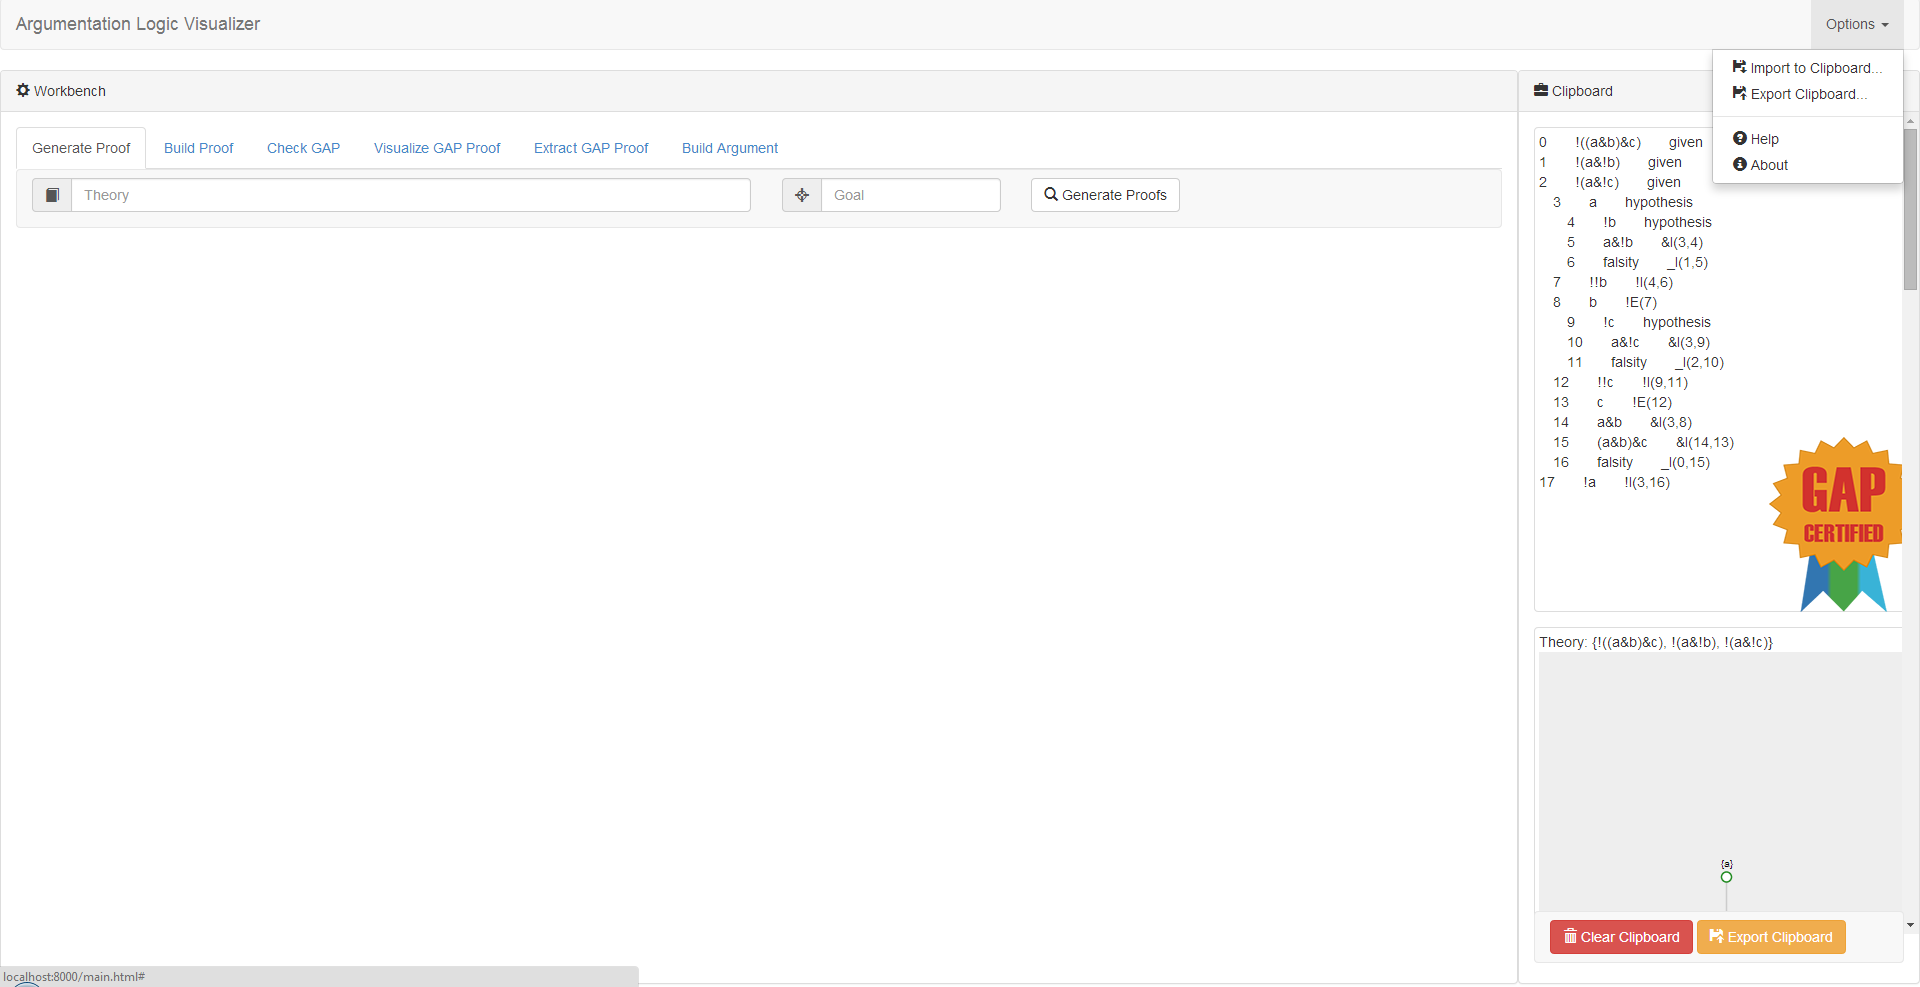
\includegraphics[scale=0.3,angle=90]{img/scr-client-all.png}}
\caption{The client GUI showing the workbench on the right, the clipboard on the left and the options on the top right corner\label{fig:scrclientall}}
\end{figure}

\subsection{Clipboard}
The clipboard holds proofs and other items that need to be retained. It acts as storage but also acts as a pool of available items to use on the Workbench.

The clipboard is always visible on the right hand side of client application as shown in \autoref{fig:scrclientall}.

\subsubsection{Thumbnails}
Each item is rendered in its own thumbnail, and can be dragged to its appropriate placeholder on the "workbench" (explained later) or on the "Clear Clipboard" or "Export Clipboard" buttons described later. \autoref{fig:scrclientthumb} shows three different items, each rendered in a thumbnail: a proof, another proof that follows the Genuine Absurdity Property, and finally, an argument.

\begin{figure}[htp]
\centerline{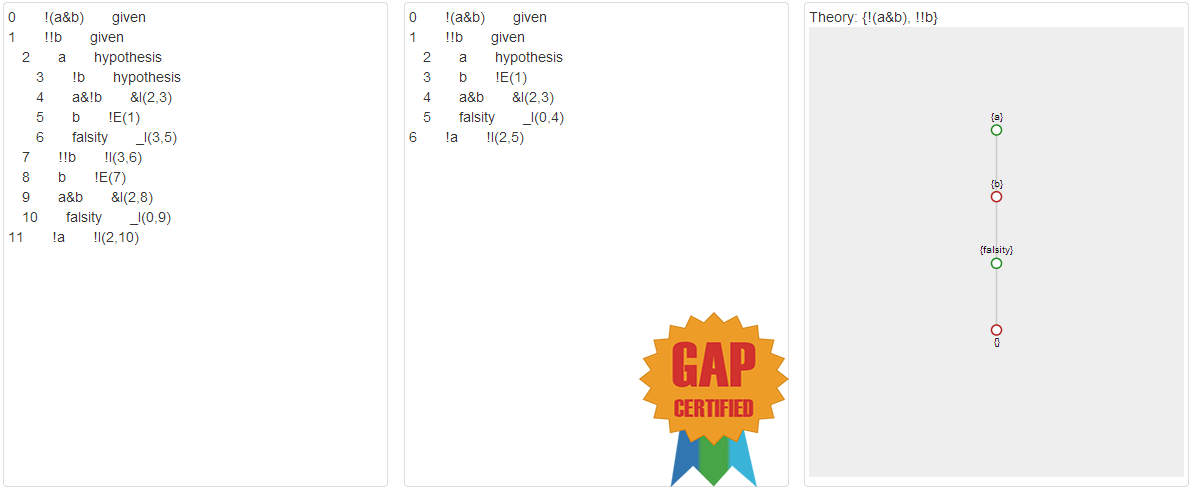
\includegraphics[scale=0.4]{img/scr-client-thumb.png}}
\caption{Three thumbnails, from left to right: a proof, a verified Genuine Absurdity Property proof, and an argument\label{fig:scrclientthumb}}
\end{figure}

\subsubsection{Persistent Storage}
The application makes use of HTML 5's \href{http://en.wikipedia.org/wiki/Web\_storage}{web storage}\footnote{http://en.wikipedia.org/wiki/Web\_storage} feature in order to provide persistent storage for the items in the clipboard. The content of the clipboard remains intact even if the webpage is closed or reloaded. However, this storage may be deleted if the browser clears its data, so it should not be heavily relied upon. There is an export clipboard feature that can export the items stored in the clipboard.

The web storage keeps the clipboard in sync with itself. Whenever an item is added or deleted, or when the clipboard is cleared using the "Clear Clipboard" button, the web storage is updated accordingly. The data is automatically loaded back into the clipboard when the page is refreshed.

\subsubsection{Managing the Clipboard}
The clipboard allows the deletion of its contents, either in its entirety or one by one. Clicking the "Clear Clipboard" button will delete all the contents of the Clipboard, but after a warning pop-up appears (as shown by \autoref{fig:scrclientcleaboard}). Dropping an item from the clipboard onto this button will delete the item from the clipboard. There is no warning pop-up for dragging a single item onto this button and that item is deleted immediately.

Clicking on the "Export Clipboard" button will export the entire clipboard. A thumbnail can also be dragged and dropped onto the "Export Clipboard" button. This will open a new window with the exported item inside. The import/export facility is discussed in \autoref{subsec:uioptions}.

\begin{figure}[htp]
\centerline{
\includegraphics[scale=0.6]{img/scr-client-clearclipboard.png}}
\caption{A notification pops up when the user clicks on the "Clear Clipboard" button that asks for confirmation\label{fig:scrclientcleaboard}}
\end{figure}

\subsection{Workbench}
The Workbench is where the different actions happen. The different tasks that can be performed have been split into tabs that all fall under the workbench. Some of these tasks require the user to input pre-made proofs or arguments from the Clipboard, or to input logic sentences or natural deduction steps. The syntax used for logic sentences and natural deduction is explained in \autoref{subsec:clyntax}. The workbench is always located on the left hand side of the screen, and occupies most of the real estate of the client screen as shown in \autoref{fig:scrclientall}.

\subsubsection{Generate Proof Tab}
The purpose of this tab is to let the user enter a theory and a goal and use the theorem prover from \autoref{chap:prover} to return all the proofs that prove the goal set by the user.

The user enters a comma-separated list of formulas in the theory input box, and a single formula in the goal input box, and clicks on the "Generate Proofs" button in order to send the data to the server. If the parsed input is incorrect, the input field with the incorrect input will be highlighted so that the user can amend their input. This is shown in \autoref{fig:scrclientgenprooffail}. As soon as all the proofs are generated and sent back, the space below the text fields and button will display the proofs as shown in \autoref{fig:scrclientgenproof}. The user can then drag the preferred proofs onto the clipboard to save them.

\begin{figure}[htp]
\centerline{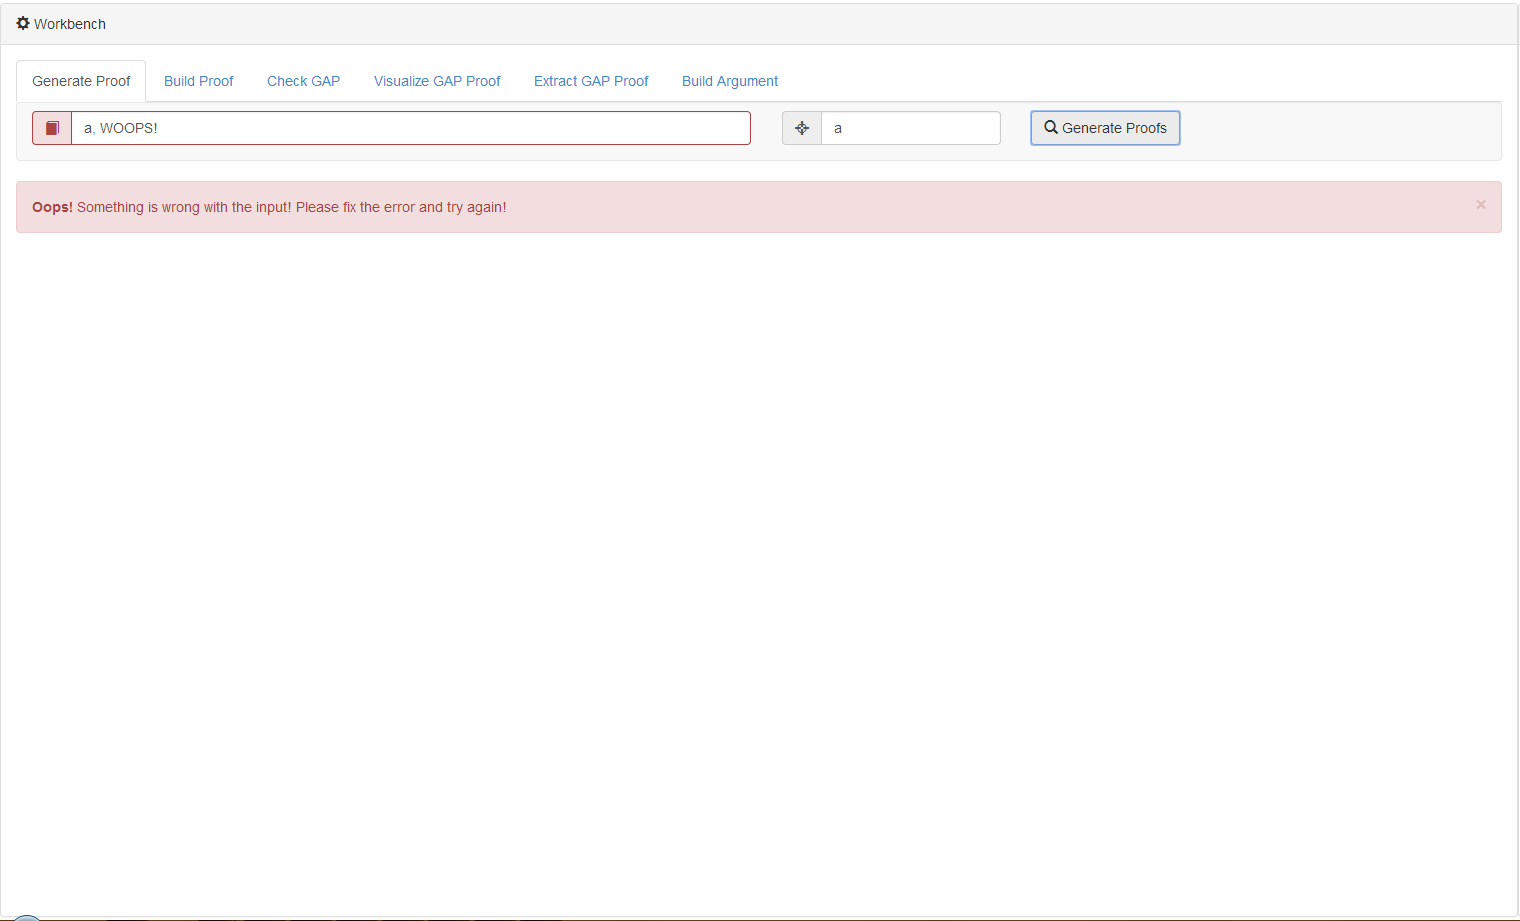
\includegraphics[scale=0.3]{img/scr-client-genprooffail.png}}
\caption{Incorrect input is highlighted so that the user can revise it\label{fig:scrclientgenprooffail}}
\end{figure}

\begin{figure}[htp]
\centerline{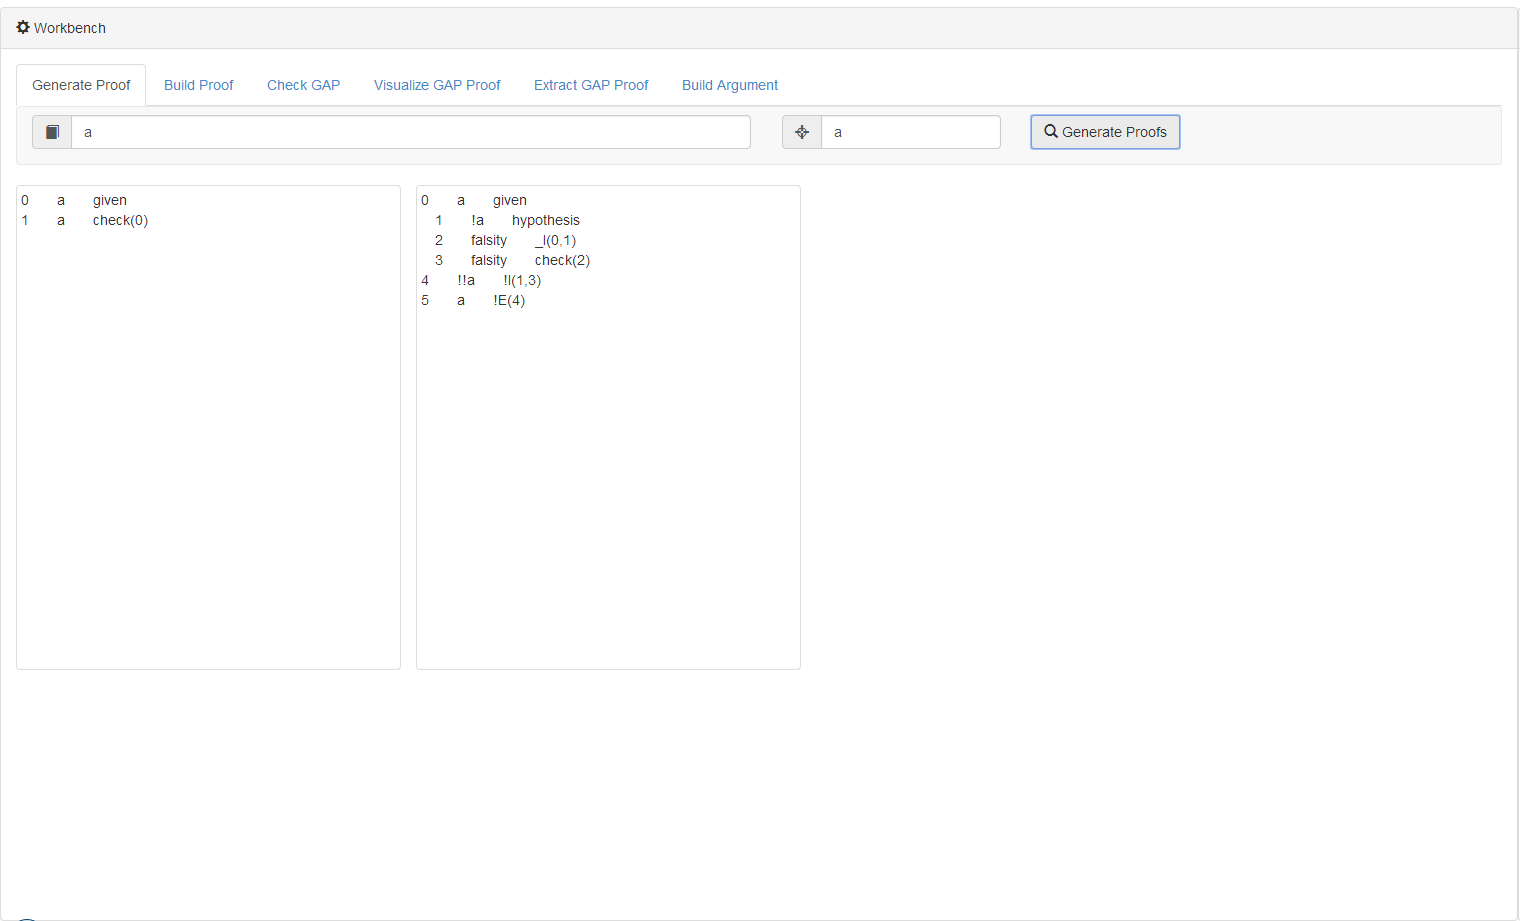
\includegraphics[scale=0.3]{img/scr-client-genproof.png}}
\caption{The theorem prover generates all the proofs that arrive to the given goal using the supplied theory\label{fig:scrclientgenproof}}
\end{figure}

\subsubsection{Build Proof Tab}
This functionality is only available in the client module. The core module does not have an equivalent function. It is described in its own separate chapter in \autoref{chap:proofbuilder}.

\subsubsection{Check GAP Tab}
This tab is used to validate proofs as following the Genuine Absurdity Property. The user can drag a proof from the clipboard that has not already been verified onto the thumbnail placeholder under that tab. The placeholder will then be filled in with the proof. The next step is to select the version of the Genuine Absurdity Property (discussed in \autoref{chap:gapcheck} and \autoref{chap:gapx}) the user would like to use. This could be either the original definition or the extended definition. This is shown by \autoref{fig:scrclientcheckgapsem}. 

Finally, the user can click on the "Check GAP" button in order to check whether the proof does indeed follow the Genuine Absurdity Property by querying the server. If the proof follows the property then this is shown by a small ribbon at the bottom right edge of the thumbnail containing the proof under examination as shown in \autoref{fig:scrclientcheckgap}. The user can then drag the Genuine Absurdity Property-verified proof onto the clipboard.

\begin{figure}[htp]
\centerline{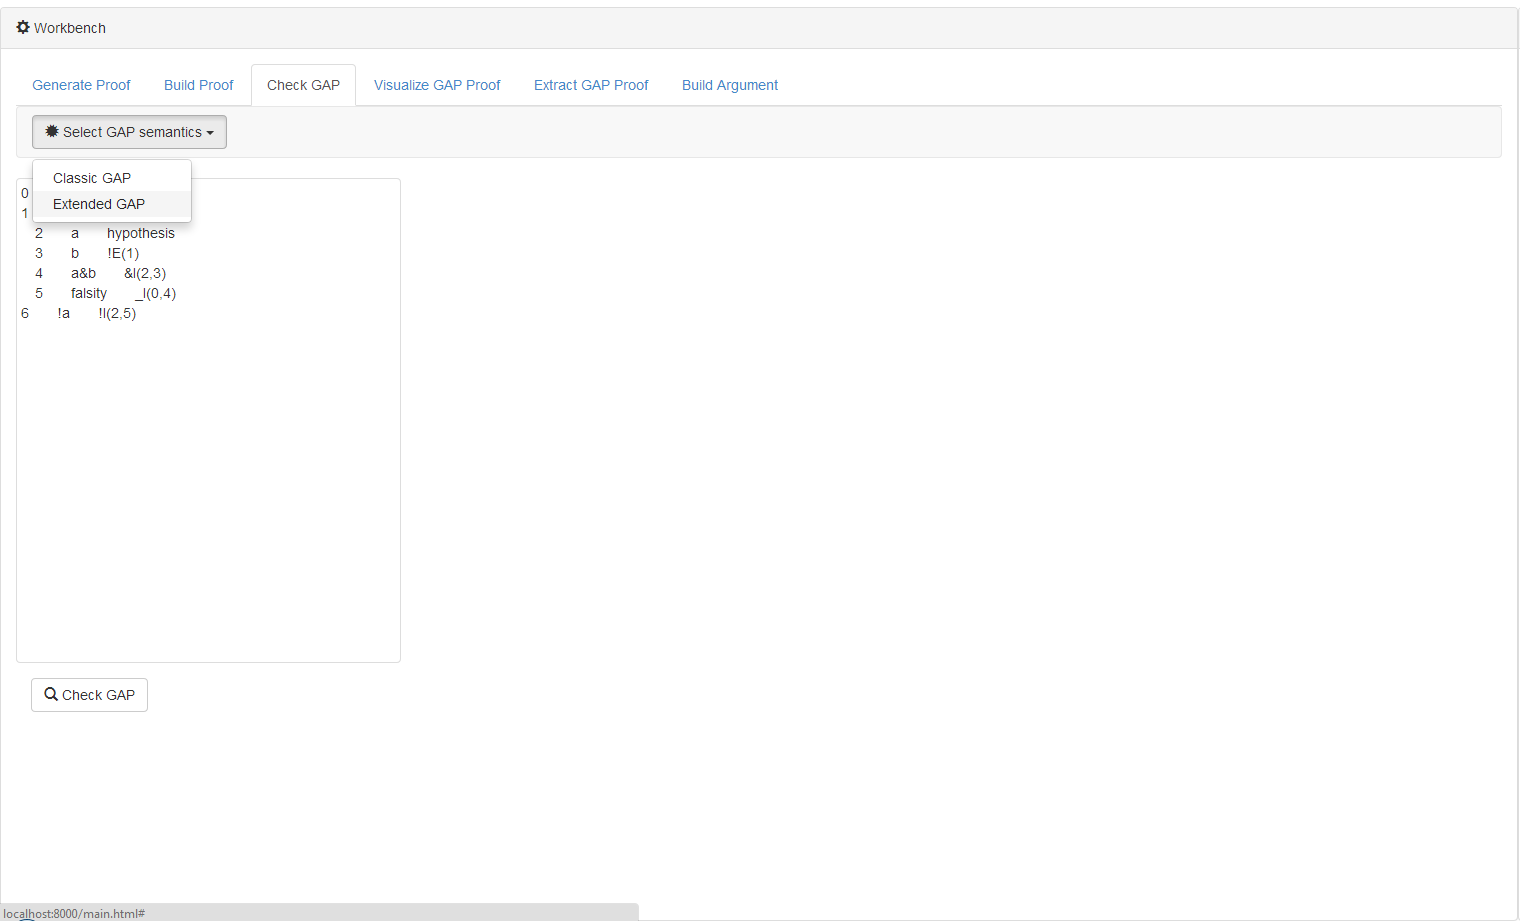
\includegraphics[scale=0.3]{img/scr-client-checkgapsem.png}}
\caption{The user can drop an unverified proof onto the placeholder and select between the original and extended definitions for the Genuine Absurdity Property\label{fig:scrclientcheckgapsem}}
\end{figure}

\begin{figure}[htp]
\centerline{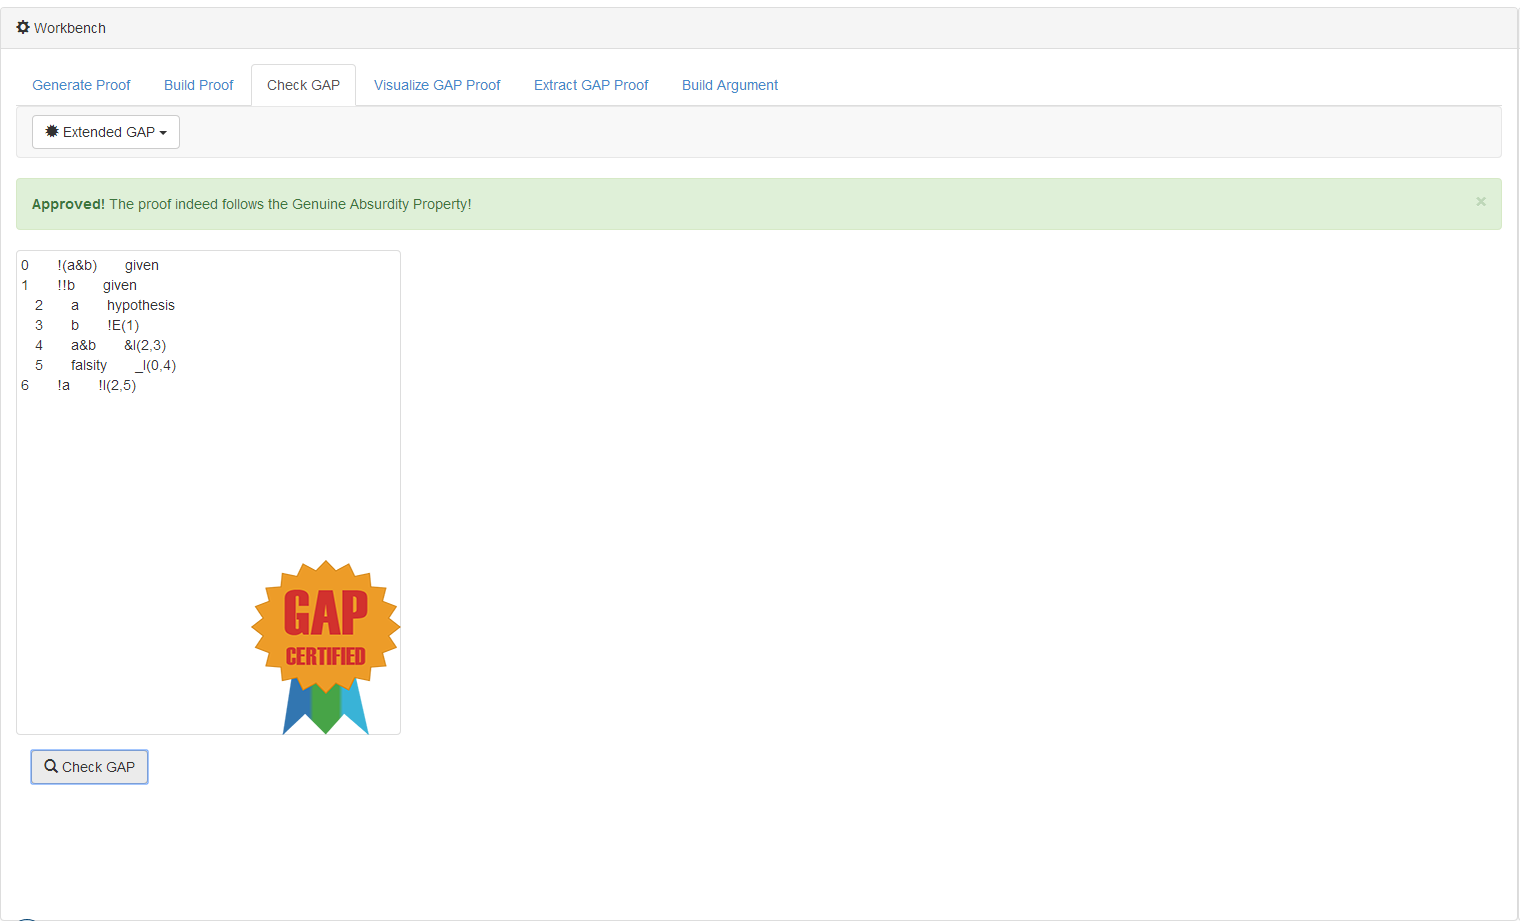
\includegraphics[scale=0.3]{img/scr-client-checkgap.png}}
\caption{If the proof follows the Genuine Absurdity Property it is indicated using a ribbon\label{fig:scrclientcheckgap}}
\end{figure}

\subsubsection{Visualize GAP Tab}
This tab allows for Genuine Absurdity Property-compliant proofs to be visualized using the algorithm devised in \autoref{chap:viz}. This tab holds two placeholders. The user can drag a compliant proof from the clipboard onto the left placeholder and click on the "Visualize GAP Proof" button. The proof will then be visualized into an argument and placed onto the right placeholder so that they can be viewed side-by-side. Finally the user can drag the visualization onto the clipboard in order to save it. A proof and its corresponding argument are shown side-by-side in \autoref{fig:scrclientproofviz}.

\begin{figure}[htp]
\centerline{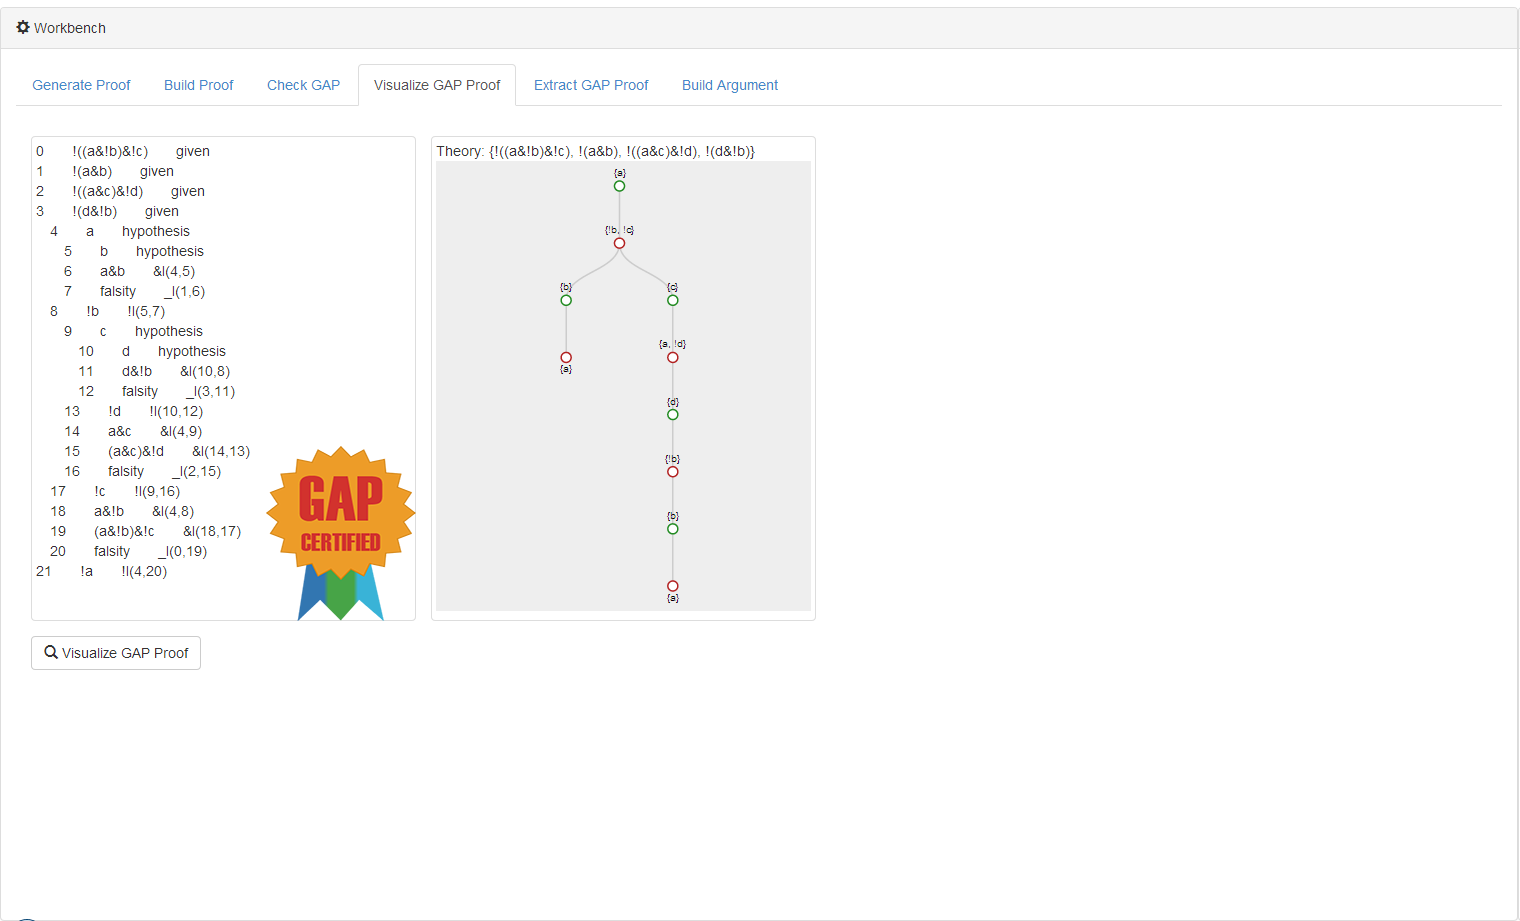
\includegraphics[scale=0.3]{img/scr-client-proofviz.png}}
\caption{The Visualize GAP tab with a given verified proof and its corresponding argument\label{fig:scrclientproofviz}}
\end{figure}

\subsubsection{Extract Proof Tab}
This tab is used to transform an argument back to a proof using the extraction algorithm in \autoref{chap:extractor}. This tab works much in the same way as the previous tab but with the input and output reversed. The user can drag a visualization (argument) onto the box on the left from the clipboard, and click on the "Extract GAP Proof" button. A proof will then be extracted from the argument and placed onto the right placeholder so that they can be viewed side-by-side. Finally the user can drag the extracted proof onto the clipboard in order to save it. An argument and its corresponding proof can be seen together in \autoref{fig:scrclientargviz}.

\begin{figure}[htp]
\centerline{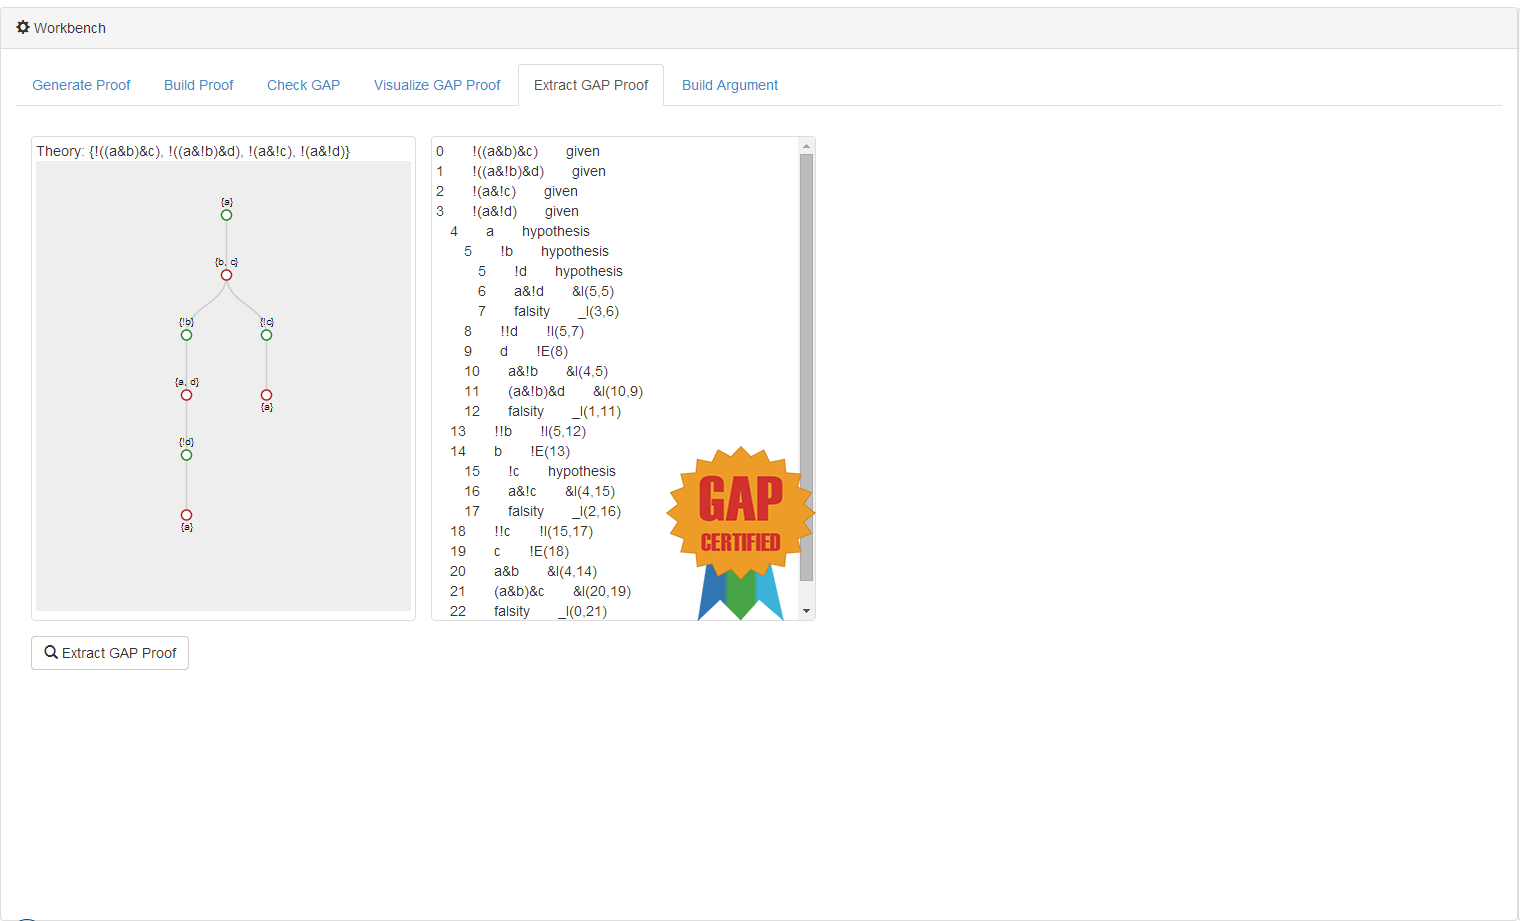
\includegraphics[scale=0.3]{img/scr-client-argviz.png}}
\caption{The Extract GAP Proof tab with a given argument and its corresponding verified proof\label{fig:scrclientargviz}}
\end{figure}

\subsubsection{Build Argument Tab}
This functionality is only available in the client module. The core module does not have an equivalent function. It is described in its own separate chapter in \autoref{chap:argbuilder}.

\subsection{Options}
\label{subsec:uioptions}
Options can be accessed via the top-right dropdown menu above the clipboard as shown in \autoref{fig:scrclientall}. A summary of the options is given below:

\begin{tabular}[htp]{|l|l|}
\hline
Option & Description\\
\hline
Import to Clipboard & Used to import exported items back to the Clipboard \\
\hline
Export Clipboard & Exports the current items in the Cliboard\\
\hline
Help & Opens a help page in a new tab with the user manual\\
\hline
About & Displays a pop-up with acknowledgments\\
\hline
\end{tabular}

The importing-exporting facility is described below.

\subsubsection{Exporting from the Clipboard}
The data stored in the clipboard can be exported as strings of JSON text and can be saved/distributed/etc. Clicking on the "Export Clipboard" drop-down menu (or button on the clipboard) will export the entire contents of the clipboard. The data will be opened in a new window. If only one of the items on the clipboard needs to be exported, simply drag that item onto the clipboard's "Export Clipboard" button. Note that exporting items from the clipboard does not delete them from it.

\subsubsection{Importing to the Clipboard}
The text exported by the "Export Clipboard" drop-down menu or button can be imported back into the clipboard by clicking on the "Import to Clipboard" drop-down menu. A pop-up appears with an input field that allows to paste the JSON text in (see \autoref{fig:scrclientimport}). Clicking on the "Import to Clipboard" button will validate the pasted text and if the validation succeeds, the parsed data will be added back to the clipboard. If the validation fails however, the input field will turn red, giving the user the chance to fix the errors and try again.

\begin{figure}[htp]
\centerline{
\includegraphics[scale=0.6]{img/scr-client-import.png}}
\caption{A pop-up shows when the user clicks the "Import to Clipboard" button on the options dropdown menu\label{fig:scrclientimport}}
\end{figure}

\subsection{Logic Syntax and Natural Deduction in Client Module}
\label{subsec:clyntax}
This section introduces the syntax used for propositional logic by the client, and how a natural deduction proof is represented.
\subsubsection{Symbols for Propositional Logic}
In order to make the application appear the same on different devices with different character encoding abilities ASCII characters were used to represent logical connectives. \autoref{tab:clyntax} summarizes the different symbols used and what they represent.

\begin{figure}[htp]
\begin{center}
\begin{tabular}{|l|l|}
\hline
Symbol & Meaning\\
\hline
$!$ & Negation\\
\hline
$\&$ & Conjunction\\
\hline
$|$ & Disjunction\\
\hline
$->$ & Implication\\
\hline
$\_$ & Falsity (Contradiction)\\
\hline
$()$ & Precedence (Grouping)\\
\hline
\end{tabular}
\end{center}
\caption{The logical symbols used by the client application \label{tab:clyntax}}
\end{figure}

The same symbols are used by the parser as well.

\subsubsection{Entering Propositional Formulas}
Single propositional formulas can be entered by typing in the formula using the symbols shown above. This is usually required when entering a goal to be proven. A list of propositional formulas is a comma-separated list of formulas. Space characters are ignored. Lists of formulas are usually required when specifying the theory (which might consist of more than just one formula).

\subsubsection{Natural Deduction Format}
With the exception of the symbols used to indicate logic constructs, natural deduction is represented in the same way as it is represented in this paper. In \autoref{sec:nd} a summary of the rules used by the client as well as an example on how the natural deduction proofs look like are provided. The boxes (sub-derivations) are represented with an indentation rather than an actual drawn box. The greater the indentation, the deeper the sub-derivation is.

\section{Alternatives}
\label{sec:clientalt}
There is a wide variety of alternate implementations for the user interface. Among them exist the following:
\begin{itemize}
\item
\href{http://en.wikipedia.org/wiki/Swing\_(Java)}{Java Swing}\footnote{http://en.wikipedia.org/wiki/Swing\_(Java)}
\item
\href{http://www.swi-prolog.org/packages/xpce/}{Prolog XPCE}\footnote{http://www.swi-prolog.org/packages/xpce/}
\item
\href{http://www.gtk.org/}{GTK+}\footnote{http://www.gtk.org/}, \href{https://qt-project.org/}{QT}\footnote{https://qt-project.org/}, and other similar application frameworks or widget toolkits
\end{itemize}

Swing is a Java widget toolkit. It can be used to create platform-independent user interfaces written in Java, much in the same way as HTML, CSS and JavaScript can be used to make cross-platform applications. Java tends to be quite verbose however, leading to more complicated code sometimes. The major difference lies in the fact that Swing is used in Java applications, whereas JavaScript is used in web applications. Swing could have been used to create an interface that is packaged together with the server, merging the two roles in one application (ie there would be no physical separation between the client and server), if a Prolog binding library were used (like JPL). This would make the use of a web browser unnecessary.

Prolog XPCE is a SWI-Prolog library for creating graphical user interfaces. This would be the most preferable option since the interface could have imported the core module directly, rendering the server obsolete. Prolog code tends to be very concise, unlike graphical user interface code in general. However, the look and feel of the interfaces produced by XPCE is a bit dated, and more modern alternatives are out there that could offer a better overall experience.

GTK+, Qt and other similar widget toolkits have been proven by various well-known applications for their wide variety of interface elements and overall flexibility. These libraries tend to be very fast, since they are written in C or C++. This however, makes it difficult to produce bug-free interfaces because of their complexity and code size. There have been efforts to create bindings to other high-level programming languages such as Python (\href{http://www.riverbankcomputing.com/software/pyqt/intro}{PyQt}\footnote{http://www.riverbankcomputing.com/software/pyqt/intro} and \href{http://www.pygtk.org/}{PyGTK}\footnote{http://www.pygtk.org/}) that drastically simplify the making of graphical user interfaces with the aforementioned libraries.

The major advantage of building a web application, and the major disadvantage of desktop applications, is deployment. For web applications, updates do not need to be pushed down to the client, and the client itself does not need to seek updates from a server. That is because a web application is served by the server directly, and so application updates can be hot-swapped whenever they become available. A simple page refresh is all that is required. Thus the major advantage of choosing HTML, JavaScript and CSS is that it allows for the option of hosting the project on a public webserver, and allowing the client to be sent to the user's web browser as a web application. This is not possible with the aforementioned alternatives.

In addition, web development has become very fast, with different toolkits and libraries available that speed up development and significantly increase productivity. Web applications can now run at very high speeds due to sophisticated JavaScript engines incorporated by web browsers. In this respect, the current solution does not lack in terms of performance, productivity or appearance, and has the distinct advantage of quick and easy distribution.

\chapter{Proof Builder}
\label{chap:proofbuilder}
Experience from repeated usage of the theorem prover in order to generate proofs has shown that sometimes the amount of proofs generated using the theorem prover directly can be overwhelming. Most of the time, a particular proof was required for further study, and going through the generated results was found tedious. Thus a need for a proof builder arose, so that when a particular proof is required, it can be input directly with the help of the proof builder.

\section{Motivation for Client Side Implementation}
The proof builder is completely client side. There are several reasons for this decision. 

Firstly, since this is an aided construction, visual feedback should be frequent and immediate. Requesting validation from the server would be both wasteful in terms of resources and possibly time-consuming as the builder would stall until the response comes back from the server. 

Hence by building this feature client side, unnecessary back-and-forth communication is avoided. 

Since the proof builder is completely contained in the client, it can be easily integrated into the GUI for a seamless experience that can be used offline as well. 

Since this feature involves a gradual construction of a proof with intermediate user input, keeping the current state is essential. Since the proof builder is client side, it does not communicate with the server and therefore the server does not need to hold any session information and can indeed be completely stateless.

\section{Features}
The proof builder features a very simple, easy to use interface. The interface is made of two input fields where the user can input the theory and goal of the proof, a button that signifies the start of a new proof, a placeholder for rendering the current state of the proof, and finally, one more input box for entering commands to guide the construction of the proof.

The proof builder makes use of the client's text input parser. The parser can report incorrect input and validate the user's commands to the proof builder. For example, if the user enters the command $a\&b; \&I(5)$ (which means that a new step is to be added where the derivation is $a\wedge b$ and the reason is $\wedge$-introduction from line 5), the parser will detect that a $\wedge$-introduction rule requires two line references instead of the one provided (one for each of the two subformulas of the conjunction) and will make the command input box glow red to indicate an error.

Even if the input is syntactically correct, mistakes can still happen. Assuming correct syntactically input that passed the parser stage, the natural deduction rule checker can be used to verify the command. Line references will be checked, and the rule application will be verified as well. For example if the user enters an erroneous command $a\&b; \&I(5, 9000)$ and the current step to be added has line number 5, then this is picked up by the rule checker. The rule checker can work out if the derivation was made correctly. For example if the given input is $a\&b; \&I(5,3)$, the rule checker will see that this is supposed to be an application of the $\wedge$-introduction rule. This means that the derivation should be a conjunction of two sub-formulas. Those subformulas ($a$ and $b$ in the example) should have previously been derived on the lines referenced by the command (lines 5 and 3 in the example). If any error occurs, the command input box glows red to signal incorrect input. The effect of this is that proofs generated by the proof builder are sound.

As mentioned above, feedback is given immediately after the user enters a command. Even if the feedback is not very specific, it is adequate for the user to understand what went wrong with just a brief inspection of their input. Since feedback is available immediately after each command entered, and because no progress can be made if the command is not valid, the user can easily identify the mistake.

\section{Usage}
The user starts by navigating to the "Build Proof" tab of the Workbench. There, two input boxes can be found. In the first one, a comma-separated list of formulas can be entered for the theory. In the second input field, a single formula may be entered for the goal of the proof. This is used by the proof builder to identify when the proof is complete. The user clicks on the "Build Proof" button and the proof construction begins if the theory and goal parse correctly. If not, then whichever field contains erroneous input is highlighted. If the parsing succeeds then the command input field is enabled and is ready for use. The theory is already filled in with "given" being the reasons of the steps of the proof. \autoref{fig:scrclientproofbuilder} shows this state.

\begin{figure}[htp]
\centerline{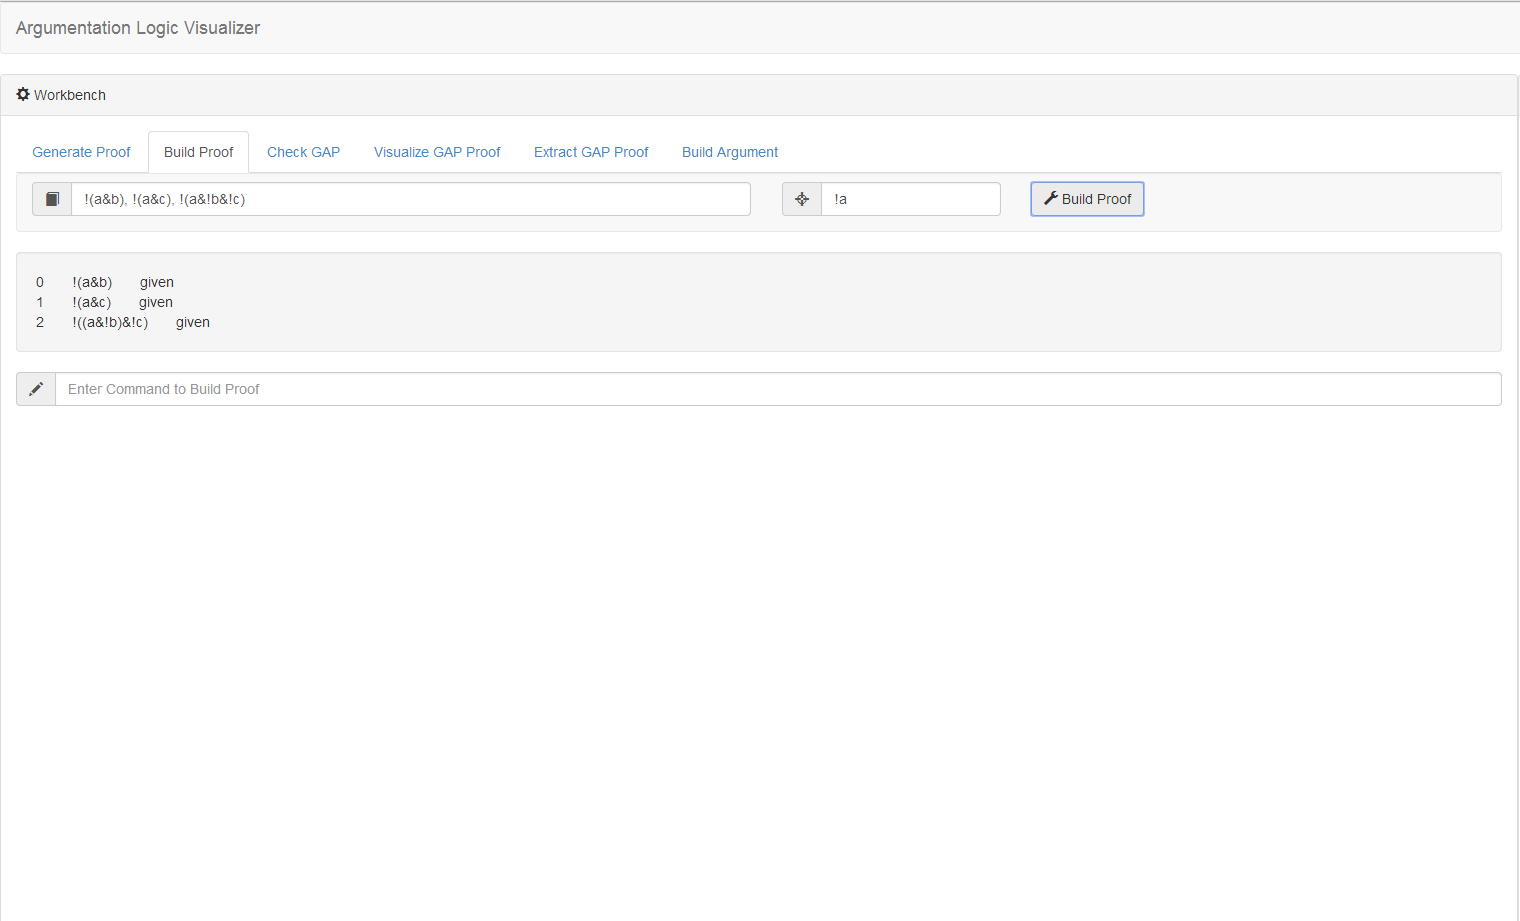
\includegraphics[scale=0.3]{img/scr-client-proofbuilder.png}}
\caption{The proof builder already fills in the theory as steps for the proof that the user is about to build\label{fig:scrclientproofbuilder}}
\end{figure}

The user can type commands in the command input field below the rendered proof under construction and enter them by pressing the Enter key. If the command is accepted, it is executed. Otherwise, the command input field glows red to indicate an error. This is shown in \autoref{fig:scrclientproofbuilderr}. There are three supported commands:

\begin{figure}[htp]
\centerline{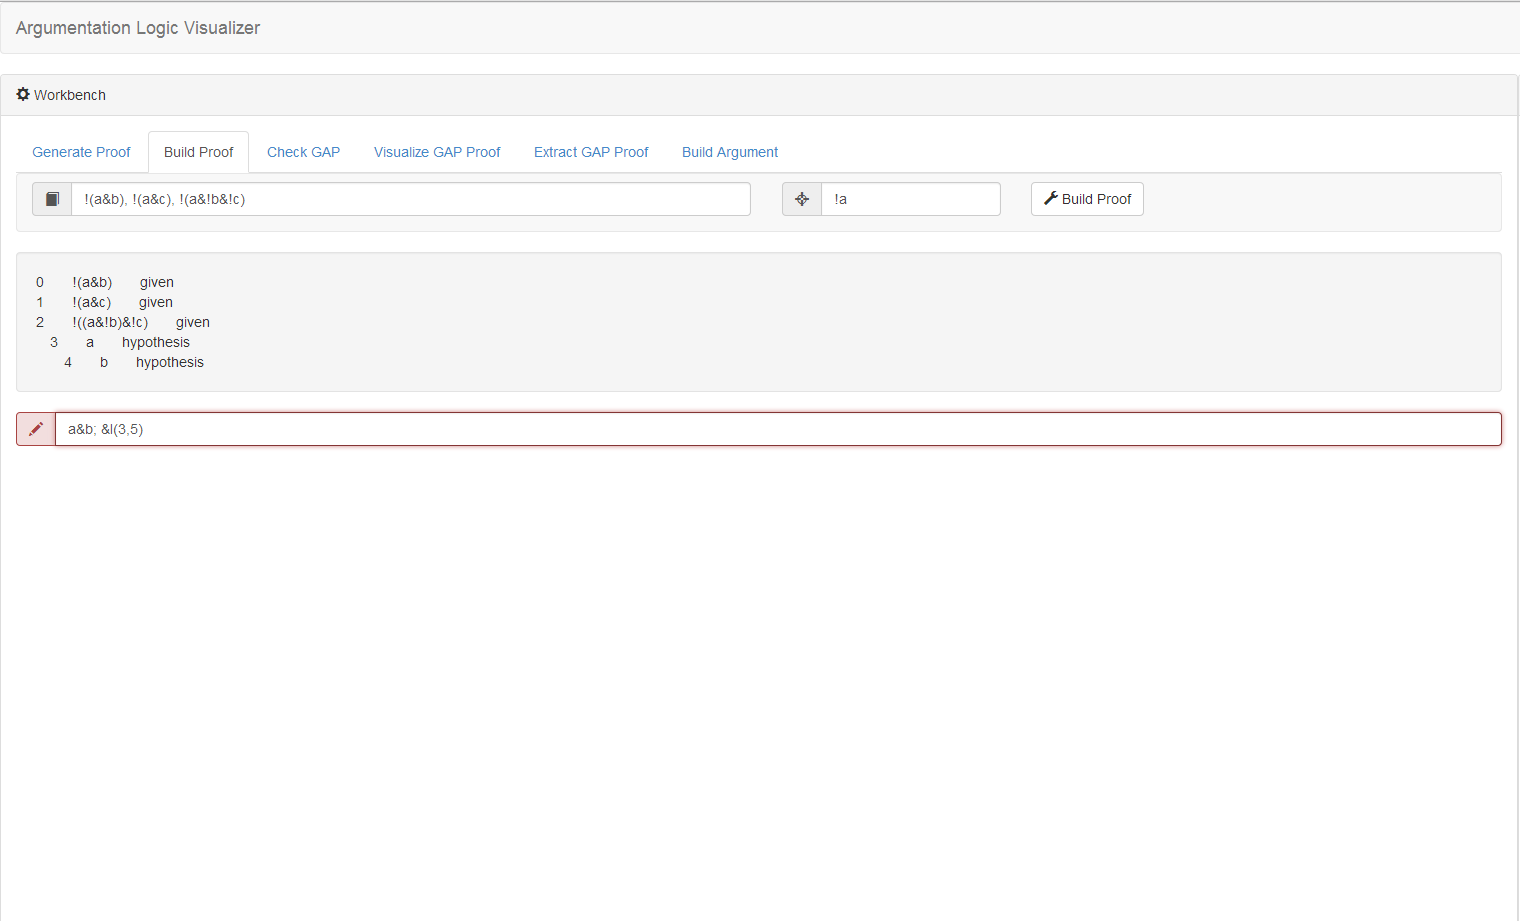
\includegraphics[scale=0.3]{img/scr-client-proofbuilderr.png}}
\caption{The proof builder indicates an error when the user input is incorrect\label{fig:scrclientproofbuilderr}}
\end{figure}

\begin{itemize}
\item
New step: adds a new line at the end of the proof under construction
\item
Delete last step: deletes the last line of the proof
\item
Delete last n steps: deletes the last n steps of the proof
\end{itemize}

The first command is of the format $[formula]; [reason]$, where $[formula]$ is any valid formula and $[reason]$ is any of the supported reasons listed in \autoref{fig:ndrulesproofbuilder}. These can be compared to \autoref{subsec:logicrules}. If the step command is a new hypothesis, a box is automatically opened. Boxes are shown by an indentation of the lines of the proof proportional to the level of nesting. If the step command describes a $\neg I$ step, then the current box is closed and the command is appended one level up.

\begin{figure}
\begin{tabular}[htp]{|l|l|l|}
\hline
Rule Format & Rule Name & Description\\
\hline
$\&I(\#,\#)$ & $\wedge I$ & Conjunction of the formulas indicated by the two referenced\\ 
&& lines\\
$\&E(\#)$ & $\wedge E$ & The left/right hand side of a conjunction indicated by the\\
&& referenced line\\
$->I(\#,\#)$ & $\rightarrow I$ & Implication of two formulas at the start or end of preceding\\
&& box indicated by the referenced lines\\
$->E(\#,\#)$ & $\rightarrow E$ & Right hand side of implication derived by an implication \\
&& and its left hand side indicated by the referenced lines\\
$\_I(\#,\#)$ & $\bot I$ & Contradiction introduced by a formula and its negation as \\
&& indicated by the referenced lines\\
$\_E(\#)$ & $\bot E$ & Any formula derived from a contradiction indicated by the \\
&& referenced line\\
$!I(\#,\#)$ & $\neg I$ & The negation of a hypothesis and a subsequent contradiction \\
&& in a box as indicated by the referenced lines\\
$!E(\#)$ & $\neg E$ & The derivation of a formula by removing a double-negation \\
&& from a formula indicated by the referenced line\\
$hypothesis$ & $hypothesis$ & A hypothesis placed at the beginning of a box\\
$check(\#)$ & $reiteration$ & Restating a previously derived formula\\
\hline
\end{tabular}
\caption{Supported natural deduction rules for the proof builder. A \# represents a line number\label{fig:ndrulesproofbuilder}}
\end{figure}

The second command is of the format $--$. This deletes the last line of the proof. If that line was a $\neg I$ or $\rightarrow I$ rule then the preceding box is now re-opened and can be closed by issuing another $\neg I$ or $\rightarrow I$ step command.

The last command is of the format $-[number]$, where $[number]$ is any non-negative number. The last $n$ steps are deleted where $n$ is the number specified. This command works by repeating the second command $n$ times so the effects are essentially the same.

The user can enter commands to fill in the proof. When the last step in at the top level (not inside a box) and it matched the goal entered at the very start, then the proof is complete and the command input box is disabled. The rendered proof now becomes draggable and the user can subsequently drag the proof onto the clipboard to save it. Underneath the user interface, the proof has the same exact representation as a proof generated by the theorem prover, and can thus be used to check whether it follows the Genuine Absurdity Property, be visualized (if it does indeed follow the property) and so on.

\chapter{Argument Builder}
\label{chap:argbuilder}
In order to complement the proof builder (\autoref{chap:proofbuilder}) an argument builder was created so that specific arguments can be drawn directly, without first having to create the corresponding proof. 

Much in the same way as the proof builder works, the argument builder provides immediate feedback to the user during the construction of the argument. Unlike the proof builder however, the argument builder is not completely client side. This is due to the fact that the theorem prover needs to be used in order to justify attacks claimed by the user.

The data sent to the server is minimal however, since the only communication between the client and the server when using this builder is a query about whether the supplied theory and given attack claim causes a contradiction with the defense, and does not cause a contradiction without it. The latter is used to check that the actual attack makes sense in that it attacks the defense, and not the theory itself.

Even though the argument builder makes use of the server, all of the state (the theory and the argument under construction) is held locally. This allows the server once more to be stateless. This means that the server does not need to remember any sessions and connections from the clients, greatly simplifying the overall architecture and future maintenance of the project.

\section{Features}
The argument builder makes use of a simple user interface, using elements from other parts of the overall interface. It consists of two input fields for the theory and the first argument, a thumbnail which shows the argument under construction and an attack input field, where the user can specify their attacks.

The argument builder benefits from the same parser that the proof builder and the rest of the client use, which can check that the theory, starting argument and subsequent attacks are syntactically correct.

At the same time, the argument builder uses a $NACC$-semantics checker, which checks the valid attacks made by the user and automatically ends the attack-defense chain when the attacks form terminal nodes (leaves).

The argument builder features automatic generation of defenses, and termination of the construction of the argument if all branches lead to terminal attacks.

\section{Usage}
The construction of an argument involves a mini-game where the user gives the argument builder the theory and initial argument (the first "defense", or the first argument of the "proponent"). Then it is the job of the user to attack the computer, specifying attack claims. Claims that form good attacks, are accepted and added to the tree. The "proponent" (the computer) then automatically generates the defenses, since they are very well predictable and specified (\autoref{subsec:alfdef2}, \nameref{subsec:alfdef2}). When all branches have been closed off (blocked by a terminal attack), the mini-game ends and the user can save the constructed argument.

The user starts off by entering the theory and argument that should be defended by the computer. The user then clicks the Build Argument button in order to begin the construction of the argument. If an error in the input is detected by the parser, the offending input box is highlighted. Upon the beginning of the construction, the first argument of the proponent is visualized. The attack claim input field is then enabled and the program awaits the user's attack. This state is shown in \autoref{fig:scrclientargbuilder}. The user can make an attack claim by first specifying what the attack is going to be. In order to do that, the user enters the attack in the attack input box and presses the Enter key on the keyboard. If the attack makes sense (does not contradict the theory itself), then it is accepted, otherwise the input field glows red to indicate a bad attack. This is similar to entering an incorrect command in the command input field of the proof builder.

\begin{figure}[htp]
\centerline{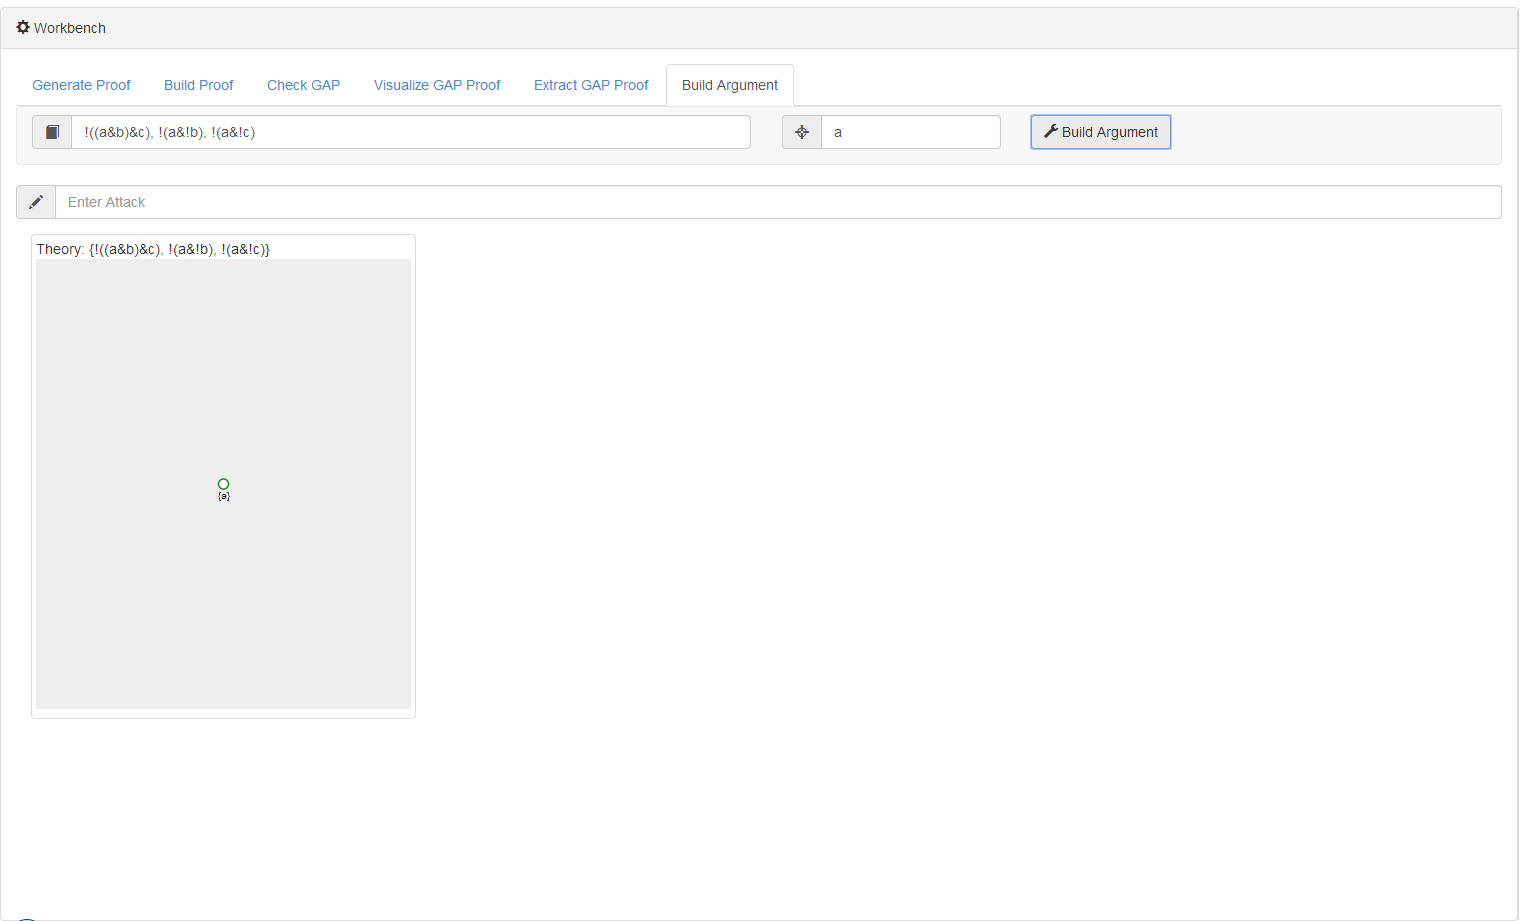
\includegraphics[scale=0.3]{img/scr-client-argbuilder.png}}
\caption{The argument builder draws the initial argument and enables the attack input field awaiting for the user's command\label{fig:scrclientargbuilder}}
\end{figure}

Green nodes represent defenses, and these are generated by the computer. Red nodes indicate attacks, and these are added by the user. If the attack is accepted, then a blue node appears on the bottom left corner of the visualized argument under construction to indicate an attack claim. This state is shown in \autoref{fig:scrclientargttack}. The user can now drag the attack claim (blue node) onto eligible nodes in the argument tree. Eligible nodes are leaf defenses. As soon as the user starts dragging the blue node, all eligible nodes will be indicated by a faint red drop zone, where the user can drop the blue node. A bright red temporary link will also link the attack claim and defense if the attack claim is hovering over its drop zone. This is shown by \autoref{fig:scrclientfinishhim}. The user can let go of the blue node to issue the attack. The attack is checked that it reaches a contradiction when combined with the defense it is attacking. If that is the case, the tree is redrawn and the attack claim is "set in stone" as it is drawn underneath the defense as a red node.

\begin{figure}[htp]
\centerline{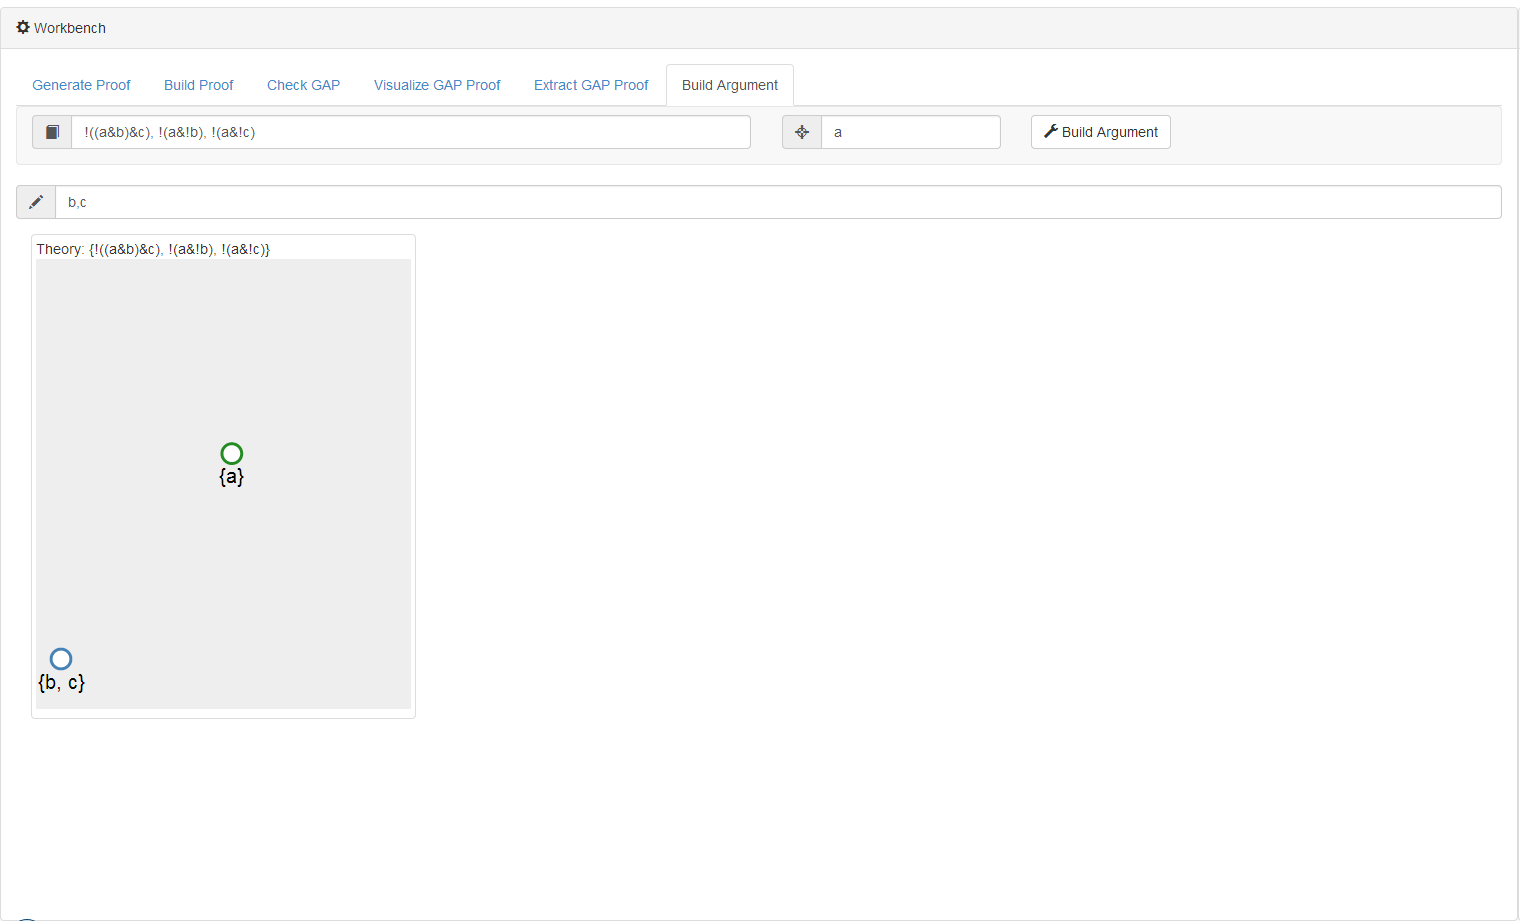
\includegraphics[scale=0.3]{img/scr-client-argttack.png}}
\caption{The argument builder draws the initial argument and enables the attack input field awaiting for the user's command\label{fig:scrclientargttack}}
\end{figure}

\begin{figure}[htp]
\centerline{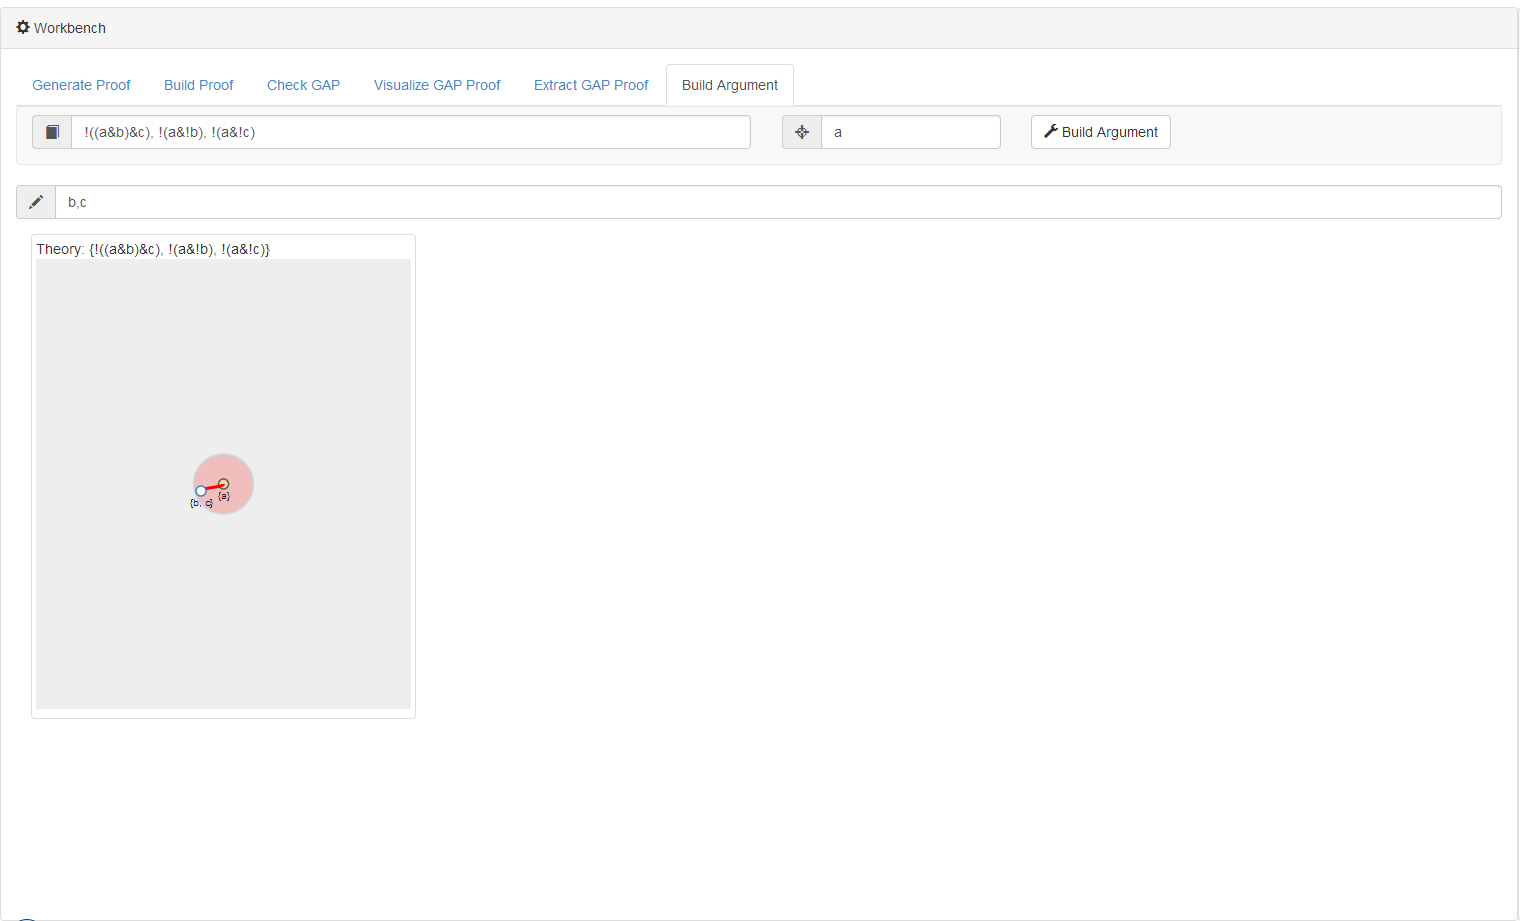
\includegraphics[scale=0.3]{img/scr-client-finishhim.png}}
\caption{The user is about to attack the computer's argument; a red link shows the node the attack will be against if the user drops the attack node\label{fig:scrclientfinishhim}}
\end{figure}

\begin{figure}[htp]
\centerline{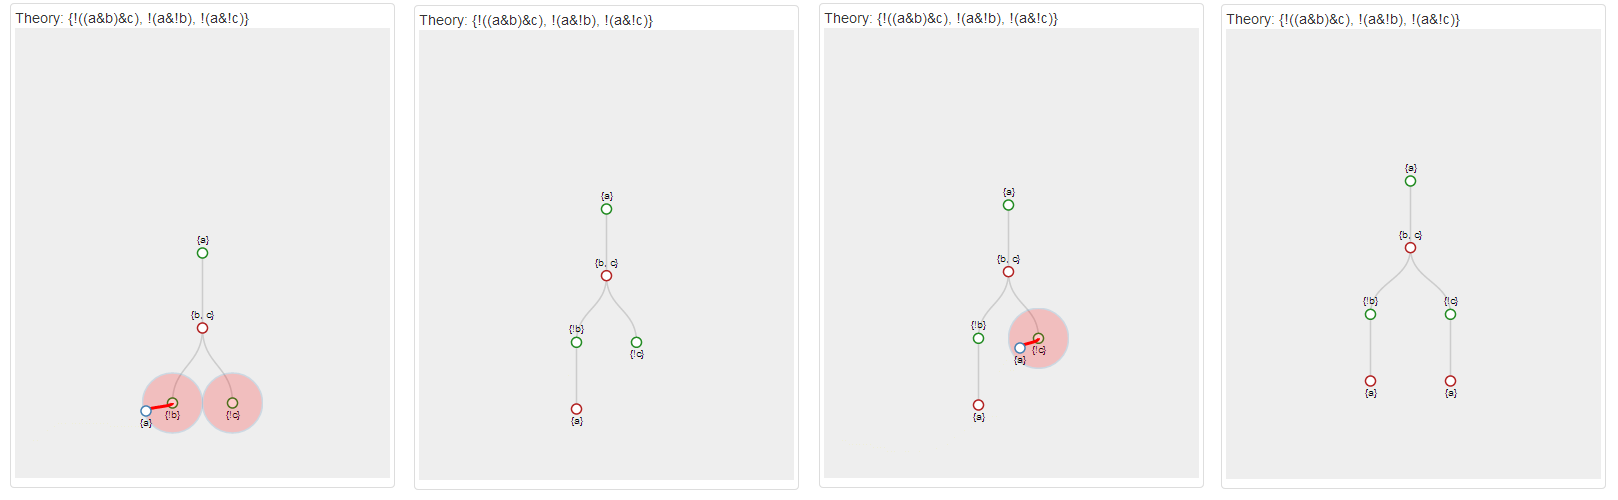
\includegraphics[scale=0.3]{img/scr-client-fatality.png}}
\caption{The user gives a terminal attack on the left branch, leaving only the right branch open; after a terminal attack on the right branch, the argument is complete\label{fig:scrclientfatality}}
\end{figure}

When the user makes a successful attack, the computer checks if the attack is a subset of the parent defenses, according to the $NACC$ semantics of Argumentation Logic (\autoref{subsec:nacc}). If it does, it is considered a terminal attack. This means that no defenses are generated to defend against that attack and hence that branch of the tree is effectively closed off (\autoref{fig:scrclientfatality}). If the attack is not a terminal attack, then defenses are generated according to the $NACC$ semantics once more. The defenses are predictable, since the definition of a defense is to take the opposite stance of a component of the attack (\autoref{subsec:alfdef2}).

The mini-game ends when all branches are closed off and no unattacked defenses remain. The attack claim input field is then disabled and the constructed argument can be dragged to the clipboard in order to be saved. The arguments generated by the argument builder have the exact same format as those generated by the visualization algorithm (\autoref{chap:viz}) and can be used in the same way.

\section{Generating Arguments Automatically}
Originally, an argument generator that works in a similar way to the theorem prover (\autoref{chap:prover}) was envisioned, which could be given a theory $T$ and a starting argument $a$ and generate all arguments proving $NACC^T(\{a\},\{ \})$. The idea was dropped as a lot of computation would be necessary to generate attacks.

In order for an attack to be generated, the argument generator would have to go through the powerset of the language and try each subset in order to test if it forms a valid attack. Defenses, given a valid attack, could be generated easily since they always take the opposite (negation) of the attack components.

Consider a small example with theory $T = \{\neg(\alpha\wedge\neg\gamma), \neg(\alpha\wedge\beta\wedge\gamma), \neg(\neg\beta\wedge\delta), \neg(\alpha\wedge\neg\beta\wedge\neg\delta)\}$. The language for this theory is $L = \{\alpha, \beta, \gamma, \delta, \neg\alpha, \neg\beta, \neg\gamma, \neg\delta\}$ and therefore the powerset of the language $\mathcal{P}$ contains 256 subsets. Almost all of these subsets will need to be processed to check whether they constitute a good attack. Some of these subsets will not constitute good attacks, for example $S_1 = \{\delta, \neg\delta\}$ (it contradicts itself) or $S_2 = \{\alpha, \neg\gamma\}$ (it contradicts the theory itself) and thus further calculations will be necessary to weed them out. This entire procedure needs to be repeated $n$ times for just one argument with $n$ number of attacks.

It is therefore only a viable solution if a good strategy can be devised that can drastically prune the search space of the possible attacks. This, consequently, remains a topic for future work.

\chapter{Evaluation}
\label{chap:eval}
Evaluation of this project cannot be based on user feedback. The implementation is not addressed at a general audience, hence statistics like number of downloads on an online store, or feedback and ratings on a particular website do not apply. At the same time, the implementation is not a piece of software that is meant to run something in a very optimized way, so statistics like frames per second, time intervals, etc are of no use either. It is difficult to evaluate the project since it is based one Argumentation Logic, that is not yet widely known. The project is mostly exploratory. Ideally the evaluation for the project should be written one or two years after its submission.

The overall project will therefore be evaluated on its correctness, stability and on its contributions, as well as on whether it fulfilled the objectives it set out to complete. This evaluation section will start its criticism by evaluating the different components, procedures and algorithms of the project and move up to its aims and objectives in general.

\section{Theorem Prover}
A critical evaluation of the theorem prover was made in \autoref{sec:tpeval} in more depth. A summary of that follows. The theorem prover strives to be sound and complete over the logic constructs it currently supports. However as with any implementation, bugs may interfere. Formal verification was deemed too taxing in terms of time, so plenty of unit tests were used instead to limit the possibility of errors. The theorem prover works, though sometimes it is slow when the search space becomes too complex. This is because the implementation does not prune any proofs because they may be valuable from an Argumentation Logic point of view. Argumentation Logic-compliant pruning (and other performance enhancements) and the introduction of disjunction are among the future improvements.

\section{Other Algorithms and Procedures}
Other algorithms and procedures include the (extended) Genuine Absurdity Property checker, the proof visualization algorithm, the proof extraction algorithm and the proof and argument builders.

Unit testing was once again employed for the Genuine Absurdity Property checkers. This is a very important procedure, so great care was taken in order for this check to be correct. Both the original definition and the extended share a great deal of similarities, and that is reflected in the conciseness and code reuse of different parts of the code.

Manual tests were plenty and thorough for all of the above procedures and algorithms. Performance was very dependent on the theorem prover. Most of the runtime of the code was spent inside the theorem prover than any of the above procedures. The runtime of these procedures was found to be negligible, suggesting very optimal solutions. The opportunity to optimize the extended version of the Genuine Absurdity Property checker was taken and the result is that siblings do not need to be rechecked whenever referenced. More details about this optimization can be found in \autoref{sec:remarx}.

Improvements include the ability to create arguments that distinguish between child derivations and sibling derivations for the visualization algorithm if that is found to be more preferable. In that way, generated arguments will contain the information that certain parts of the attacks and their defenses came from references to siblings instead of children. More information about this can be found in \autoref{sec:vizmarks}. Identifying repeating arguments and creating shorter proofs that reuse one instance of such arguments is a potential upgrade to the current proof extraction algorithm as discussed in \autoref{sec:proofmarks}.

\section{Server}
The server is a very stable and simple unit of code. It was indirectly tested extensively when testing the client (since the server was always running behind the scenes to support it). As discussed in \autoref{sec:remarklet}, it requires virtually no maintenance and a very limited amount of requirements to run.

\section{Client and User Interface}
The client strikes a balance between bells and whistles and minimalistic and intuitive interface. It is easy to use and is quite stable. No unit testing was employed in favor of manual testing, since automated GUI testing is non-trivial and quite time-consuming. In the worst case simply hitting F5 (usual shortcut for a page refresh) on the keyboard solves all problems. It has a variety of features that enhance the client's usability, listed in \autoref{sec:cleatures}.

Improvements could include database support for storing proofs and arguments. This would impose a burden on the server however, since user identification and a database setup and connection would be necessary.

\section{Overall Software Engineering Evaluation}
Despite the fact that software engineering was not the main focus of the project, great effort was made to keep the different logical modules separate, independent and extensible. The overall architecture of the project is simple and explained in \autoref{chap:solover}. The core can be used standalone, however the client provides a good wrap-around that simplifies the overall procedure of using the functionality offered by the system. Deployment is made easy because of the client-server infrastructure. Stability is not an issue, as there is a seamless interaction between the client and the server (and core). The only noticeable problem is that sometimes the server is slow to reply to the client after a request was made because the theorem prover takes longer than usual to run.

\section{Project Aims and Objectives}
One of the main objectives of the project was to explore Argumentation Logic. Argumentation Logic is a relatively new concept. 

Contributions to this concept include the extension of the Genuine Absurdity Property to work with natural deduction proofs that make use of the substitution shortcut that allows sub-derivations to refer to sibling derivations instead of re-proving what they have already proven. The extension explains how an optimization can be achieved by not re-checking sibling sub-derivations for the Genuine Absurdity Property as it does not change with respect to the content they are imported to.

Another contribution was the invention of the visualization algorithm. This algorithm or procedure, provides an exact definition as to how a proof bearing the Genuine Absurdity Property can be converted into an argument. This algorithm is also consistent with the extension of the property. This algorithm creates a mapping between attacks and defenses with respect to arguments, and contradictions and hypotheses with respect to proofs.

Along the contributions made by the project is a constructive algorithm that can turn an argument back into a proof, and this relies on the visualization algorithm definition, namely on the mapping it defines.

The final contribution of this project is the creation of a software tool that implements the aforementioned concepts and algorithms in order to provide a playground in which learners of Argumentation Logic can practice. 

The software tool also provides a proof builder and an argument builder (for Argumentation Logic), and so at a lesser degree, it can be used to learn about propositional logic and maybe argumentation.

Unfortunately, there was not enough time to explore the more challenging concepts of Argumentation Logic, namely its effort to work well in a paraconsistent environment. This topic however is still somewhat under construction, and is therefore volatile and subject to change. Among the future work is to explore this part of Argumentation Logic.

\chapter{Conclusion}
\label{chap:chiliconclusion}
% move future work from Evaluation to here, add things like "i have found a great way to visualize stuff", "i have found a way to extend GAP to work with shortcuts", etc

\listoffigures

\lstlistoflistings

\bibliographystyle{plainnat}
\bibliography{justin}

\end{document}